\documentclass[12pt,PhD]{Thesis}
\usepackage{graphicx}
\usepackage{subcaption}
\captionsetup{compatibility=false}
\usepackage{braket}
\usepackage{xspace}
\usepackage{ifpdf}
\usepackage{feynmp}
\usepackage{ifpdf}
\ifpdf
  \DeclareGraphicsRule{*}{mps}{*}{}
\fi
\usepackage{afterpage}
\usepackage{amssymb}
\usepackage{amsmath}
\usepackage{epstopdf}
\usepackage{epsfig}
\usepackage{grffile}

%\usepackage{subfigure}
\usepackage{booktabs}
\usepackage[british]{babel}
\newcommand{\Pom}{I$\!$P}
\newcommand{\Reg}{I$\!$R}

\hyphenation{HERWIG}
\hyphenation{PYTHIA}


\input{Functions.tex}

\submitdate{2012}

\dept{School of Physics and Astronomy}
\begin{document}
\title{Precision measurement of jets at ATLAS}
    \author{Gareth John Ashley Brown}
    \principaladviser{Prof. Fred Loebinger and Dr. Andrew Denis Pilkington}

\beforeabstract
\prefacesection{Abstract}
    \input{Introduction/abstract.tex}
\afterabstract
  %  \prefacesection{The Author}
% Preface here
    %\input{Introduction/author.tex}
    \prefacesection{Acknowledgements}
     %acknowledgements here
    I am sincerely and heartily grateful to my supervisors, Fred Loebinger and Andy Pilkington, whose suppport and patient guidance throughout the last four years.

I am also indepted to 

\afterpreface

%\chapter{Introduction}
%The first LHC measurement of dijet production with a jet veto (documented in Chapter \ref{chp:GBJ1} and \cite{ref:ATLASGap}) examined the gap fraction in slices \ptb{} up to $\dy{}=6$.
This cut-off in \dy{} was necessary because the analysis used a central jet trigger strategy in which the trigger fired if a jet was within $|y|<2.8$.
There was a relatively small number of events at large \dy{} and where the statistical uncertainties were large. 
The data was compared to state of the art theory predictions by HEJ and POWHEG.
Whilst the HEJ curves described the with data as a function of \dy{}, the POWHEG curves did not.

The analysis was extended to probe the gap fraction at large \dy{} region.
The large \dy{} region is again studied using the 2010 data, but using a new dijet trigger strategy that allowed measurements up to $\dy{}=8$, which is the limit of the detector.
In addition, the effect of quark/gluon emission from the dijet system is studied using the azimuthal decorrelation between the jets that make up the dijet system.
The previous ATLAS measurement of azimuthal decorrelation, \cite{ref:Decorr}, was carried out using jets with an $\eta{} < 0.8$.


%
%\chapter{Theory}
%\label{chp:Theory}
%The first LHC measurement of dijet production with a jet veto (documented in Chapter \ref{chp:GBJ1} and \cite{ref:ATLASGap}) examined the gap fraction in slices \ptb{} up to $\dy{}=6$.
This cut-off in \dy{} was necessary because the analysis used a central jet trigger strategy in which the trigger fired if a jet was within $|y|<2.8$.
There was a relatively small number of events at large \dy{} and where the statistical uncertainties were large. 
The data was compared to state of the art theory predictions by HEJ and POWHEG.
Whilst the HEJ curves described the with data as a function of \dy{}, the POWHEG curves did not.

The analysis was extended to probe the gap fraction at large \dy{} region.
The large \dy{} region is again studied using the 2010 data, but using a new dijet trigger strategy that allowed measurements up to $\dy{}=8$, which is the limit of the detector.
In addition, the effect of quark/gluon emission from the dijet system is studied using the azimuthal decorrelation between the jets that make up the dijet system.
The previous ATLAS measurement of azimuthal decorrelation, \cite{ref:Decorr}, was carried out using jets with an $\eta{} < 0.8$.


%\section{QCD}
\label{Theory:QCD}
The QCD Lagrangian is given by 
\begin{equation}
\mathcal{L} = - \frac{1}{4} F^{a}_{\alpha\beta} F_{b}^{\alpha\beta} + \sum_{q} \bar{q}_{j}( i{\not}\partial - m_{q})q^{j}  + g_s\sum_{q} \bar{q}_{i}\gamma_{\mu} t^{a}_{ik} q^{k} A^{\mu}_{a}, 
\label{Theory:L_QCD}
\end{equation}
where $A^{\mu}_{a}$ is the gluon field, $t^{a}_{ik}=\frac{1}{2}\lambda_{a}$ with $\lambda_{a}$ being the Gell--Mann matrices, $\gamma_{\mu}$ are the $\gamma$ matrices, $m_{q}$ is the mass of the quark, $q$ and $\bar{q}$ are the spin-$\frac{1}{2}$ quark field, and 
\begin{equation}
F^{a}_{\alpha\beta} = \partial^{\alpha}A_{A}^{\beta} - \partial^{\beta}A_{a}^{\alpha} + g_s f_{abc} A_{b}^{\alpha}A_{c}^{\beta}. 
\label{Theory:F_Tensor}
\end{equation}
Here, repeated indices imply summation. 
Greek characters represent Lorentz vector components and Latin characters representing the different colour charge of the quarks and gluons. 

The first term in Equation \ref{Theory:L_QCD} is concerned with the gluon self-coupling and gluon propagator. 
The product of $F^{a}_{\alpha\beta} F_{b}^{\alpha\beta}$ results in terms with $g^2$, which correspond to a four-gluon interaction, terms with $g$, which correspond to the three-gluon interaction and other terms that correspond to the basic gluon propagator.
The second term in Equation \ref{Theory:L_QCD} corresponds to the basic quark propagator without a gluon interaction.
The final term in Equation \ref{Theory:L_QCD} is the gluon-quark interaction.

\subsection{Asymptotic Freedom and Confinement}


The coupling constant, $\alpha_{s} = g_s^2/4\pi$, is used to quantify the strength of the partonic interactions.
%When strong interactions are calculated using perturbative QCD (pQCD), ultraviolet divergences arise which require a renormalisation. 
Renormalisation is required due to ultraviolet divergences that arise using perturbative QCD (pQCD). 
This procedure introduces an additional mass scale, $\mu$.
The coupling constant at a momentum scale, $Q$, relative to a scale $\mu$ at one-loop order is given by
\begin{equation}
\alpha_{s}(Q^2) = \frac{\alpha_{s}(\mu^2)}{1+b\alpha_{s}(\mu^2)\ln(\frac{Q^2}{\mu^2})},
\label{Theory:Coupling}
\end{equation}
where 
\begin{equation}
b = \frac{33-2n_f}{12\pi}.
\label{Theory:b_Coupling}
\end{equation}
Here, $n_f$ is the number of active flavours of quarks and $b$ is positive for all $n_f$ in the SM.

The renormalisation scale $\mu$ is arbitrary and can be freely chosen.
Measurements of $\alpha_s$ are made at various values of $Q$ and are typically compared at $\alpha_s(M_{Z}^{2})\approx0.12$ \cite{ref:Webber}, where $M_Z$ is the mass of the Z boson.
This allows the calculation of $\alpha_s$ at other scales, though as $Q$ gets small. 

The running of $\alpha_s$ with mass scale (Equation \ref{Theory:Coupling}) demonstrates two properties of QCD.
First, as the value of $Q$ increases, corresponding to probing smaller distances, the coupling constant becomes small and the quarks and gluons behave as if they were free particles.
QCD therefore has asymptotic freedom.
Second, as $Q$ gets small, the coupling value of  $\alpha_s$ gets very large.
This hints towards the QCD feature known as confinement, which is the observation that quarks and gluons are always bound in colour neutral states, namely hadrons.
For theory calculations, pQCD should only be used down to a scale at which the perturbative expansion will likely no longer converge.
When modelling real-life events, it is used to define a perturbative region, where the calculation can be done using pQCD, and a non-perturbative region, where perturbation theory is no longer reliable and empirical models must be used. 


\subsection{Hadron -- Hadron Cross Section}

The QCD factorisation theorem suggests that the hadronic cross-section of a given process can be split into the hard partonic scattering process, which can be calculated using pQCD, and a part that describes the non-perturbative structure of the hadron, characterised using the parton distribution functions (PDFs) \cite{ref:HardInt}.
The cross-section for the process shown in Figure \ref{Theory:HadronHadron} is given by,
\begin{equation}
\sigma_{AB}=\int\int dx_a dx_b f_{a/A}(x_a) f_{b/B}(x_a) \hat{\sigma}_{ab\rightarrow X},
\label{Theory:XSec}
\end{equation}
where $A$ and $B$ are the initial protons, $a$ and $b$ are different combinations of quarks and gluons, $x_a$ is the fraction of the proton energy that parton $a$ carries, $ f_{a/A}(x_a)$ is the PDF which, to leading order, represents the probability of finding a parton with energy fraction  $x_a$ within A, and $\hat{\sigma}_{ab\rightarrow X}$ is the partonic cross-section for the sub-process $ab\rightarrow X$.
The partonic cross-section is given by
\begin{equation}
d \hat{\sigma}_{a,b\rightarrow X}= \frac{1}{\hat{s}}|\mathcal{M}_{a,b\rightarrow X}|^{2} d\Phi_n,
\label{Theory:PartonCrossSection}
\end{equation}
where $a$ and $b$ represent the incoming partons, $\hat{s}= (k_a + k_b)^2$ where $k_i$ is the momentum of a parton $i$, $d\Phi_n$ is the n-body phase space, and $\mathcal{M}$ is the matrix element that is calculated using the Feynman rules \cite{ref:Webber}.
If $X$ is a final state consisting of just quarks and gluons, the Feynman rules can be derived from the QCD Lagrangian. 

Collinear or soft gluon emission from the initial or final state lead to infra-red (IR) divergences.  
A factorisation scale $\mu_F$ is defined such that gluon emissions with a momentum less than $\mu_F$ are absorbed into the PDFs, and only emissions above this value are calculated as part of the matrix element. 
The PDFs have been measured at electron-proton collider and fix target experiments for a range of $x$ and $Q^2$ values \cite{ref:PDF1,ref:PDF2,ref:MRST}. 

\begin{figure}
\centering
\mbox{
              \epsfig{figure=figures/Theory/Hadron-Hadron.eps,width=0.6\textwidth}
                              }
\caption[Illustration of a hadron-hadron interaction]{
Illustration showing hadron-hadron interaction through partons $a$ and $b$ going to $X$. 
\label{Theory:HadronHadron}}
\end{figure}


\subsection{Jet Formation}

From pQCD, it is expected that there is partonic emission off the final state partons, and the emission has a high probability if it is either soft or collinear. 
The resulting partons can also emit partons, and a partonic cascade occurs.
Confinement requires that all observable particles are colour neutral. 
This will only occur when there is a low relative momentum between partons.
This cascade continues until the parton's energies are at the hadronic scale, $\mathcal{O}(1\rm GeV)$, and they bond into hadrons.
The result is a cascade of hadrons in the direction of the original parton.

Calculations with partons in the final state are performed using a jet algorithm.  
The jet algorithm clusters nearby partons into a single object.
The jet algorithms can be applied to calculations at a particular order in perturbation theory, to final state hadrons, or to detector energy deposits.
Figure \ref{Theory:InitJet} shows an illustration of a jet at different levels.


\begin{figure}
\centering
\mbox{
              \epsfig{figure=figures/Theory/JetEvolution.eps,width=0.9\textwidth}
                              }
\caption[Jets at parton, particle and calorimeter levels]{
Illustration of a jet at parton, particle and calorimeter levels. 
Illustration from Dag Gillberg.
\label{Theory:InitJet}}
\end{figure}


%\input{Theory/Dijets.tex}
%\section{Jets in ATLAS}
\label{sec:Det:Jets}

The jet definition within ATLAS uses the \antikt{} algorithm, which is described in Section \ref{sec:Theory:Jets}. 
This algorithm groups related energy deposits in the ATLAS calorimeters.
Different input objects can be used with the \antikt{} algorithm, such as cells, towers and topoclusters and these objects can be calibrated to different energy scales.
In this analysis, unless otherwise stated, the jets are defined using the \antikt{} algorithm with a distance parameter of 0.6 running over topocluster at EM scale, where topoclusters and EM scale are defined in Section \ref{sec:Det:Calo}.


\subsubsection{Jet Energy Scale (JES)}

The jet response needs to be calibrated to take into account both detector and physics responses such as dead material, particle being bent into and  out of the jet, and noise threshold variation. 
Also, jets are found using EM-scale topoclusters and need to be calibrated due to the non-compensation of the hadronic calorimeter which has a lower detector response to hadrons than to EM deposits.
An EM+JES calibration was determined as a function of the jet \pt{} and rapidity to account for these effects.

The EM+JES calibration was done in three consecutive corrections.
The first was a pile-up offset correction designed to subtract energy contributions due to additional $pp$ interactions.
The correction is presented in \cite{ref:OffsetCorrection}, where the average energy in towers is considered as a function of $\eta{}$, the number of primary vertices and the bunch spacing.
The second correction was the vertex correction, which defined the origin of the jets to be the primary vertex.
This correction changes the direction and \pt{} of the jet, but not the energy, and it improves the angular resolution of the jet.
The original uncorrected $\eta{}$ is defined as the detector $\eta$.
The final correction is the jet energy scale (JES) correction.

The JES correction uses fully simulated MC, ``reco'', jets and jets at hadron level, ``truth'' jets, to obtain correction factors as a function of jet energy and jet rapidity. 
The response of the calorimeter to jets can be defined using these fully simulated MC samples as
\begin{equation}
\mathcal{R(\eta)} = \frac{\pt{}^{reco}(\eta)}{\pt{}^{truth}(\eta)}
\label{JetPerf:MCJetResp}
\end{equation}
where \pt{}$^{reco}$ is the \pt{} of the MC jet after full simulation of the detector, and  \pt{}$^{truth}$ is the \pt{} of the MC jet at hadron level.
The truth and reco jets are matched using a \dr{} requirement of 0.3.
The correction factors are calculated as a function of the jet's detector $\eta$ opposed to the vertex corrected $\eta$, as they represent calibrations for different detectors, and also as a function of the energy, as the detector responds to energy. 
Figure \ref{Det:MCResp} shows the jet responses, at EM scale, as a function of detector $|\eta|$ for different jet energies. 
From the comparison between fully simulated MC jets and truth jets, a small correction on the jet rapidity is calculated. 
This is due to part of jets falling into regions with lower response, giving a $\eta$ shift towards the higher responding areas. 
The original derivation of these factors can be found in \cite{ref:OffsetCorrection,ref:JES,ref:JES_basic}.

\begin{figure}
\centering
\mbox{
              %\epsfig{figure=figures/JetPerformance/MCResponse-ref_ATLAS-CONF-2010-055.eps,width=\textwidth}
              \epsfig{figure=figures/Detector/JetCalibfig_JES_vs_eta_Binning.eps,width=\textwidth}

                              }
\caption[Jet response for different regions of the ATLAS calorimeter]{ 
PYTHIA simulated jet EM-scale response as a function of reconstructed jet detector $\eta$ for different jet energies \cite{ref:JES}.
The different evaluated regions are shown, as well as their relation to the detector geometry. 
\label{Det:MCResp}
}
\end{figure}


\subsubsection{Jet Energy Scale Uncertainty}

The EM+JES method of calibration is based primarily on the ability of the MC to correctly simulate the ATLAS detector and also to model the physics effects such as energy flow out of the jet.
In-situ methods are used to validate the JES calibration and assign an uncertainty.
The JES uncertainty is derived from in-situ data measurements and also by varying MC settings. 
It is determined by combining the non-closure of the EM+JES on fully simulated MC jets, calorimeter response to isolated hadrons using test-beam information and in-situ methods, additional detector material, noise thresholds, differences compared to other MCs, uncertainties due to pile-up and \pt{} balance of dijet events. 


\begin{figure}
\centering
\mbox{
              \epsfig{figure=figures/Detector/JESSummary_JESUncertainty_AntiKt6Topo_EMJES2.1-2.8.eps,width=0.8\textwidth}

                              }
\caption[JES Uncertainty]{ 
Fractional JES uncertainty for jets with $2.1\le|\eta|\le2.8$ as a function of the jet \pt{} \cite{ref:JES}. 
\label{Det:JESU}
}
\end{figure}

Figure \ref{Det:JESU} shows the fractional JES uncertainty for jets with $2.1\le|\eta|\le2.8$ as a function of the jet \pt{}.
The dominant systematic at high \pt{} is the single particle response which comes from test-beam single pion information and the calorimeter response for a single hadron.
At low \pt{}, dijet balance (intercalibration) is the most significant uncertainty.
Dijet balance is an in-situ method of extending the uncertainty in the central region to other regions of the detector, and will be discussed in more detail in Chapter \ref{chp:JetPerf}.


\subsubsection{Jet Energy Resolution}

The jet energy resolution (JER) is a measure of the expected range of measured jet \pt{} compared to the original object. 
Some causes of the fluctuations in the measurement of a jet \pt{} are different hadron/EM contributions, non-average amount of additional energy from pile-up, and statistical fluctuations in the sampling technique across multiple calorimeter layers.
The JER was determined using the bi-sector method and the \pt{} balance of dijet events described in \cite{ref:JER,ref:JER2}. 




\subsubsection{Jet Cleaning}

Jets produced in an event need to be discriminated from ``bad'' background jets that come from  HEC spikes and EM noise in the calorimeter, cosmic rays or non-collision background.
Table \ref{det:Cleaning} shows the loose and medium cleaning requirements used to remove the bad jets where
\begin{itemize}
  \item The jet charge fraction, $\mathbf{f_{CH}}$, is the ratio of the sum of the \pt{} of tracks associated to the jet to the calibrated jet \pt{};
  \item  $\mathbf{f_{EM}}$ is the fraction of the jet EM scale energy that comes from EM clusters;
  \item  $\mathbf{f_{HEC}}$ is the fraction of the jet energy that was measured in the HEC;
  \item The LAr quality, $\mathbf{Q_{LAr}}$, is the fraction of the jet energy coming from LAr cells with poor signal shape quality;
  \item The HEC quality, $\mathbf{Q_{HEC}}$, is the fraction of the jet energy coming from HEC cells with poor signal shape quality;
  \item \Bold{neg. E} is the sum of the negative energy cells in the jet;
  \item Jet time, \Bold{t}, is the mean time between the cells in the jet and the event time;
  \item $\mathbf{f_{max}}$ is the maximum energy fraction in one calorimeter layer.
\end{itemize}

Jets coming from HEC spikes have most of the energy coming from a single noisy calorimeter cell, and so a $f_{HEC}$ requirement is applied to ensure energy deposits outside the HEC form a significant part of the total energy.
Fake jets coming from EM coherent noise are removed by cutting on the fraction of EM energy.
Finally, jets from non-collision backgrounds and cosmic rays are removed using a combination of timing and energy layer requirements.

The loose cleaning requirements are defined to have an efficiency of greater than 99\% for good jets, but a fraction of bad jets still remain. 
Whilst the medium cleaning requirements remove a higher proportion of bad jets, they have inefficiencies at low \pt{} for good jets. 

While the bad jets do not come from energy deposits from the interaction, there is a subset of jets, called ``ugly'' jets, which are energy deposits from the interaction which have been badly measured. 
Ugly jets are often found in regions between detectors, ``cracks'' regions, where the performance of the detectors are not optimal.
Two selection criteria are applied to remove ugly jets.
First, the jet energy which falls into the transition between the barrel and the end-cap is required to be less that half the total jet energy.
Second, the fraction of energy that comes from bad cells inside the jet is required to be less than half of the total jet energy.


\begin{table}
\begin{center}
\footnotesize

\begin{tabular}{|c||c|c|}
\hline
& Loose & Medium = Loose OR \\
\hline
            & $\rm f_{HEC}<0.5$ \& $|\rm Q_{HEC}|>0.5$                         &                                                              \\
HEC spikes  &              or                                              & $\rm f_{HEC}>1-|Q_{HEC}|$                                          \\
            &  $\rm |neg.E|>60$ GeV                                        &                                                              \\
\hline
EM          &                                                              &                                                              \\
coherent    & $\rm f_{EM} >0.95$ \& $\rm |Q_{LAr}| >0.8$ \& $|\eta|<2.8$     &   $\rm f_{EM} >0.9$ \& $\rm |Q_{LAr}| >0.8$ \& $|\eta|<2.8$    \\
noise       &                                                              &                                                              \\
\hline
            &           $\rm |t|>25$ ns                                                    &                                                              \\
Non-        &              or                                              &  $\rm |t|>10$ ns                                          \\
collision   & $\rm f_{EM} <0.05$ \& $\rm f_{CH}<0.05$ \& $|\eta|<2$     &   or     \\
background  &        or                     &   $\rm f_{EM}<0.05$ \& $\rm f_{CH} <0.1$ \& $|\eta|<2$    \\
\& cosmics  & $\rm f_{EM} <0.05$ \&  $|\eta|>2$     &   or     \\
            &        or                     &   $\rm f_{EM}>0.95$ \& $\rm f_{CH} <0.05$ \& $|\eta|<2$    \\
             & $\rm f_{max}<0.99$ \&  $|\eta|<2$     &        \\

\hline

\end{tabular}
\caption[Jet Cleaning Definitions]{
Loose and Medium jet cleaning definitions.
\label{det:Cleaning}
}
\end{center}
\end{table}



%\section{MC Event Simulation}
\label{Theory:MC}


Monte Carlo (MC) event simulation is used to compare data to theoretical predictions. 
MCs aim to give a full description of a hadron-hadron interaction.

As discussed in Section \ref{Theory:QCD}, the interaction can be factorised to separate the perturbative and non-perturbative parts. 
First the matrix element for the process is calculated to model the hard interaction.
Then high \pt{} partons from the hard interaction are evolved down to low \pt{} hadrons through parton showering and hadronization.

Parton showering (PS) evolves the partons from the ME, down to the scale, $\Lambda_{QCD}$, where pQCD no longer works and hadronization occurs.
The PS aims to describes the higher order terms concerned with soft and collinear emission of parton. 
PS are not expected to describe the wide angle hard emmision that are being probed using the jet veto. 
The emission of partons continue until all the remaining partons are at a given cut off scale.
Once at this scale, hadronization models combine partons together to make colour neutral partons.

Other emission in the MC event is underlying event (UE) and pile-up.
Underlying event (UE) is any additional radiation beyond the hard interaction within the $pp$ collision.
This mainly consists of multiple parton-parton interactions and beam remnants which add additional energy into the event.
Pile-up comes from multiple proton-proton collisions. 
Both add additional radiation into the event.




\subsection{MC Generators}
\subsubsection{PYTHIA}

PYTHIA \cite{ref:PYTHIA64} is a general-purpose MC with a large library of LO sub-processes, including the LO QCD matrix elements for the $2 \rightarrow 2$ sub-processes.
The PYTHIA PS orders emissions in \pt{} and has a veto to insure angle ordering. 
The hadronization used in PYTHIA is based on the Lund string model \cite{ref:Lund}.
The version of PYTHIA used in the analyses presented is PYTHIA 6.4.2.3 with the MRST LO$^*$ PDF \cite{ref:MRST} and the AMBT1 tune \cite{ref:Tune}

The PYTHIA sample is weighted in both leading parton \pt{} and rapidity separation between leading partons allowing to compare to data at large \ptb{} and large \dy{}.
The PYTHIA events are passed through a full ATLAS detector simulation, based on GEANT4 \cite{ref:Geant4}, allowing them to be used to unfold the detector effects and return the data to hadron scale.

%- Has library of subprocess at LO
%- for QCD has 2->2
%
%-PS: initial and final state showers
%-PS: uses decreasing timelike virtuality with angle ordering imposed by veto
%
%-UE: Descried perturbatively for set of 2 to 2 scattering
%-UE: scatterings colour connected with each other and beam reminants
%-UE: p(perp) min cut of 2GeV
%
%
%-H: Based upon the Lund String Model discussed in
%-H: Gluons is string between coloured qqbar.
%-H: As breaks, there is new q qbar pairs.

\subsubsection{HERWIG++}

HERWIG++ is another general-purpose MC which has LO QCD matrix elements for the $2 \rightarrow 2$ sub-processes.
The hadronization used in HERWIG is the cluster model \cite{ref:ClusterModel} which forces all the gluons remaining from the PS to split into quark anti-quark pairs. 
HERWIG++ has a PS which evolves the partons using angular ordering of emissions.
The version used is HERWIG++ 2.5.0 \cite{ref:HERWIG} using the MRST LO$^*$ PDF and underlying event tune of LHC-UE7-1 *reference this tune*.%\cite{ref:HERWIGTune}. 
%- Has library of subprocesses for SM and supersymetry
%- for QCD has 2->2
%
%-PS: angle ordering of parton cascade 
%
%-H: Uses 
%
%***Herwig Angle Ordering***** The first emmited gluon normally has the largest angle compared to original parton.

\subsubsection{POWHEG}
The POWHEG generator \cite{ref:Powheg1,ref:Powheg2,ref:Powheg3} has the NLO matrix elements for dijet production. 
This aims to give a better $3^{rd}$ jet description, than the standard LO MC of PYTHIA or HERWIG.
POWHEG can interface to external implementations of parton showers and  hadronization.
In this thesis, both PYTHIA and HERWIG parton showering and hadronization are used.
Events were generated with the MSTW 2008 NLO PDF.


\subsubsection{HEJ}
High Energy Jets (HEJ) \cite{ref:HEJ1,ref:HEJ2} is a generator which produces parton-level cross sections.  
HEJ implements an all-order description of wide-angle emissions, where the \pt{} of the partons are similar.
This represents the low $L$ region in Figure \ref{Theory:KineRange}.
Events were generated with the MSTW 2008 NLO PDF.

%
%
%
%\chapter{The LHC and ATLAS}
%\label{chp:LHC_ATLAS}
%The basic properties of the LHC are summarised in section \ref{sec:Det:LHC}. 
Sections \ref{sec:Det:Coord} and \ref{sec:Det:Over} define the ATLAS coordinate system and give a brief overview of the detector, working outwards from the beam line.
Those components of the detector of particular relevance to this analysis are described in more detail in Section \ref{sec:Det:Cal} and \ref{sec:Det:Trig}.

%\section{The Large Hadron Collider}
\label{sec:Det:LHC}

The Large Hadron Collider (LHC) is situated 100m below the border between Switzerland and France near the Swiss city of Geneva. 
The LHC was designed to provide two proton beams with 2808 bunches in each beam colliding with 25 ns bunch spacing at a centre-of-mass energy of 14TeV.
Around the LHC ring, which is 26.6km long, there are four interaction points. 
The four experiments at these interaction points are ATLAS, CMS, LHCb and ALICE.
ATLAS and CMS are general purpose detectors designed to be able to detect a broad range of physics. ALICE is designed to investigate heavy ion collisions, and LHCb is designed to explore CP violation and rare b-decays.
Figure \ref{Det:LHC} shows the layout of the LHC, and the four experiments.

\begin{figure}
\centering
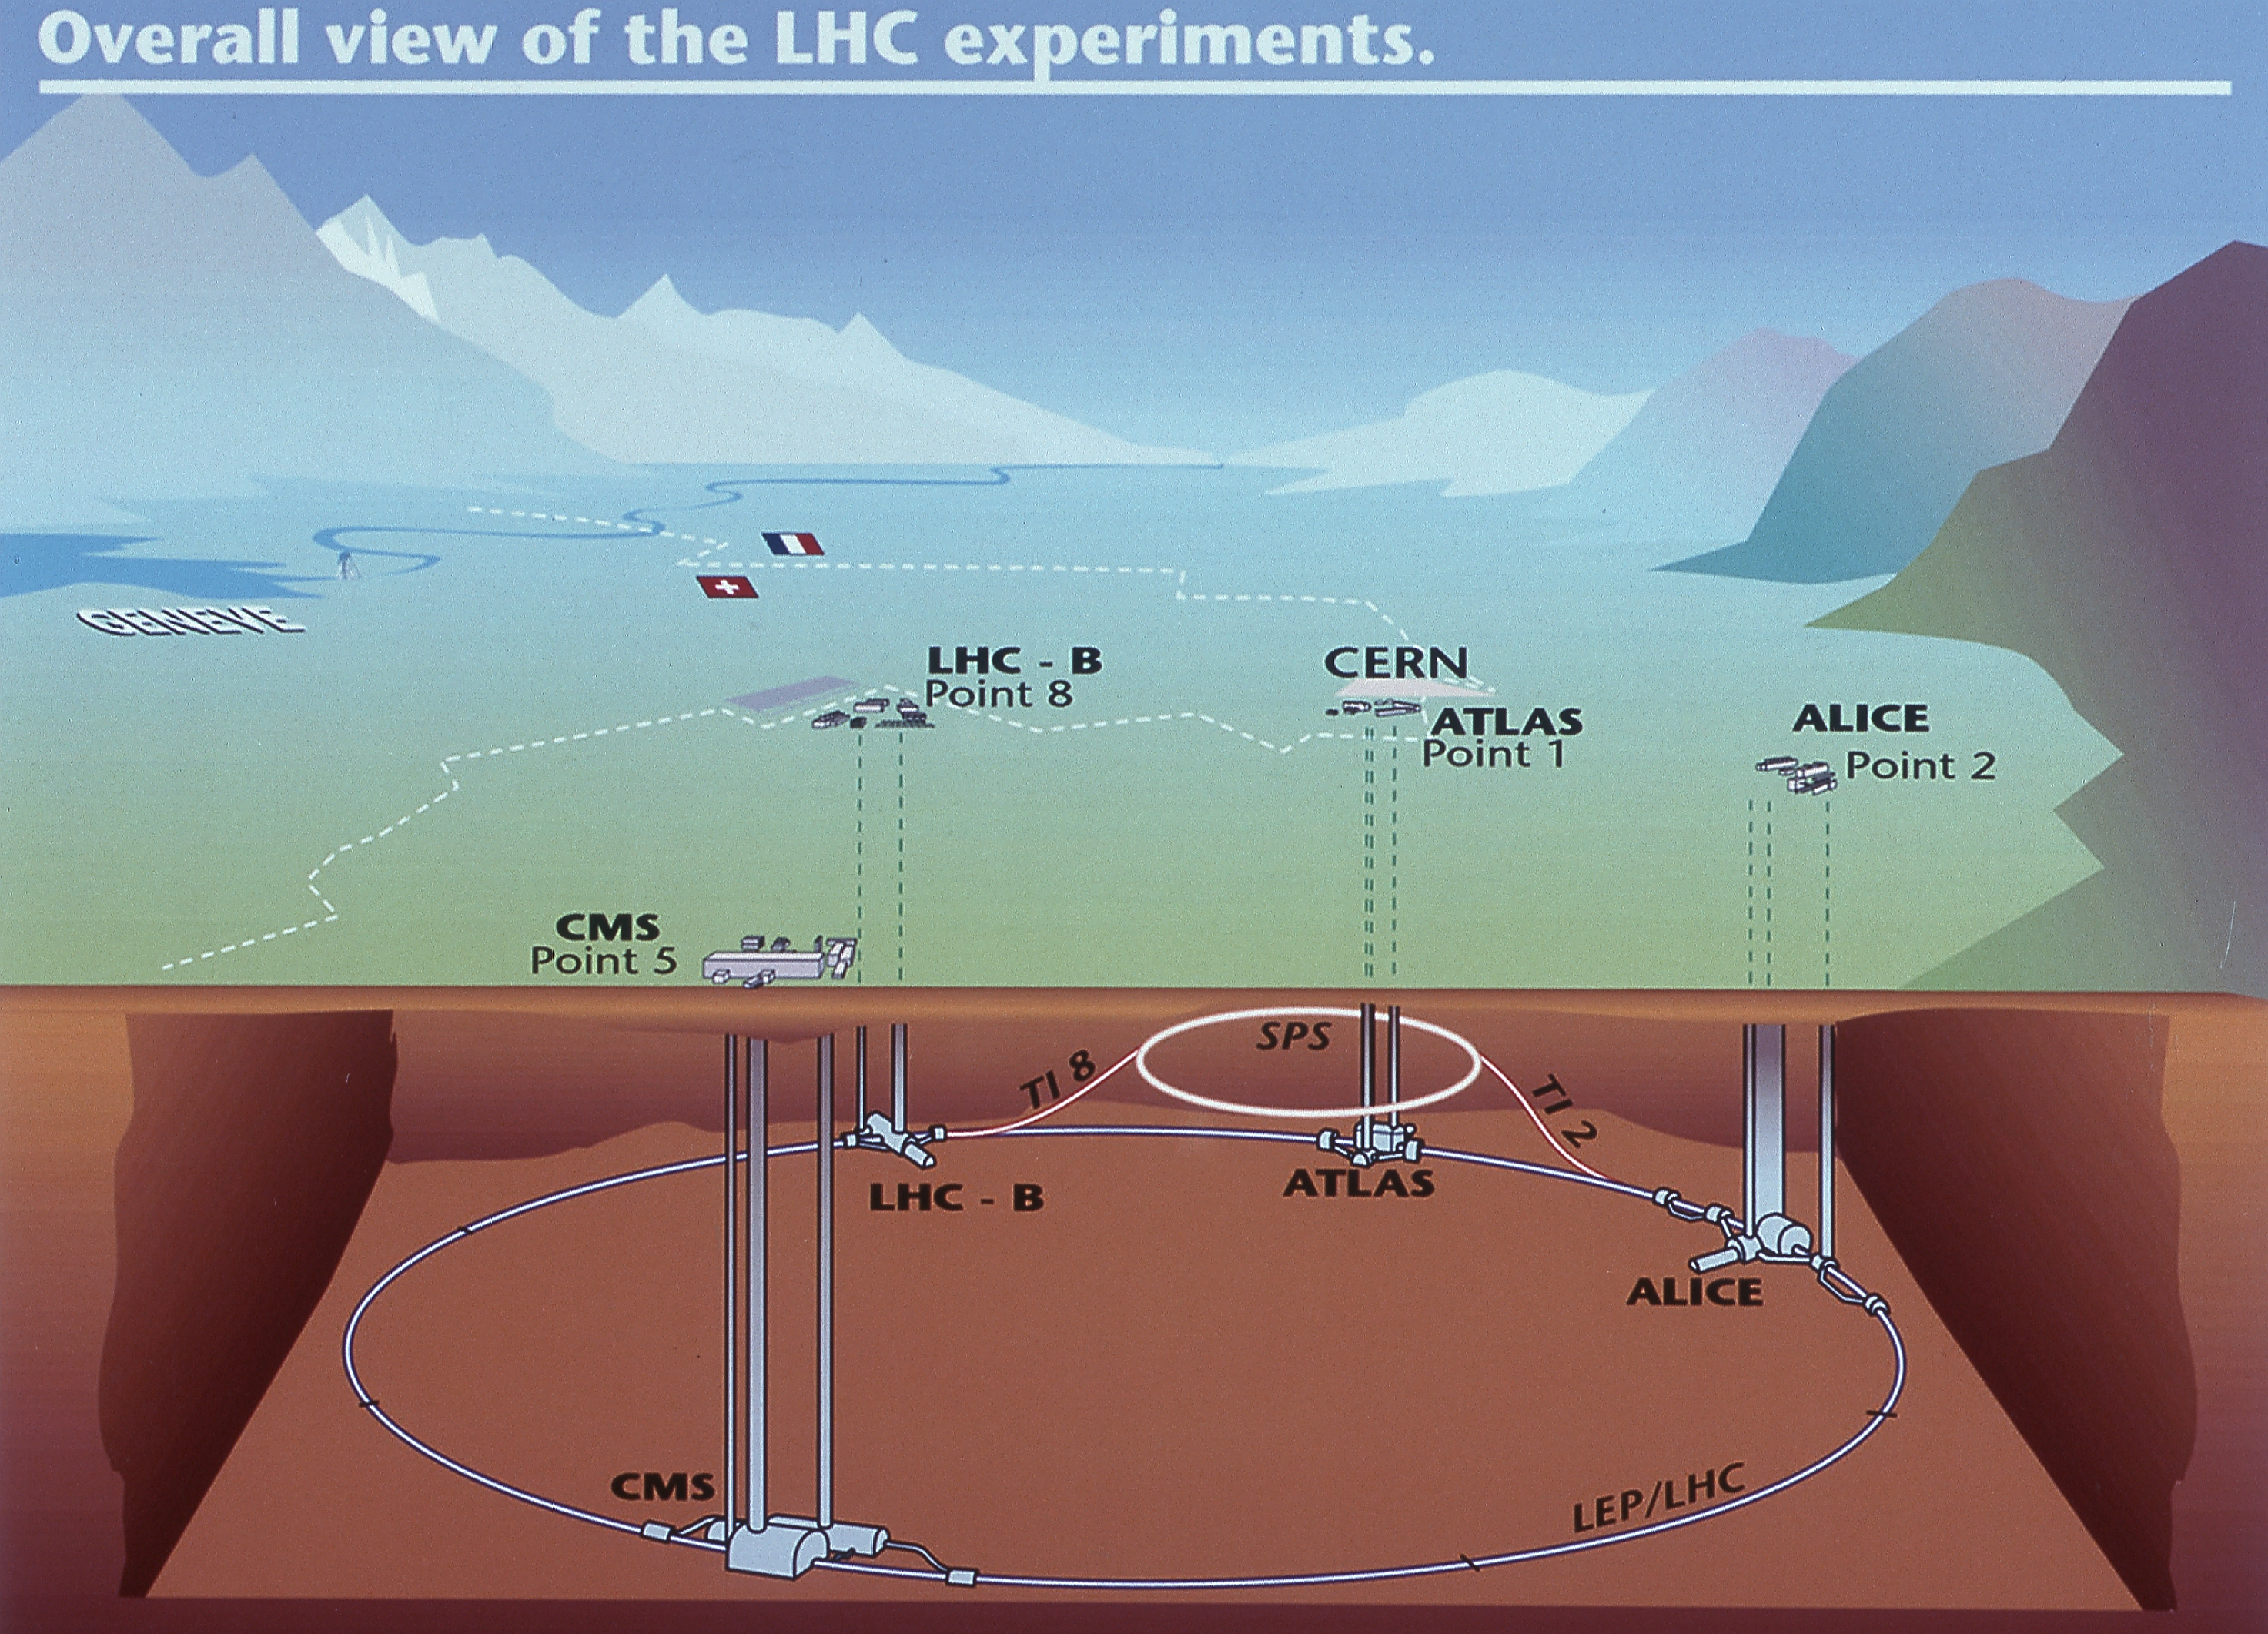
\includegraphics[width=0.9\textwidth]{figures/Detector/AtlasSite.jpg}
  \caption{The LHC and the sites of the 4 main LHC experiments.}
\label{Det:LHC}
\end{figure}

A series of accelerators provide proton bunches to the LHC at an energy of 450 GeV.
The proton bunches are then accelerated around the LHC by an array of superconducting dipole magnets to provide a beam energy up to 7 TeV.


\subsection{Luminosity}

The event rate of a process X is
\begin{equation}
R_X = L \sigma_X,
\label{Det:Lumi}
\end{equation}
where $\sigma_X$ is the cross section for the process and L is the luminosity.

Achieving a large luminosity is important for observing physics processes that have a low cross-section, and an accurate luminosity determination is important for measuring differential cross-sections of processes from the event rate. 

Luminosity is defined by,
\begin{equation}
L=\frac{N_b^2n_bf_{rev}\gamma_r}{4\pi\epsilon_n\beta^\star}F
\label{Det:Lumi}
\end{equation}
where $N_b$ is the number of particles per bunch, $n_b$ is the number of colliding bunches per beam, $f_{rev}$ is the revolution frequency, $\gamma_r$ is the relativistic gamma factor, $\epsilon_n$ is the normalised transverse beam emitance, $\beta^\star$ is the $\beta$ function at the interaction point, and $F$ is the geometric luminosity reduction factor due to the crossing angle of the beams.


Equation \ref{Det:Lumi} is useful to understand both the luminosity and how to increase it. 
However, the beam current changes throughout a run, so the equation is not ideal to measure the luminosity during a run.
*I am ot sure this is the only reason, it may also be due to the precision of the beam current measurement* 
An alternative way of acquiring the instantaneous luminosity is to measure the interaction rate via various ATLAS detectors and correlate this to the luminosity. 
The interaction rate is either the hit rate or the event rate for a given detector.
The luminosity defined by the interaction rate is,
\begin{equation}
L=\frac{\mu n_bf_{rev}}{\sigma_{inel}}=\frac{\mu_{vis}n_bf_{rev}}{\sigma_{vis}}
\label{Det:Lumi2}
\end{equation}
where $\mu$ is the number of inelastic collisions per bunch crossing, $\sigma_{inel}$ is the inelastic cross-section, $\mu_{vis}$ is the number of visible inelastic collisions per bunch crossing, and $\sigma_{vis}$ is visible inelastic cross-section. 


The calibration constant that associates the luminosity to the $\mu_{vis}$, which is measured using interaction rates, is $\sigma_{vis}$.
One method of obtaining the calibration constant $\sigma_{vis}$, and thus the absolute luminosity, is using a van der Meer scan method.
The method aims to measure the interaction rate when the two beams are perfectly aligned, while also measuring the beam currents.
This is achieved by scanning one beam over the other in the x-y plane. 
The interaction rate is fitted as a function of separation in x and y separately, and the maximum interaction rate is found at the peak of each fit. 
The 2010 data luminosity calibrated by the van der Meer scan method has a luminosity uncertainty of 3.4\%.

The amount of data that an experiment collects is expressed using the integrated luminosity, which is the integral over time of the luminosity.

\subsubsection{2010 run}
The 7 TeV centre-of-mass proton-proton run in 2010 was the first substantial data-taking period provided by the LHC. 
The initial runs provided peak luminosity of \lumi{\sim0.01\times10^{30}} from one pair of interacting bunches with a very low number of protons per bunch. 
By the end of the 2010 data-taking run the peak luminosity was \lumi{\sim2\times10^{32}} from 348 colliding bunches.
The luminosity increase was mainly achieved by increasing the number of colliding bunches per beam and the number of protons per bunch, though decreasing the $\beta^\star$ and reducing the beams crossing angle also increased the luminosity.


The 2010 data taking run was split into different data periods, where a new period would be started when there was a significant change in the beam parameters.
Table \ref{Det:Periods} shows the data periods for the 2010 LHC run, and how the beam conditions and peak luminosity changed.  
Additionally, periods G-I had used bunch trains where bunches were grouped together with 150 ns spacing between the bunches.  


The total integrated luminosity delivered by the LHC for the 2010 run was 48.1 $pb^1$.

\begin{table}
\begin{center}
\begin{tabular}{|c|c|c|c|c|}
\hline
Period&Date&Peak Luminosity& $N_b$ & $n_b$ \\
& &\lumi{}& $\times10^{11}$ & \\
\hline
A & Mar 30 - Apr 18 & 0.004 & <0.01 & 1 \\
B & Apr 23 - May 17 & 0.06 & 0.01-0.6 & 1-3 \\
C & May 18 - June 5 & 0.2 & 0.7-1.9 & 3-8 \\
D & June 18 - July 19 & 1.6 & 3-8 & 2-8 \\
E & July 29 - Aug 18 & 3.9 & 12-14 & 16 \\
F & Aug 19 - Aug 30 & 10 & 35-100 & 32-36 \\
G & Sept 22 - Oct 7 & 70 & 100-200 & 50-186 \\
H & Oct 8 - Oct 18 & 150 & 250-350 & 233-300 \\
I & Oct 24 - Oct 29 & 210 & 350-400 & 300-350 \\
\hline
\end{tabular}
\caption{ Beam information for the different data taking periods.}
\label{Det:Periods}
\end{center}
\end{table}


%\input{Detector/Coordinate.tex}
%\input{Detector/ATLAS.tex}
%\input{Detector/DetectorOverview.tex}  %{sec:Det:Over}
%\input{Detector/Magnet.tex}
%\input{Detector/InnerDetector.tex}
%\input{Detector/Calorimeter.tex}
%\subsection{Muon Detectors}

Furthest from the interaction point are the muon detectors. 
The muon detectors measure the hits from muons which are bent by the magnetic fields from the barrel toroid  and end-cap toroids, and a combination of both in the region between. 
The muon system has separate dedicated detectors for both precision position measurements and for triggering on muons.

For the precision measurement, Monitored Drift Tubes (MDT) are used in the rapidity range $|\eta|<2.7$, with the higher granularity Cathode Strip Chambers (CSC) used in the more forward region of $2<|\eta|<2.7$ in the innermost layer. 

The muon triggering system consists of Resistive Plate Chambers (RPC) in the barrel region and Thin Gap Chambers (TGC) in the end-cap region. 
The muon triggering system covers the region of $|\eta|<2.4$. 



%\subsection{Trigger and Data Acquisition}
\label{sec:Det:Trig}
The event rate from the LHC is $\sim1$ GHz, but only $\mathcal{O}(200~\rm Hz)$ will be recorded to disk. 
The ATLAS trigger and data acquisition system (TDAQ) reduces the initial event rate by select the most interesting events containing high \pt{} objects.
TDAQ is split into subsystems that are approximately associated with the sub-detectors previously described. 
The three different trigger levels are level 1 (L1), level 2 (L2), and event filter (EF). 
The L2 and EF triggers are called the higher level triggers (HLT). 
The trigger levels are applied in series, with each level refining the decision and adding additional requirements. 
L1 is required to make a decision in less than $2.5~\mu$s and reduce the rate to 75 kHz. 
If the event has passed a L1 trigger, it then goes through the L2 and EF trigger which have more information about the event and reduce the rate to 200Hz.
While the trigger is deciding if the event should be kept, the data acquisition system is buffering the event information.


L1 triggers try and select interesting objects, such as high $p_T$ jets, electrons, muons, photons, taus or large missing $E_T$, which are indicative of interesting physics processes. 
The main three detector systems that trigger events at the L1 level are the RPC and TGC, which trigger on muons, the calorimeter with reduced granularity, which triggers on the jets, electrons, muons, photons, or large missing $E_T$, and the Minimum Bias triggers that trigger on minimal energy and used to select an unbiased sample of events. 
The results from the muon, calorimeter and minimum bias triggers are passed to the Central Trigger Processors (CTP). 
The CTP then applies a trigger menu, which is list of triggers, their thresholds and prescales. 
By applying a prescale, $p$, to a trigger, only $\frac{1}{p}$ of the events that fired the trigger will be passed to L2. 
The purpose of the prescale is to reduce the rate of less interesting or high rate processes and also to keep the overall rate constant as the luminosity changes.

Should the event fire the L1 trigger and pass the prescale, the L1 trigger passes the region of interest, RoI, (this is a $\eta\phi$ region near the triggered object) to the HLT.
The L2 triggers have access to the information around the L1 RoI, but cannot attempt a  full event reconstruction in the 40 ns given to make the initial decision. 
The extra information at L2 is used to make tighter cuts in order to reduce the rate to 3.5 kHz.
The EF triggers have approximately four seconds to make a decision.
This is long enough to do longer offline analysis procedures using the full event reconstruction, which help to reduce the overall rate written to disk to 200 Hz.

The important triggers for this thesis are the calorimeter trigger (specifically the jet trigger) and the minimum bias trigger, which will be discussed below.
Additional information about the triggers and their performance can be found in \cite{ref:TriggerPerf}.

\subsubsection{Minimum Bias Triggers}
The minimum bias (Min Bias) triggers aim to provide events that are minimally biased towards any particular physics process. 
This is achieved by having a set of minimum bias trigger scintillator counters (MBTS) at the front of the calorimeter end-caps ($2<|\eta|<3.8$). 
The MBTS are fired by any low energy particle within their acceptance. 
The result is a very high rate from the MBTS, such that it is heavily prescaled for all but the lowest luminosity runs. 



\subsubsection{L1 Calorimeter}
The L1 calorimeter trigger (L1Calo) is the trigger system concerned with both the EM calorimeter and the hadronic calorimeter. 
The EM and hadronic calorimeter readout cells are merged into trigger towers of $\Delta\eta \times \Delta\phi$ of $0.1 \times 0.1$ for the precision region and increasing size for regions of higher rapidity. 
Trigger towers are used to define jet, electron, photon and tau trigger objects.

\subsubsection{Jet Triggers}

L1 jet trigger objects are found by first defining jet elements from 2x2 trigger towers in both the EM and hadronic calorimeters.
In the central precision region the jet elements cover a region of $\Delta\eta \times \Delta\phi = 0.2\times 0.2$. 
A sliding window algorithm is used to find the L1 jet objects. 
The algorithm can be set to have a window of either $2\times3$, $3\times3$ or $4\times4$ jet elements for the jet finding. 
The algorithm looks over the jet elements to find local maxima in transverse energy, \et{}, and defines a jet if the \et{} is  greater than a given threshold. 
The L1 jet triggers are named L1\_JX where X is the EM energy threshold for the jet object.

Once the L1 jets are found, the RoIs, corresponding to the position of the L1 jets, are passed to the HLT, and act as seeds. 
The L2 jet trigger can access the course calorimeter information from around the L1 jet RoI. 
This information is then passed into a seeded cone jet algorithm (see Section \ref{HLTCalo:Jets}), which is a basic and fast jet finder which uses jet radius, R, of 0.4, and which is restricted to three iterations.
The L2 can access finer calorimeter information and produce cone-like jets.
The hadronic components of the jet at L2 are calibrated, which is important as the detector has a lower response to hadronic energy deposits than the EM energy deposits. 

The EF jet triggers were not used in the 2010 data-taking. 
The definition in 2011 is in Section \ref{HLTCalo:Jets}.

%https://twiki.cern.ch/twiki/pub/Atlas/TapmJet/jetslice_v3_6April08.pdf


 
%\section{Jets in ATLAS}
\label{sec:Det:Jets}

The jet definition within ATLAS uses the \antikt{} algorithm, which is described in Section \ref{sec:Theory:Jets}. 
This algorithm groups related energy deposits in the ATLAS calorimeters.
Different input objects can be used with the \antikt{} algorithm, such as cells, towers and topoclusters and these objects can be calibrated to different energy scales.
In this analysis, unless otherwise stated, the jets are defined using the \antikt{} algorithm with a distance parameter of 0.6 running over topocluster at EM scale, where topoclusters and EM scale are defined in Section \ref{sec:Det:Calo}.


\subsubsection{Jet Energy Scale (JES)}

The jet response needs to be calibrated to take into account both detector and physics responses such as dead material, particle being bent into and  out of the jet, and noise threshold variation. 
Also, jets are found using EM-scale topoclusters and need to be calibrated due to the non-compensation of the hadronic calorimeter which has a lower detector response to hadrons than to EM deposits.
An EM+JES calibration was determined as a function of the jet \pt{} and rapidity to account for these effects.

The EM+JES calibration was done in three consecutive corrections.
The first was a pile-up offset correction designed to subtract energy contributions due to additional $pp$ interactions.
The correction is presented in \cite{ref:OffsetCorrection}, where the average energy in towers is considered as a function of $\eta{}$, the number of primary vertices and the bunch spacing.
The second correction was the vertex correction, which defined the origin of the jets to be the primary vertex.
This correction changes the direction and \pt{} of the jet, but not the energy, and it improves the angular resolution of the jet.
The original uncorrected $\eta{}$ is defined as the detector $\eta$.
The final correction is the jet energy scale (JES) correction.

The JES correction uses fully simulated MC, ``reco'', jets and jets at hadron level, ``truth'' jets, to obtain correction factors as a function of jet energy and jet rapidity. 
The response of the calorimeter to jets can be defined using these fully simulated MC samples as
\begin{equation}
\mathcal{R(\eta)} = \frac{\pt{}^{reco}(\eta)}{\pt{}^{truth}(\eta)}
\label{JetPerf:MCJetResp}
\end{equation}
where \pt{}$^{reco}$ is the \pt{} of the MC jet after full simulation of the detector, and  \pt{}$^{truth}$ is the \pt{} of the MC jet at hadron level.
The truth and reco jets are matched using a \dr{} requirement of 0.3.
The correction factors are calculated as a function of the jet's detector $\eta$ opposed to the vertex corrected $\eta$, as they represent calibrations for different detectors, and also as a function of the energy, as the detector responds to energy. 
Figure \ref{Det:MCResp} shows the jet responses, at EM scale, as a function of detector $|\eta|$ for different jet energies. 
From the comparison between fully simulated MC jets and truth jets, a small correction on the jet rapidity is calculated. 
This is due to part of jets falling into regions with lower response, giving a $\eta$ shift towards the higher responding areas. 
The original derivation of these factors can be found in \cite{ref:OffsetCorrection,ref:JES,ref:JES_basic}.

\begin{figure}
\centering
\mbox{
              %\epsfig{figure=figures/JetPerformance/MCResponse-ref_ATLAS-CONF-2010-055.eps,width=\textwidth}
              \epsfig{figure=figures/Detector/JetCalibfig_JES_vs_eta_Binning.eps,width=\textwidth}

                              }
\caption[Jet response for different regions of the ATLAS calorimeter]{ 
PYTHIA simulated jet EM-scale response as a function of reconstructed jet detector $\eta$ for different jet energies \cite{ref:JES}.
The different evaluated regions are shown, as well as their relation to the detector geometry. 
\label{Det:MCResp}
}
\end{figure}


\subsubsection{Jet Energy Scale Uncertainty}

The EM+JES method of calibration is based primarily on the ability of the MC to correctly simulate the ATLAS detector and also to model the physics effects such as energy flow out of the jet.
In-situ methods are used to validate the JES calibration and assign an uncertainty.
The JES uncertainty is derived from in-situ data measurements and also by varying MC settings. 
It is determined by combining the non-closure of the EM+JES on fully simulated MC jets, calorimeter response to isolated hadrons using test-beam information and in-situ methods, additional detector material, noise thresholds, differences compared to other MCs, uncertainties due to pile-up and \pt{} balance of dijet events. 


\begin{figure}
\centering
\mbox{
              \epsfig{figure=figures/Detector/JESSummary_JESUncertainty_AntiKt6Topo_EMJES2.1-2.8.eps,width=0.8\textwidth}

                              }
\caption[JES Uncertainty]{ 
Fractional JES uncertainty for jets with $2.1\le|\eta|\le2.8$ as a function of the jet \pt{} \cite{ref:JES}. 
\label{Det:JESU}
}
\end{figure}

Figure \ref{Det:JESU} shows the fractional JES uncertainty for jets with $2.1\le|\eta|\le2.8$ as a function of the jet \pt{}.
The dominant systematic at high \pt{} is the single particle response which comes from test-beam single pion information and the calorimeter response for a single hadron.
At low \pt{}, dijet balance (intercalibration) is the most significant uncertainty.
Dijet balance is an in-situ method of extending the uncertainty in the central region to other regions of the detector, and will be discussed in more detail in Chapter \ref{chp:JetPerf}.


\subsubsection{Jet Energy Resolution}

The jet energy resolution (JER) is a measure of the expected range of measured jet \pt{} compared to the original object. 
Some causes of the fluctuations in the measurement of a jet \pt{} are different hadron/EM contributions, non-average amount of additional energy from pile-up, and statistical fluctuations in the sampling technique across multiple calorimeter layers.
The JER was determined using the bi-sector method and the \pt{} balance of dijet events described in \cite{ref:JER,ref:JER2}. 




\subsubsection{Jet Cleaning}

Jets produced in an event need to be discriminated from ``bad'' background jets that come from  HEC spikes and EM noise in the calorimeter, cosmic rays or non-collision background.
Table \ref{det:Cleaning} shows the loose and medium cleaning requirements used to remove the bad jets where
\begin{itemize}
  \item The jet charge fraction, $\mathbf{f_{CH}}$, is the ratio of the sum of the \pt{} of tracks associated to the jet to the calibrated jet \pt{};
  \item  $\mathbf{f_{EM}}$ is the fraction of the jet EM scale energy that comes from EM clusters;
  \item  $\mathbf{f_{HEC}}$ is the fraction of the jet energy that was measured in the HEC;
  \item The LAr quality, $\mathbf{Q_{LAr}}$, is the fraction of the jet energy coming from LAr cells with poor signal shape quality;
  \item The HEC quality, $\mathbf{Q_{HEC}}$, is the fraction of the jet energy coming from HEC cells with poor signal shape quality;
  \item \Bold{neg. E} is the sum of the negative energy cells in the jet;
  \item Jet time, \Bold{t}, is the mean time between the cells in the jet and the event time;
  \item $\mathbf{f_{max}}$ is the maximum energy fraction in one calorimeter layer.
\end{itemize}

Jets coming from HEC spikes have most of the energy coming from a single noisy calorimeter cell, and so a $f_{HEC}$ requirement is applied to ensure energy deposits outside the HEC form a significant part of the total energy.
Fake jets coming from EM coherent noise are removed by cutting on the fraction of EM energy.
Finally, jets from non-collision backgrounds and cosmic rays are removed using a combination of timing and energy layer requirements.

The loose cleaning requirements are defined to have an efficiency of greater than 99\% for good jets, but a fraction of bad jets still remain. 
Whilst the medium cleaning requirements remove a higher proportion of bad jets, they have inefficiencies at low \pt{} for good jets. 

While the bad jets do not come from energy deposits from the interaction, there is a subset of jets, called ``ugly'' jets, which are energy deposits from the interaction which have been badly measured. 
Ugly jets are often found in regions between detectors, ``cracks'' regions, where the performance of the detectors are not optimal.
Two selection criteria are applied to remove ugly jets.
First, the jet energy which falls into the transition between the barrel and the end-cap is required to be less that half the total jet energy.
Second, the fraction of energy that comes from bad cells inside the jet is required to be less than half of the total jet energy.


\begin{table}
\begin{center}
\footnotesize

\begin{tabular}{|c||c|c|}
\hline
& Loose & Medium = Loose OR \\
\hline
            & $\rm f_{HEC}<0.5$ \& $|\rm Q_{HEC}|>0.5$                         &                                                              \\
HEC spikes  &              or                                              & $\rm f_{HEC}>1-|Q_{HEC}|$                                          \\
            &  $\rm |neg.E|>60$ GeV                                        &                                                              \\
\hline
EM          &                                                              &                                                              \\
coherent    & $\rm f_{EM} >0.95$ \& $\rm |Q_{LAr}| >0.8$ \& $|\eta|<2.8$     &   $\rm f_{EM} >0.9$ \& $\rm |Q_{LAr}| >0.8$ \& $|\eta|<2.8$    \\
noise       &                                                              &                                                              \\
\hline
            &           $\rm |t|>25$ ns                                                    &                                                              \\
Non-        &              or                                              &  $\rm |t|>10$ ns                                          \\
collision   & $\rm f_{EM} <0.05$ \& $\rm f_{CH}<0.05$ \& $|\eta|<2$     &   or     \\
background  &        or                     &   $\rm f_{EM}<0.05$ \& $\rm f_{CH} <0.1$ \& $|\eta|<2$    \\
\& cosmics  & $\rm f_{EM} <0.05$ \&  $|\eta|>2$     &   or     \\
            &        or                     &   $\rm f_{EM}>0.95$ \& $\rm f_{CH} <0.05$ \& $|\eta|<2$    \\
             & $\rm f_{max}<0.99$ \&  $|\eta|<2$     &        \\

\hline

\end{tabular}
\caption[Jet Cleaning Definitions]{
Loose and Medium jet cleaning definitions.
\label{det:Cleaning}
}
\end{center}
\end{table}


 
%
%\chapter{High Level Trigger Calorimeter Monitoring}
%\label{chp:HLTCalo}
%The calorimeter high-level trigger (HLTCalo) is used to trigger on physics objects that deposit their energy in either the electromagnetic or hadronic calorimeter.
As described in Section \ref{sec:Det:Calo}, the calorimeter is segmented into cells.
These cells are clustered together and can be combined with inner detector tracks to define physics objects such as electrons, photons, taus, and jets. 

The HLTCalo is monitored to check the performance and consistency of the triggers. 
This is achieved by monitoring the individual cells in the calorimeters and also by comparing the different L2 and EF triggered physics objects to the corresponding offline object.
Flags are defined for each monitoring distribution, where a green flag represents the distribution is consistent with the expected distribution, and yellow and red represent a deviation from the expected distribution. 
When the flag is red or yellow the distribution is studied further via a web based graphical user interface to find the reason, and if necessary the associated data can then be excluded from physics analysis.


In this chapter, work done by the author on improvements to the current cell monitoring which expose hot cells, and the addition of monitoring of calorimeter objects are discussed. 

\section{Cells}

The overall HLTCalo monitoring is done on a cell by cell basis.
This monitoring consists of distributions showing the number of active cells in the LAr and Tile calorimeters, the number of problematic cells and the position of these cells in the LAr and Tile calorimeters, and also the difference in cell energy between the trigger levels and offline levels.

The number of cells in the LAr and Tile calorimeters is an example of a monitoring plot that is very stable and should only change when a hot cell is masked or taken offline, allowing very tight flag definitions.
Monitoring plots, such as the percentage difference in energy in the trigger and offline cells, vary significantly ($\approx15\%$) with different running conditions, so either looser or no flag definitions are set.

The average transverse energy per cell in $\eta  \phi$ distribution is important in identifying hot spots where one cell records artificially high energy in every event.
Hot cells can be caused from electronic problems within the cells. 
Figure \ref{SW_hotspot} shows an example of a hot spot found using the offline cell monitoring in run 201191. 
This resulted in the cell being masked.

\begin{figure}
\centering
\mbox{
   \includegraphics[width=0.9\textwidth]{figures/ServiceWork/Cells_HotSpot-Edit.pdf}
}
\caption[Average \et{} for HLT calorimeter cells]{
Average \et{} per $\eta \phi$ bin in run 201191. 
A hot region is observed at $\eta=2.5$ $\phi=1$. 
\label{SW_hotspot}}
\end{figure}



\section{Calorimeter Objects}

The HLTCalo is also monitored by comparing calorimeter triggered objects (electrons, photons and jets) to the offline objects.
A cut on the \dr{} is made to match the triggered objects to the offline objects.
An \et{} cut has been applied to the offline objects, which is the same as required by the analysis selection. 



\subsection{Electrons and Photons}



\input{ServiceWork/Egamma.tex}
 
\subsection{Jets}
\label{HLTCalo:Jets}

\section{Jets in ATLAS}
\label{sec:Det:Jets}

The jet definition within ATLAS uses the \antikt{} algorithm, which is described in Section \ref{sec:Theory:Jets}. 
This algorithm groups related energy deposits in the ATLAS calorimeters.
Different input objects can be used with the \antikt{} algorithm, such as cells, towers and topoclusters and these objects can be calibrated to different energy scales.
In this analysis, unless otherwise stated, the jets are defined using the \antikt{} algorithm with a distance parameter of 0.6 running over topocluster at EM scale, where topoclusters and EM scale are defined in Section \ref{sec:Det:Calo}.


\subsubsection{Jet Energy Scale (JES)}

The jet response needs to be calibrated to take into account both detector and physics responses such as dead material, particle being bent into and  out of the jet, and noise threshold variation. 
Also, jets are found using EM-scale topoclusters and need to be calibrated due to the non-compensation of the hadronic calorimeter which has a lower detector response to hadrons than to EM deposits.
An EM+JES calibration was determined as a function of the jet \pt{} and rapidity to account for these effects.

The EM+JES calibration was done in three consecutive corrections.
The first was a pile-up offset correction designed to subtract energy contributions due to additional $pp$ interactions.
The correction is presented in \cite{ref:OffsetCorrection}, where the average energy in towers is considered as a function of $\eta{}$, the number of primary vertices and the bunch spacing.
The second correction was the vertex correction, which defined the origin of the jets to be the primary vertex.
This correction changes the direction and \pt{} of the jet, but not the energy, and it improves the angular resolution of the jet.
The original uncorrected $\eta{}$ is defined as the detector $\eta$.
The final correction is the jet energy scale (JES) correction.

The JES correction uses fully simulated MC, ``reco'', jets and jets at hadron level, ``truth'' jets, to obtain correction factors as a function of jet energy and jet rapidity. 
The response of the calorimeter to jets can be defined using these fully simulated MC samples as
\begin{equation}
\mathcal{R(\eta)} = \frac{\pt{}^{reco}(\eta)}{\pt{}^{truth}(\eta)}
\label{JetPerf:MCJetResp}
\end{equation}
where \pt{}$^{reco}$ is the \pt{} of the MC jet after full simulation of the detector, and  \pt{}$^{truth}$ is the \pt{} of the MC jet at hadron level.
The truth and reco jets are matched using a \dr{} requirement of 0.3.
The correction factors are calculated as a function of the jet's detector $\eta$ opposed to the vertex corrected $\eta$, as they represent calibrations for different detectors, and also as a function of the energy, as the detector responds to energy. 
Figure \ref{Det:MCResp} shows the jet responses, at EM scale, as a function of detector $|\eta|$ for different jet energies. 
From the comparison between fully simulated MC jets and truth jets, a small correction on the jet rapidity is calculated. 
This is due to part of jets falling into regions with lower response, giving a $\eta$ shift towards the higher responding areas. 
The original derivation of these factors can be found in \cite{ref:OffsetCorrection,ref:JES,ref:JES_basic}.

\begin{figure}
\centering
\mbox{
              %\epsfig{figure=figures/JetPerformance/MCResponse-ref_ATLAS-CONF-2010-055.eps,width=\textwidth}
              \epsfig{figure=figures/Detector/JetCalibfig_JES_vs_eta_Binning.eps,width=\textwidth}

                              }
\caption[Jet response for different regions of the ATLAS calorimeter]{ 
PYTHIA simulated jet EM-scale response as a function of reconstructed jet detector $\eta$ for different jet energies \cite{ref:JES}.
The different evaluated regions are shown, as well as their relation to the detector geometry. 
\label{Det:MCResp}
}
\end{figure}


\subsubsection{Jet Energy Scale Uncertainty}

The EM+JES method of calibration is based primarily on the ability of the MC to correctly simulate the ATLAS detector and also to model the physics effects such as energy flow out of the jet.
In-situ methods are used to validate the JES calibration and assign an uncertainty.
The JES uncertainty is derived from in-situ data measurements and also by varying MC settings. 
It is determined by combining the non-closure of the EM+JES on fully simulated MC jets, calorimeter response to isolated hadrons using test-beam information and in-situ methods, additional detector material, noise thresholds, differences compared to other MCs, uncertainties due to pile-up and \pt{} balance of dijet events. 


\begin{figure}
\centering
\mbox{
              \epsfig{figure=figures/Detector/JESSummary_JESUncertainty_AntiKt6Topo_EMJES2.1-2.8.eps,width=0.8\textwidth}

                              }
\caption[JES Uncertainty]{ 
Fractional JES uncertainty for jets with $2.1\le|\eta|\le2.8$ as a function of the jet \pt{} \cite{ref:JES}. 
\label{Det:JESU}
}
\end{figure}

Figure \ref{Det:JESU} shows the fractional JES uncertainty for jets with $2.1\le|\eta|\le2.8$ as a function of the jet \pt{}.
The dominant systematic at high \pt{} is the single particle response which comes from test-beam single pion information and the calorimeter response for a single hadron.
At low \pt{}, dijet balance (intercalibration) is the most significant uncertainty.
Dijet balance is an in-situ method of extending the uncertainty in the central region to other regions of the detector, and will be discussed in more detail in Chapter \ref{chp:JetPerf}.


\subsubsection{Jet Energy Resolution}

The jet energy resolution (JER) is a measure of the expected range of measured jet \pt{} compared to the original object. 
Some causes of the fluctuations in the measurement of a jet \pt{} are different hadron/EM contributions, non-average amount of additional energy from pile-up, and statistical fluctuations in the sampling technique across multiple calorimeter layers.
The JER was determined using the bi-sector method and the \pt{} balance of dijet events described in \cite{ref:JER,ref:JER2}. 




\subsubsection{Jet Cleaning}

Jets produced in an event need to be discriminated from ``bad'' background jets that come from  HEC spikes and EM noise in the calorimeter, cosmic rays or non-collision background.
Table \ref{det:Cleaning} shows the loose and medium cleaning requirements used to remove the bad jets where
\begin{itemize}
  \item The jet charge fraction, $\mathbf{f_{CH}}$, is the ratio of the sum of the \pt{} of tracks associated to the jet to the calibrated jet \pt{};
  \item  $\mathbf{f_{EM}}$ is the fraction of the jet EM scale energy that comes from EM clusters;
  \item  $\mathbf{f_{HEC}}$ is the fraction of the jet energy that was measured in the HEC;
  \item The LAr quality, $\mathbf{Q_{LAr}}$, is the fraction of the jet energy coming from LAr cells with poor signal shape quality;
  \item The HEC quality, $\mathbf{Q_{HEC}}$, is the fraction of the jet energy coming from HEC cells with poor signal shape quality;
  \item \Bold{neg. E} is the sum of the negative energy cells in the jet;
  \item Jet time, \Bold{t}, is the mean time between the cells in the jet and the event time;
  \item $\mathbf{f_{max}}$ is the maximum energy fraction in one calorimeter layer.
\end{itemize}

Jets coming from HEC spikes have most of the energy coming from a single noisy calorimeter cell, and so a $f_{HEC}$ requirement is applied to ensure energy deposits outside the HEC form a significant part of the total energy.
Fake jets coming from EM coherent noise are removed by cutting on the fraction of EM energy.
Finally, jets from non-collision backgrounds and cosmic rays are removed using a combination of timing and energy layer requirements.

The loose cleaning requirements are defined to have an efficiency of greater than 99\% for good jets, but a fraction of bad jets still remain. 
Whilst the medium cleaning requirements remove a higher proportion of bad jets, they have inefficiencies at low \pt{} for good jets. 

While the bad jets do not come from energy deposits from the interaction, there is a subset of jets, called ``ugly'' jets, which are energy deposits from the interaction which have been badly measured. 
Ugly jets are often found in regions between detectors, ``cracks'' regions, where the performance of the detectors are not optimal.
Two selection criteria are applied to remove ugly jets.
First, the jet energy which falls into the transition between the barrel and the end-cap is required to be less that half the total jet energy.
Second, the fraction of energy that comes from bad cells inside the jet is required to be less than half of the total jet energy.


\begin{table}
\begin{center}
\footnotesize

\begin{tabular}{|c||c|c|}
\hline
& Loose & Medium = Loose OR \\
\hline
            & $\rm f_{HEC}<0.5$ \& $|\rm Q_{HEC}|>0.5$                         &                                                              \\
HEC spikes  &              or                                              & $\rm f_{HEC}>1-|Q_{HEC}|$                                          \\
            &  $\rm |neg.E|>60$ GeV                                        &                                                              \\
\hline
EM          &                                                              &                                                              \\
coherent    & $\rm f_{EM} >0.95$ \& $\rm |Q_{LAr}| >0.8$ \& $|\eta|<2.8$     &   $\rm f_{EM} >0.9$ \& $\rm |Q_{LAr}| >0.8$ \& $|\eta|<2.8$    \\
noise       &                                                              &                                                              \\
\hline
            &           $\rm |t|>25$ ns                                                    &                                                              \\
Non-        &              or                                              &  $\rm |t|>10$ ns                                          \\
collision   & $\rm f_{EM} <0.05$ \& $\rm f_{CH}<0.05$ \& $|\eta|<2$     &   or     \\
background  &        or                     &   $\rm f_{EM}<0.05$ \& $\rm f_{CH} <0.1$ \& $|\eta|<2$    \\
\& cosmics  & $\rm f_{EM} <0.05$ \&  $|\eta|>2$     &   or     \\
            &        or                     &   $\rm f_{EM}>0.95$ \& $\rm f_{CH} <0.05$ \& $|\eta|<2$    \\
             & $\rm f_{max}<0.99$ \&  $|\eta|<2$     &        \\

\hline

\end{tabular}
\caption[Jet Cleaning Definitions]{
Loose and Medium jet cleaning definitions.
\label{det:Cleaning}
}
\end{center}
\end{table}





\subsection{Summary}

Updates to the HLT cell monitoring and the addition of offline monitoring of the HLTCalo using physics objects such as jets are presented.
Cells have been masked to reduce the effect from noisy cells, and the EM and jet triggers have been monitored and observed to have good stability. 
Data where this has not been the case have not been used for physics analyses.

%
%\chapter{In-Situ Validation of ATLAS Jet Reconstruction and Calibration}
%\label{chp:JetPerf}
%The response of the calorimter to jets can be defined using fully simulated MC samples as
\begin{equation}
\mathcal{R(\eta)} = \frac{\pt{}^{reco}(\eta)}{\pt{}^{truth}(\eta)}
\label{JetPerf:MCJetResp}
\end{equation}
where \pt{}$^{reco}$ is the \pt{} of the MC jet after full simulation of the detector, and  \pt{}$^{truth}$ is the \pt{} of the MC jet, before detector simulation. 
The truth and reco jets are matched using a \dr{} cut of 0.3.
%The calibration is done using the H1 method, which is described in \cite{ref:H1}. 

Jet response within the calorimeter varies as a function of $\eta$ due to the different calorimeter technology used and the varying levels of dead material, as shown in Figure \ref{JetPerf:MCResp}.
The default calibration procedure in ATLAS is to correct the energy and momentum by $\frac{1}{\mathcal{R(\eta)}}$.

\begin{figure}
\centering
\mbox{
              {\epsfig{figure=figures/JetPerformance/MCResponse-ref_ATLAS-CONF-2010-055.eps,width=\textwidth}}
                              }
\caption[]{ PYTHIA simulated jet EM-scale response as a function of reconstructed jet $\eta$ for different jet energies \cite{ref:EtaInter2010}
\label{JetPerf:MCResp}}
\end{figure}

The accuracy of the calibration depends how well the MC models the physics, such as ..., and how accurately if describes the detector geometry. 
In-situ methods are used to check the calibration and to assign a corresponding uncertainty.


********Add a section on the JES uncertainty contributions and link to paper ******
In the central region (\etaRange{0}{0.8}), the response and uncertainty from single particles in the calorimeter is used to give the JES uncertainty.  
This is done by  studying the charged particle response of the detector, gained from comparing charged tracks to isolated energy deposits.
********


Outside of this central region different in-situ methods are used to get contributions to the JES uncertainty.
One of the in-situ methods used to assess the uncertainty in the end cap (\etaRange{0.8}{2.8}) and forward (\etaRange{2.8}{4.5}) regions is pseudorapidity inter-calibration using dijets.
The jets in the central region, which are well understood, are used as a baseline to get relative calibration uncertainties in the end cap and forward regions. 

This method of extending the uncertainty outside the central region is achieved by using the \pt{} balance of dijet events to get a relative jet response between the 2 jets.
In a dijet topology, it is expected, that both jets should have the same transvere momentum, assuming that the jets arise from a $2\rightarrow2$ partonic scatter.
Using this assumption, the \pt{} imbalance can be expressed using the asymmetry, $\mathcal{A}$, defined as
\begin{equation}
\mathcal{A} =\frac{\pt{}^1 - \pt{}^2}{\ptave{}},
\label{JetPerf:Assym}
\end{equation}
where $\pt{}^1$ and $\pt{}^2$ are the transverse momentum of the two leading jets, and $\ptave{}$ is the average \pt{} of the two jets.
For imperfectly measured jets, the asymmetry would not be unity and a relative calorimeter response to a jet can be constructed using the asymmetry as,
\begin{equation}
 \frac{\pt{}^1}{\pt{}^2}=\frac{2+\mean{\mathcal{A}}}{2-\mean{\mathcal{A}}}.
\label{JetPerf:JetResp}
\end{equation}


For the balancing to work it is important that there is no other hard QCD emission in the interaction, this is achieved with a cut on the 3rd jet $\pt{}^3<0.25*\ptave{}$ and requiring the jets to be back-to-back in azimuth with a cut $\dphi{}>2.6$.

 

%\section{In-Situ Validation of Jet Calibration}
%\input{JetPerformance/JESU_Standard.tex}
%\subsubsection{Matrix Method for Dijet Balance}

The matrix method differs from the standard method by not requiring a specific reference region.
Instead of a probe and reference jet, there is a ``left'' jet and a ``right'' jet, where $\eta_{\rm left}<\eta_{\rm right}$.
As a result Equations \ref{JetPerf:Assym} and \ref{JetPerf:JetResp} become,
\begin{equation}
\mathcal{A} =\frac{\pt{}^{left} - \pt{}^{right}}{\ptave{}}
\label{JetPerf:MM_Assym}
\end{equation}
and 
\begin{equation}
\frac{\pt{}^{left}}{\pt{}^{right}}=\frac{2+\mathcal{A}}{2-\mathcal{A}}
\label{JetPerf:MM_CorrectionFactor}
\end{equation}

For given values of $\eta^{left}$ and $\eta^{right}$, the relative response between the two regions can be defined as 

\begin{equation}
\mathcal{R_{\rm ijk}}= \frac{2-\mean{\mathcal{A_{\rm ijk}}}}{2+\mean{\mathcal{A_{\rm ijk}}}} = \frac{ c_{ik}^{left}}{ c_{jk}^{right}}
\label{JetPerf:MM_Response_Measured}
\end{equation}
where i, j and k are label bins in  $\eta^{left}$, $\eta^{right}$ and $\ptave{}$ respectively, and $\mean{\mathcal{A}}$ is the mean \footnote{The asymmetry distribution is fitted with a Gaussian function between -0.7 and 0.7, and the value of the fit is taken as the mean, unless there are low statistics, then the average of the asymmetry is taken} of the asymmetry distribution. 


For every k-th $\ptave{}$ bin, there exists $\sum\limits^N_{n=1}n$ relative responses, $\mathcal{R_{\rm ijk}}$, corresponding to different $\eta^{left}$ and $\eta^{right}$ bins (i,j).
A minimisation is performed to take into account the response measurements between many regions, to extract the inter-calibration factors for a specific $\eta$ region.
The inverse of the variance on each measured relative response, $\Delta\mathcal{R_{\rm ijk}}$, is used to weight the equations in a minimisation equation,
\begin{equation}
\sum\limits^N_{j=1} \sum\limits^N_{i=j}\left\{\frac{1}{\Delta\mathcal{R_{\rm ijk}}}( c_{jk}\mathcal{R_{\rm ijk}}- c_{ik} )\right\}^2 + X(c_{ik}).
\label{JetPerf:MM_Final}
\end{equation}

The first term in Equation \ref{JetPerf:MM_Final} is minimised to find the values of $c_{ik}$ that best agree with the measured $\mathcal{R_{\rm ijk}}$. 
A trivial undesired solution is $c_i=0$. 
The second term in \ref{JetPerf:MM_Final} is added to prevent this solution.
The specific form is 
\begin{equation}
X(c_{ik})= K(N^{-1}_{bins} \sum\limits^{N_{bins}}_{i=1} c_{ik} - 1 )^2,
\end{equation}
where K is a constant.
This term is a minimum when the average correction factor is equal to unity.
The constant, K, is set to $10^6$, and its purpose is to penalise deviations of the average away from 1. 
For large values of K, the correction factors found are stable.
Once the minimised $c_{ik}$ values are found, these values are rescaled such that the correction factors at $|\eta|<1$ are equal to unity. 

The advantage of this method with respect to the standard method is that each relative response is calculated using every $\eta$ bin combination, which gives an increase in the statistics used, especially at larger $\eta$, when compared to the standard method which needed one of the jets to be in the central probe region.

%\input{JetPerformance/JESU_Example.tex}
%\section{2011 Study of Pile-up Dependance}
%\subsubsection{Event Selection}

The jets in the analysis were reconstructed using the \antikt{} algorithm and calibrated using the JES scheme (discussed in Section \ref{sec:Det:Jets}).

The analysis requires that a single jet trigger has passed.
Triggers are used if they are in the plateau region of the turn-on curve, corresponding to a greater than $99\%$ efficiency.
The trigger used for a given \ptave{} is shown in Table \ref{JetPerf:Triggers}.
A trigger with name jX requires an EF-level trigger jet with EM scale $\pt{}>$X GeV.
\begin{table}
%\footnotesize
\centering
\begin{tabular}{  c c }
\ptave{} & Trigger\\
$[\rm GeV]$ & \\
\hline
$22-30$   & j10 \\
$30-40$   & j15 \\
$40-55$   & j20 \\
$55-75$   & j30 \\
$75-100$  & j40 \\
$100-130$ & j55 \\
$130-170$ & j75 \\
$170-220$ & j100 \\
$220-300$ & j135 \\
$300-400$ & j180 \\
\end{tabular}
\caption[]{
\label{JetPerf:Triggers}}
\end{table}
The data were required to be in luminosity blocks when all ATLAS sub-detectors are fully functioning. 

To ensure the two-to-two topology the \dphi{} between the two jets was required to be greater than $2.5$ rad and events containing a third jet with $\pt{} >0.25~ \ptave{}$ were removed.
The reference region that is used to do the final rescaling of the responses in the matrix method is \etarange{-0.8}{0.8}.

\subsubsection{Basic Asymmetry and Response Distributions}

Figures \ref{JetPerf:Asym_j15} and \ref{JetPerf:Asym_j30} each show two typical asymmetry distributions for jets falling in (a) two central regions, $-0.8<\eta_{left}<-0.1$ and $0.1<\eta_{right}<0.8$, and (b) one central region and one more forward region, $0.1<\eta_{left}<0.8$ and $2.1<\eta_{right}<2.8$. 
Each asymmetry distributions have been fitted with a Gaussian function from $\rm{-0.7<A<0.7}$.

Figure \ref{JetPerf:Asym_j15} shows typical asymmetry distributions, for $30<\ptave{}<40$ GeV jets.
The peak of the fitted asymmetry for both jets falling in the central region is $0.006$, which corresponds to a very small \pt{} imbalance of $\mean{\pt{}^{right}}= 0.994 \mean{\pt{}^{left}}$.
The peak of the fitted asymmetry for one jet falling in the central region and the other in a forward region is $0.023$, which corresponds to a \pt{} imbalance of $\mean{\pt{}^{right}}= 0.98 \mean{\pt{}^{left}}$.

Figure \ref{JetPerf:Asym_j30} shows typical asymmetry distributions, for $55<\ptave{}<75$ GeV jets.
The peak of the fitted asymmetry for both jets falling in the central region is $0.003$, which corresponds to very small \pt{} imbalance of $\mean{\pt{}^{right}}= 0.997 \mean{\pt{}^{left}}$. 
The peak of the fitted asymmetry for one jet falling in the central region and the other in a forward region is $0.007$, which corresponds to a \pt{} imbalance of $\mean{\pt{}^{right}}= 0.993 \mean{\pt{}^{left}}$.

The width in the asymmetry distributions arises due to the jet energy resolution of the two jets and the peak value of the fitted asymmetry relates to the relative responses of the two regions.
In the distributions for both the low and high \ptave{} jets, the case where both jets fall into central regions has a lower \pt{} imbalance than the case where one jet falls into a forward region.  
Both central jets fall into the regions of the barrel calorimeter when is well understood, and has little dead material.
However, when one jet is further forward, is falls into the end-cap region on the calorimeter and the difference observed could be due to the differing abilities to calibrate the different parts of the detector. 
Additionally, the higher \ptave{} jets have a smaller \pt{} imbalance than the lower \ptave{} jets.
The spread of asymmetry is smaller for higher \ptave{} jets, which is due to the improved resolution for higher \pt{} jets.


Figures \ref{JetPerf:ResponseMatrix_30_40_j15} and \ref{JetPerf:ResponseMatrix_55_75_j30} show the the response matrices, which are used by the minimisation, for jets in the range $30<\ptave{}<40$ GeV and $55<\ptave{}<75$ GeV respectively.
Generally, the low \ptave{} jets have a larger range of relative responses than the high \ptave{} jets, with some bins deviating from unity by up to $6\%$.
In both response matrices the higher $\eta$ bins have a larger spread of responses than the more central bins.


Figure \ref{JetPerf:PtComp} shows the relative response as a function of detector $\eta$ for $22<\ptave{}<30$ GeV jets, $30<\ptave{}<40$ GeV jets, and $55<\ptave{}<75$ GeV jets. 
The largest relative response occurs for low \ptave{}.
There is a relative response of $\approx1.02$ at $|\eta|=1$ which corresponds to the crack region between the tile barrel and tile extended barrel. 
This crack can be seen in the jet energy EM-scale response in Figure \ref{JetPerf:MCResp}.
For low \pt{} jets, the calibration has over-calibrated the jets in this crack region. 
For the medium and high jet \pt{} ranges shown, the relative response for $|\eta|<1$ is very close to unity.
The response at higher $\eta{}$ deviates away from unity, and as the jet \pt{} increases the deviation reduces. 
\begin{figure}
\centering
\mbox{
              \subfigure[]{\epsfig{figure=figures/JetPerformance/2011/j15zvar4_6.eps,width=0.5\textwidth}}
              \subfigure[]{\epsfig{figure=figures/JetPerformance/2011/j15zvar6_9.eps,width=0.5\textwidth}}
}
\caption[]{
Asymmetry distribution for jets with $30<\ptave{}<40$ GeV with (a) $-0.8<\eta_{left}<-0.1$ and $0.1<\eta_{right}<0.8$ and (b)  $0.1<\eta_{left}<0.8$ and $2.1<\eta_{right}<2.8$.
The distribution is fitted using a Gaussian function between $\rm{-0.7<A<0.7}$ and the fit result and error is shown as is the mean and error on the mean. 
\label{JetPerf:Asym_j15}}
\end{figure}

\begin{figure}
\centering
\mbox{
              \subfigure[]{\epsfig{figure=figures/JetPerformance/2011/j30zvar4_6.eps,width=0.5\textwidth}}
              \subfigure[]{\epsfig{figure=figures/JetPerformance/2011/j30zvar6_9.eps,width=0.5\textwidth}}
}
\caption[]{
Asymmetry distribution for jets with $55<\ptave{}<75$ GeV with (a) $-0.8<\eta_{left}<-0.1$ and $0.1<\eta_{right}<0.8$ and (b)  $0.1<\eta_{left}<0.8$ and $2.1<\eta_{right}<2.8$.
The distribution is fitted using a Gaussian function between $\rm{-0.7<A<0.7}$ and the fit result and error is shown as is the mean and error on the mean. 
\label{JetPerf:Asym_j30}}
\end{figure}

\begin{figure}
\centering
\mbox{
              \epsfig{figure=figures/JetPerformance/2011/j15TwoDPlotBoth.eps,width=0.9\textwidth}
}
\caption[]{
Response matrix for $30<\ptave{}<40GeV$ for AntiKt4TopoEM jets which passed the j15 trigger. 
The text in the bins is the percentage away from unity that the response is.
\label{JetPerf:ResponseMatrix_30_40_j15}}
\end{figure}

\begin{figure}
\centering
\mbox{
              \epsfig{figure=figures/JetPerformance/2011/j30TwoDPlotBoth.eps,width=0.9\textwidth}
}
\caption[]{
Response matrix for $55<\ptave{}<75GeV$ for AntiKt4TopoEM jets which passed the j30 trigger. 
The text in the bins is the percentage away from unity that the response is.
\label{JetPerf:ResponseMatrix_55_75_j30}}
\end{figure}


\begin{figure}
\centering
\mbox{
              \epsfig{figure=figures/JetPerformance/2011/ResponseAvePtComp.eps,width=0.9\textwidth}
}
\caption[]{
Relative response as a function of detector $\eta$ for jets with $22<\ptave{}<30$ GeV.
Relative responses are shown for events with \Range{NPV}{0}{2}, \Range{NPV}{3}{6}, $\rm NPV\ge7$ and all NPV. 
\label{JetPerf:PtComp}}
\end{figure}



%\subsubsection{Effect of Pile-up on Dijet Balance}

The \pt{} balance of dijets events can be used to construct a correction factor or used to ascertain aspects of the JES uncertainty \cite{ref:JES}.
In this section it is used as a cross-check of JES uncertainty components from pile-up.
This is done by calculating the relative response for events with different levels of pile-up.

Two estimators of the amount of pile-up used are the number of primary vertices, $\mathrm{N_{PV}}$, and the mean number of interactions per bunch crossing, $\mu$.
Figure \ref{JetPerf:NPV_Mu} shows (a) the $\mathrm{N_{PV}}$ distribution and (b) the $\mu$ distributions.
$\mathrm{N_{PV}}$ and $\mu$ cuts are chosen to select events with different amount of pile-up.
For the $\mathrm{N_{PV}}$ cuts, three slices are chosen such that each has good statistics, but also has differences in the average $\mathrm{N_{PV}}$ per slice.
Three $\mathrm{N_{PV}}$ regions are defined to select different pile-up conditions, \Range{\mathrm{N_{PV}}}{0}{2}, \Range{\mathrm{N_{PV}}}{3}{6}, and  $\rm \mathrm{N_{PV}}\ge7$, with an average $\mathrm{N_{PV}}$ of 2.48, 4.48 and 7.71, respectively. 
For the $\mu$ cuts, two slices are chosen, one that includes the peak, and one that includes the tail, both of with have good statistics. 
Two $\mu$ regions are defined, \Range{\mu}{0}{7} and  $\mu > 7$, with an average $\mu$ of 5.33 and 9.94, respectively. 
Data points which have no cuts on $\mu$ or $\mathrm{N_{PV}}$ are also shown for comparative purposes.
These have an average $\mathrm{N_{PV}}$ and $\mu$ of 5.19 and 6.48, respectively.



%High NPV:  Ave NVP:  7.71314
%Med NPV:  Ave NVP:  4.48111
%Low NPV:  Ave NVP:  2.47613
%Standard: Average mu : 6.47532  Ave NVP:  5.18579


Figures \ref{JetPerf:PileupComp_j10}, \ref{JetPerf:PileupComp_j15} and \ref{JetPerf:PileupComp_j20}  show the relative response as a function of detector $\eta$ for jets with $22<\ptave{}<30$ GeV, $30<\ptave{}<40$ GeV and $55<\ptave{}<75$ GeV, respectively, for different $\mathrm{N_{PV}}$ ranges.
For the $22<\ptave{}<30$ GeV jets, the relative response in the forward bins is lower for jets in the low pile-up conditions than the jets using the full data.
The medium has a higher relative response in the bins outside the reference region.
The spread of the three different $\mathrm{N_{PV}}$ points is contained within $\approx 4\%$ and there is no systematic difference in spread as a function of $\eta{}$.
For the $30<\ptave{}<40$ GeV jets, the spread has decreased to within $\approx 2\%$. 
In the forward bins at negative $\eta$, the low pile-up and high pile-up have a higher and lower response than the average, respectively, however this is probably just fluctuations as there is no pathological effect.
For the  $55<\ptave{}<75$ GeV jets, the spread is within $\approx 1\%$, and there is no obvious trend in the differences between the different pile-up conditions.

The observation that the low \ptave{} jets are affected more, is not unexpected, as pile-up can be considered to add a fixed amount of additional energy per additional proton-proton interaction.
This additional energy will be a larger fraction of a low \pt{} jet than of a high \pt{} jet at the same rapidity, and so the net effect will be larger.
It might be expected that the jets in the lower pile-up conditions should have a lower relative response than jets in a higher pile-up condition, however the EM+JES calibration does an pile-up offset correction, which should account for this.


Figures \ref{JetPerf:MuComp_j10}, \ref{JetPerf:MuComp_j15} and \ref{JetPerf:MuComp_j20}  show the relative response as a function of detector $\eta$ for jets with $22<\ptave{}<30$ GeV, $30<\ptave{}<40$ GeV and $55<\ptave{}<75$ GeV respectively for different $\mu$ ranges.
For the $22<\ptave{}<30$ GeV jets, the spread  is $\approx 3\%$ for $-2.8\le\eta\le-2$ range, but for most bins it is within $ 1-2\%$.
In most of the bins the low pile-up sample has a responses slightly higher than the response from the high pile-up samples.
For the $30<\ptave{}<40$ GeV jets, the relative responses are closer to unity than for the lower \ptave{} jets.
The spread is consistent $2\%$ with approximately equal number of bins where the low pile-up sample is above the high pile-up sample, than the reverse.
For the $55<\ptave{}<75$ jets, the spread is $<1\%$ for all but one bin, and the relative response is close to one.  
As with the assessment of the pile-up using the $\mathrm{N_{PV}}$, the spread shows a general downwards trend for higher \ptave{}, though the jets with $30<\ptave{}<40$ GeV have a marginally higher spread than $22<\ptave{}<30$ GeV, but without the larger fluctuations,

The observed effects from $\mathrm{N_{PV}}$ and $\mu$ are $~3-4\%$ for low \ptave{} jets, and reduce to $~1\%$ for jets with $55<\ptave{}<75$.
These spreads of values for the relative response show agreement to the JES uncertainty due to pile-up using the method described in \cite{ref:Pileup} and combined to the JES uncertainty in \cite{ref:JES2011}.



\begin{figure}
\centering
\mbox{
              \subfigure[]{\epsfig{figure=figures/JetPerformance/2011/NPVDist.eps,width=0.5\textwidth}}
              \subfigure[]{\epsfig{figure=figures/JetPerformance/2011/MuDist.eps,width=0.5\textwidth}}
                              }
\caption[Number of primary vertices and $\mu{}$ for 2011 data]{
(a) The $\mathrm{N_{PV}}$ distribution and (b) the $\mu$ distribution for 2011 data.
\label{JetPerf:NPV_Mu}}
\end{figure}



\begin{figure}
\centering
\mbox{
              \epsfig{figure=figures/JetPerformance/2011/ResponseNPVj10Comp.eps,width=0.9\textwidth}
}
\caption[Relative response as a function of $\eta$ for 3 different pile-up conditions, based on $\mathrm{N_{PV}}$, for jets with $22<\ptave{}<30$ GeV]{
Relative response as a function of detector $\eta$ for jets with $22<\ptave{}<30$ GeV.
Relative responses are shown for events with \Range{\mathrm{N_{PV}}}{0}{2}, \Range{\mathrm{N_{PV}}}{3}{6}, $\rm \mathrm{N_{PV}}\ge7$ and all $\mathrm{N_{PV}}$. 
\label{JetPerf:PileupComp_j10}}
\end{figure}



\begin{figure}
\centering
\mbox{
              \epsfig{figure=figures/JetPerformance/2011/ResponseNPVj15Comp.eps,width=0.9\textwidth}
              %\includegraphics[width=0.8\textwidth]{figures/JetPerformance/2011/Pileup/PileupComp_AntiKt4TopoEM_j15_30-40Uncorrected.pdf}
}
\caption[Relative response as a function of $\eta$ for 3 different pile-up conditions, based on $\mathrm{N_{PV}}$, for jets with $30<\ptave{}<40$ GeV]{
Relative response as a function of detector $\eta$ for jets with $30<\ptave{}<40$ GeV.
Relative responses are shown for events with \Range{\mathrm{N_{PV}}}{0}{2}, \Range{\mathrm{N_{PV}}}{3}{6}, $\rm \mathrm{N_{PV}}\ge7$ and all $\mathrm{N_{PV}}$. 
\label{JetPerf:PileupComp_j15}}
\end{figure}

\begin{figure}
\centering
\mbox{
              \epsfig{figure=figures/JetPerformance/2011/ResponseNPVj30Comp.eps,width=0.9\textwidth}
              %\includegraphics[width=0.8\textwidth]{figures/JetPerformance/2011/Pileup/PileupComp_AntiKt4TopoEM_j20_40-55Uncorrected.pdf}
}
\caption[Relative response as a function of $\eta$ for 3 different pile-up conditions, based on $\mathrm{N_{PV}}$, for jets with $55<\ptave{}<75$ GeV]{
Relative response as a function of detector $\eta$ for jets with $55<\ptave{}<75$ GeV.
Relative responses are shown for events with \Range{\mathrm{N_{PV}}}{0}{2}, \Range{\mathrm{N_{PV}}}{3}{6}, $\rm \mathrm{N_{PV}}\ge7$ and all $\mathrm{N_{PV}}$. 
\label{JetPerf:PileupComp_j20}}
\end{figure}

\begin{figure}
\centering
\mbox{
              \epsfig{figure=figures/JetPerformance/2011/Responsemuj10Comp.eps,width=0.9\textwidth}
              %\includegraphics[width=0.8\textwidth]{figures/JetPerformance/2011/Pileup/MuComp_AntiKt4TopoEM_j10_22-30Uncorrected.pdf}
}
\caption[Relative response as a function of $\eta$ for 2 different pile-up conditions, based on $\mu{}$, for jets with $22<\ptave{}<30$ GeV]{
Relative response as a function of detector $\eta$ for jets with $22<\ptave{}<30$ GeV.
Relative responses are shown for events with \Range{\mu}{0}{6}, $\rm \mu\ge6$ and all $\mu$. 
\label{JetPerf:MuComp_j10}}
\end{figure}



\begin{figure}
\centering
\mbox{
              \epsfig{figure=figures/JetPerformance/2011/Responsemuj15Comp.eps,width=0.9\textwidth}
              %\includegraphics[width=0.8\textwidth]{figures/JetPerformance/2011/Pileup/MuComp_AntiKt4TopoEM_j15_30-40Uncorrected.pdf}
}
\caption[Relative response as a function of $\eta$ for 2 different pile-up conditions, based on $\mu{}$, for jets with $30<\ptave{}<40$ GeV]{
Relative response as a function of detector $\eta$ for jets with $30<\ptave{}<40$ GeV.
Relative responses are shown for events with \Range{\mu}{0}{6}, $\rm \mu\ge6$ and all $\mu$. 
\label{JetPerf:MuComp_j15}}
\end{figure}

\begin{figure}
\centering
\mbox{
              \epsfig{figure=figures/JetPerformance/2011/Responsemuj30Comp.eps,width=0.9\textwidth}
              %\includegraphics[width=0.8\textwidth]{figures/JetPerformance/2011/Pileup/MuComp_AntiKt4TopoEM_j20_40-55Uncorrected.pdf}
}
\caption[Relative response as a function of $\eta$ for 2 different pile-up conditions, based on $\mu{}$, for jets with $55<\ptave{}<75$ GeV]{
Relative response as a function of detector $\eta$ for jets with $55<\ptave{}<75$ GeV.
Relative responses are shown for events with \Range{\mu}{0}{6}, $\rm \mu\ge6$ and all $\mu$. 
\label{JetPerf:MuComp_j20}}
\end{figure}


%\section{2010 Forward Jet Validation}
%In 2010, the dijet \pt{} balence was not used to recalibrate the jets, but was used to assess the JES calibration factors.
The relative jet response, \cite{ref:EtaInter2010}, shows a different in the forward region for MC and data.

The difference between the data and MC jet responses could either originate from physics or detector effects. 
If the difference if from a detector effect, for instance .., then the calibration should be applied to the data to correct for it.
If the difference is actually from a physics effect in the MC, for instance ..., then it should be added as an uncertainty in the method.



Using the ratio of the relative response factors from the MC and the data, the residual correction, 

\begin{equation}
\mathcal{C_{\rm{in-situ}}} = \frac{\rm{c_{MC}}}{\rm{c_{Data}}}
\label{JetPerf:ResidualCorrection}
\end{equation}
is calculated, where $\frac{1}{\rm{c_{MC}}}$ and $\frac{1}{\rm{c_{Data}}}$ are the relative response factors for MC and data respectively. 


Figure \ref{JetPerf:EtaData} shows the jet $\eta$ distribution for (a) \pt{}$>30$ GeV from the Min Bias trigger and (b) \pt{}$>50$ from the calorimeter trigger stream. 
The in-situ calibrated data has a much better agreement with the MC than the regular data does in both plots. 
There are still differences in the forward region, but overall the differences are smaller than ten percent.

Figure \ref{JetPerf:E_PtData} is the jet (a) \pt{}  and  (b) energy distributions  fot jets in the region \etaRange{3.2}{4.5}  for \pt{}$>20$ GeV. 
The energy distribution shows improvements in agreement between the MC after the data is calibrated.
The \pt{} distribution shows smaller differences for the in-situ calibrated data.



\begin{figure}
\centering
\mbox{
              \subfigure[]{\epsfig{figure=figures/JetPerformance/EtaDist30GeV.eps,width=0.5\textwidth}}\quad
              \subfigure[]{\epsfig{figure=figures/JetPerformance/EtaDist50GeV.eps,width=0.5\textwidth}}\quad
}
\caption[]{
$\eta$ distribution for jets with (a) \pt{}$>30$ GeV from the Min Bias trigger and (b) \pt{}$>50$ from the calorimeter trigger stream. 
Uncorrected data (open black circles) and corrected data (red circles) are shown along with the reference MC. 
\label{JetPerf:EtaData}}
\end{figure}

\begin{figure}
\centering
\mbox{
              \subfigure[]{\epsfig{figure=figures/JetPerformance/EDist.eps,width=0.5\textwidth}}\quad
              \subfigure[]{\epsfig{figure=figures/JetPerformance/PtDist.eps,width=0.5\textwidth}}\quad
}
\caption[]{
(a) Jet energy and (b) jet \pt{} for the region \etaRange{3.2}{4.5}.
Uncorrected data (open black circles) and corrected data (red circles) are shown along with the reference MC. 
\label{JetPerf:E_PtData}}
\end{figure}





%\section{ Forward Jet Properties}
%The internal structure of jets in the forward region were examined using 2010 data to assess how well the MC simulation reproduces the data.
The transverse size of the jet is quantified using the jet width,
\begin{equation}
\mathrm{Width}=\frac{\sum (r^{\mathrm{cluster}} \times \et{}^{\mathrm{cluster}}) }{\sum \et{}^{\mathrm{cluster}}},
\label{JetPerf:Width}
\end{equation}
where the sums are over all clusters within the jet, and $r^{\mathrm{cluster}}$ is the distance of each cluster from the jet centre.
Another important jet observable is the electromagnetic fraction (EMF), which is the fraction of the total jet energy (at EM scale) coming from electromagnetic clusters.


Figure \ref{JetPerf:Width_EMF} (a) shows the jet width for jets in the forward region.
Figure \ref{JetPerf:Width_EMF} (b) shows the EMF for jets in the forward region.
The data are compared to PYTHIA using three different physics lists which use different calorimeter interaction models.
The three physics lists used, QGSP, $\rm QGSP\_BERT$, and $\rm FTFP\_BERT$ are discussed in \cite{ref:HadModels}. 
These lists define different aspects of modelling the interactions of hadrons with matter and are shown in Table \ref{JetPerf:Models}.

The QGSP \cite{ref:QGSPNew} physics list contains the quark gluon string model, which is a phenomenological model describing the parton production arising from collisions between hadrons and nucleons, for high energy hadrons, and uses a low energy parameterisation model (LEP), which is based on extrapolating measured reaction cross-sections for the low energy hadrons.  
The $\rm{QGSP\_BERT}$ physics list still uses QGSP at high hadronic energy, but only uses LEP at medium energies.
For low energy hadrons, the Bertini nucleon-nucleon scattering model (BERT) \cite{ref:BERTNew} is used. This is an alternative model for the low energy interaction of hadrons in  the nucleon medium.
$\rm{FTFP\_BERT}$ uses the  Fritiof fragmentation model (FTF) \cite{ref:FTFNew} to model the high energy interactions. 
In regions where there is overlap between the different models, there is linear interpolation between them.


By comparing the standard PYTHIA physics list, $\rm QGSP\_BERT$, to QGSP and $\rm FTFP\_BERT$, the effects of removing the BERT model and also changing from the QGS model to the FTF model can be seen.

\begin{table}
\centering
\begin{tabular}{ | c | c | c | c |}
\hline
\hline
Physics List& \multicolumn{3}{ c |}{Hadron Energy Range (GeV)} \\ 
& Low & Medium & High \\ 
\hline
           QGSP    &                       &    $0-25$ LEP     &    $>12$ QGSP \\
$\rm QGSP\_BERT$   &    $0-9.9$ BERT   &    $9.5-25$ LEP   &    $>12$ QGSP \\
$\rm FTFP\_BERT$   &    $0-5$ BERT     &                   &    $>4$ FTF   \\
\hline
\hline
\end{tabular}
\caption[Physics lists description of hadron interaction models used for various hadron energies]{
Hadron interaction models for different physics list for various hadron energies.
Taken from Table 6 in \cite{ref:HadModels}.
\label{JetPerf:Models}}
\end{table}

None of the physics lists manage to accurately describe the data, and the width is consistently higher in data than in the simulations. 
These differences have also been observed for central jets, though with smaller magnitude \cite{ref:JetShapes}.
As concluded in \cite{ref:HadModels}, the physics lists chosen as default at ATLAS produced narrower and shorter showers than data, but gave the best agreement with the data for the pion response.
These results have been published in an ATLAS conference note~\cite{ref:EtaInter2010}. 

\begin{figure}
\centering
        \begin{subfigure}[b]{0.5\textwidth}
                \centering
                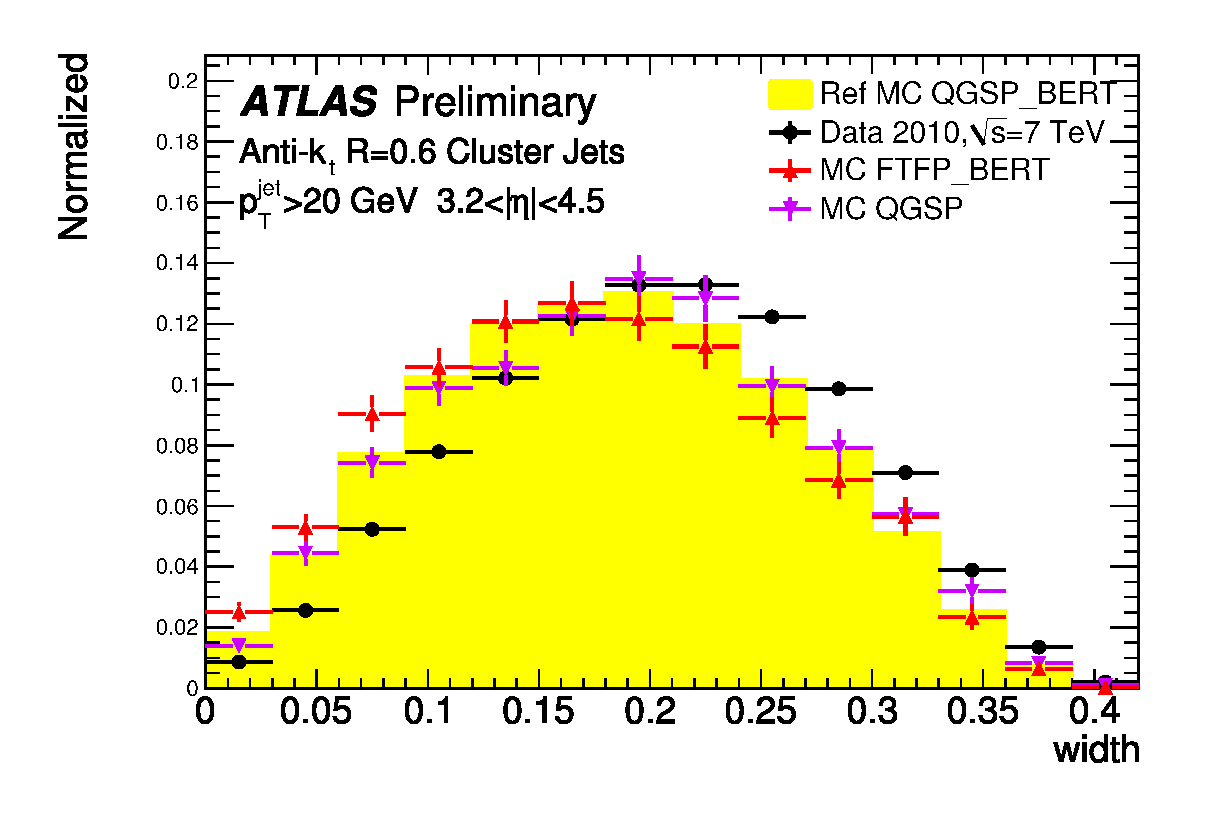
\includegraphics[width=\textwidth]{figures/JetPerformance/Width.eps}
        \end{subfigure}%
        \begin{subfigure}[b]{0.5\textwidth}
                \centering
                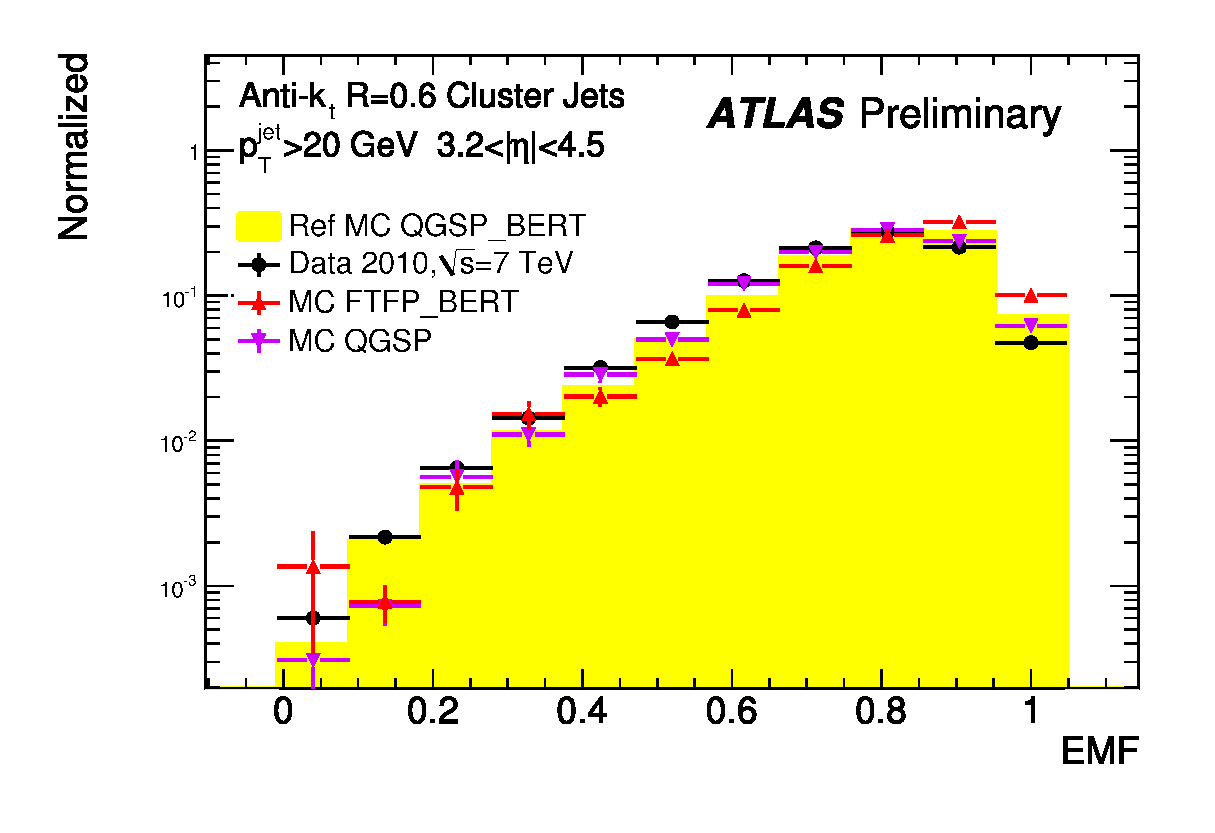
\includegraphics[width=\textwidth]{figures/JetPerformance/EMF.eps}
        \end{subfigure}%
\caption[Comparison of jet widths and EMF for data compared to PYTHIA with various physics lists]{
(a) Jet width and (b) jet EMF for jets with \pt{}$>20$ GeV and in the region \etaRange{3.2}{4.5}.
2010 data is compared to standard PYTHIA with the different physics lists, $\rm QGSP\textunderscore{}BERT$ (yellow filled), $\rm FTFP\textunderscore{}BERT$ (red circles) and $\rm QGSP$ (purple circles).  
\label{JetPerf:Width_EMF}}
\end{figure}


%
%

\chapter{Measurement of Dijet Production with a Veto on Additional Central Jet Activity}
\label{chp:GBJ1}
The study into dijet production with a jet veto is presented.
These observables are compared for a dijet rapidity separation of up to 6 units in rapidity, and $50\le\ptb{}<500$.
The data are compared to POWHEG with both the PYTHIA parton shower (POWHEG + PYTHIA) and the HERWIG parton shower (POWHEG + HERWIG), and also to the HEJ generator. 
The data are also compared to PYTHIA, HERWIG++ and ALPGEN.
A description of these genertors can be found in Section \ref{Theory:MC}.

The topology and event selection are outlined in Section \ref{sec:GBJ1:AnalSel} and \ref{sec:GBJ1:EvtSel}, respectively. 
In Section \ref{sec:GBJ1:DataStab}, the robustness of the event selection will be examined. 
In Section \ref{sec:GBJ1:Uncorr}, the selected data will be compared to the simulated PYTHIA sample.
Section \ref{sec:GBJ1:OtherWork} outlines the work done by other members of the analysis team that was required to get the final measurements, which are presented in Section \ref{sec:GBJ1:FinalPlots} and published in \cite{ATLASGap}. 

%-introduction to the analysis
%   -define why we look at it
%   -what observables we want to look at
%
%-give a bit of info on what is going to be in each chapter

\section{Topology Selection}
\label{sec:GBJ1:AnalSel}
The jets used in this analysis were reconstructed using the anti$-k_T$ algorithm with a radius parameter R=0.6\footnote{The anti$-k_T$ algorithm is described in Section XXX}. 
Only jets that have \pt{}$>20$ GeV and $|y|<4.4$ have been used, as these are the regions that have a well defined jet energy scale and jet cleaning cuts. 


The analysis uses two different dijet selection criteria, ``Leading \pt{} Dijet Selection" and ``Forward/Backward Selection", to define two boundary jets. 

In the leading dijet \pt{} selection the boundary jets are the two highest \pt{} jets in the event, and in the forward/backward selection the two boundary jets are the most forward (positive rapidity) and most backward (negative rapidity) jet in the event. 



Once the boundary jets have been assigned, an additional cut is applied to the average transverse momentum, \ptb{},of the boundary jets of 50 GeV. 
The \ptb{} cut is required to ensure that the event is in a high efficiency trigger region. 
These cuts define the inclusive events for the analysis. 


To study the activity in the rapidity region between the boundary jets, two variables are investigated. 
The first is the ``Gap Fraction". This is the fraction of the inclusive sample  that passes a jet veto, which excludes events that have an additional jet with \pt{} greater than the jet veto scale,\qz{}, in the dijets rapidity region. 
The gap fraction, \gap, is defined by,
\begin{equation}
f_{\rm gap} = \frac{n (\qz{})}{N},
\label{GBJ1:fgap}
\end{equation}
where n(\qz{}) is the number of gap events, events which pass the jet veto, and $N$ is the inclusive number of events.
The nominal choice of the jet veto scale is \qz{}$=20$ GeV. 

The second variable studied is the mean number of jets, which have \pt{}$>$\qz{}, in the dijet rapidity region, ie 
\begin{equation}
\nb{} = 
\label{GBJ1:fgap}
\end{equation}
where ....

*Now discuss some errors*

\section {Event selection}
\label{sec:GBJ2:EvtSel}
\subsection{Data Samples and Basic Event Selection}
The analysis was performed using pp colisions at $\sqrt{s}=7$ TeV, recorded between April and October 2010 using the ATLAS detector with an unprescaled luminosity of XXXXX.
Stable beam conditions and good data quality was required for the data used; the data quality was assessed by checking that all the parts of the detector and trigger were performing normally, and the physics objects (eg jets and muons) were being correctly reconstructed. 

Jets were required to have two jets with $\pt{}>20 $ GeV with $|y|<4.4$.
Events are rejected if there is any jet with $p_T>20$ GeV which is found as either bad or ugly as described in Section \ref{sec:GBJ1:Noise_Pileup}. 
Events are also rejected if the number of reconstructed primary vertices is not equal to one.


\subsection{Trigger Strategy}

For each of the two leading offline jets, a specific trigger chain is assigned depending on the rapidity, $y$, and \pt{} of the offline jet as well as the run number the event occured in.
Tables \ref{tab:CentralTrigger}, \ref{tab:TransTrigger} and \ref{tab:ForwardTrigger} show the trigger chains used in central ($|y_{jet}|<2.9$), forward transition ($3.3\le|y_{jet}|<3.6$) and forward trigger regions ($3.6\le|y_{jet}|<4.4$) respectively.
If a jet falls into the region $2.9\le|y_{jet}|<3.3$, the offline jet is matched to the closest level one trigger jet using $\dr{}=\sqrt{\dphi{}^2 + \deta{}^2}$.
It is defined as a central (forward) jet  if it is closest to a trigger jet that fired a central (forward) jet trigger, and a trigger chain is deturmined using Table \ref{tab:CentralTrigger} (Table \ref{tab:TransTrigger}).
Either of the trigger chains assosiated with the leading jets are required to fire for the event to pass.

This trigger strategy has previously been used in the measurement of te dijet cross section \cite{ref:Dijet}.
In most region of phase spcae, the trigger efficiency for each considered jet is $100\%$ efficient.
However, there are two regions where that is not the case.
The first is the crack region, $1.3\le|y_{jet}|\le1.6$, between the barrel and end-cap calorimeter.
The second is in the positive FCAL region in which there is a dead trigger tower that reduces the trigger efficiency for jets with $|y_{jet}|>3.1$.
For each jet that fills in one of these regions, the event is weighted by 
\begin{equation}
W_{eff}= \frac{\mathcal{P}_{lead}}{\epsilon_{lead}} + \frac{\mathcal{P}_{sublead}}{\epsilon_{sublead}} -\frac{\mathcal{P}_{lead}\mathcal{P}_{sublead}}{\epsilon_{lead}\epsilon_{sublead}}
\label{GBJ2:Eff}
\end{equation}
where $\mathcal{P}_{lead}$ and $\mathcal{P}_{sublead}$ is 1 if the event passed the leading and subleading trigger chain, else it is zero, and $\epsilon_{lead}$ and $\epsilon_{sublead}$ are the efficencies for the leading and subleading jets.

Prescales are applied to the trigger to preferencially select events with higher \pt{} jets, only the highest \pt{} trigger is unprescaled.
This results in a flattening of the jet \pt{} spectrum.
To retrive the original distribution the events are weighted by the inverse of an effective luminosity for each trigger combination.
By summing over the luminosity blocks, the  effective luminosity is calculated by
\begin{equation}
\mathcal{L}_{effective} = \sum_{LB} \frac{\mathcal{L}_{LB}}{P_{LB}^L P_{LB}^{SL}/(P_{LB}^L + P_{LB}^{SL} -1)}
\label{GBJ2:Eff}
\end{equation}
where $P_{LB}^L$ and $P_{LB}^{SL}$ are the prescales for a given luminosity for the trigger chain assosiated with the leading and subleading jet respectively, and $\mathcal{L}_{LB}$ is the luminosity for the luminosity block. 

The effective luminosities were calculated without the single vertex cut applied in this analysis. 
A single vertex correction is applied to the effective luminosity of every trigger combination which is the fraction of events with only one vertex. 

\begin{table}[htdp]
\centering
\begin{tabular}{ | c | c | c | c | }
  \hline
 \pt{} [GeV] & Period A-C & Period D-F & Period G-I \\
  \hline
20--42.5 &  $ \rm L1\_ MBTS\_ 1$ & $ \rm L1\_ MBTS\_ 1$ & $ \rm EF\_ mbMbts\_ 1\_ eff$  \\
42.5--70 &  $ \rm L1\_ J5$ &     $ \rm L1\_ J5$ &     $ \rm EF\_ j20\_ jetNoEF$  \\
70--97.5 &   $ \rm L1\_ J15$ &    $ \rm L1\_ J15$ &    $ \rm EF\_ j35\_ jetNoEF$  \\
97.5--152.5 &   $ \rm L1\_ J30$ &    $ \rm L1\_ J30$ &    $ \rm EF\_ j50\_ jetNoEF$  \\
152.5--197.5 &  $ \rm L1\_ J55$ &    $ \rm L1\_ J55$ &    $ \rm EF\_ j75\_ jetNoEF$  \\
197.5--217.5 &  $ \rm L1\_ J55$ &    $ \rm L1\_ J55$ &    $ \rm EF\_ j95\_ jetNoEF$  \\
217.5+ &     $ \rm L1\_ J55$ &    $ \rm L1\_ J55$ &    $ \rm EF\_ L1J95\_ NoAlg$ \\

  \hline
\end{tabular}
\caption{
Trigger chains used for central trigger region, $|y_{jet}|<2.9$, for jet \pt{} and period.
\label{tab:CentralTrigger}}
\end{table}%


\begin{table}[htdp]
\centering
\begin{tabular}{ | c | c | c | c | }
\hline
\pt{} [GeV] & Period A-D  & Period E-F & Period G-I \\
      \hline
         20--42.5 &     $ \rm L1\_ MBTS\_ 1$ & $ \rm L1\_ MBTS\_ 1$  &   $ \rm EF\_ mbMbts\_ 1\_ eff$  \\
         42.5--62.5 &   $ \rm L1\_ MBTS\_ 1$ & $ \rm L1\_ FJ10$      &   $ \rm EF\_ mbMbts\_ 1\_ eff$  \\
         62.5--72.5 &   $ \rm L1\_ MBTS\_ 1$ & $ \rm L1\_ FJ10$      &   $ \rm EF\_ fj30\_ jetNoEF$  \\
         72.5--95 &     $ \rm L1\_ MBTS\_ 1$ & $ \rm L1\_ FJ30$      &   $ \rm EF\_ fj30\_ jetNoEF$  \\
         95--160 &      $ \rm L1\_ MBTS\_ 1$ & $ \rm L1\_ FJ30$      &   $ \rm EF\_ fj50\_ jetNoEF$  \\
         160+ &         $ \rm L1\_ MBTS\_ 1$ & $ \rm L1\_ FJ30$      &   $ \rm EF\_ fj75\_ jetNoEF$  \\
         \hline
      \end{tabular}
      \caption{
      Trigger chains used for transition trigger region, $3.3\le|y_{jet}|<3.6$, for jet \pt{} and period.
      \label{tab:TransTrigger}}
\end{table}%

\begin{table}[htdp]
\centering
\begin{tabular}{ | c | c | c | c | }
  \hline
 \pt{} [GeV] & Period A-D & Period E-F & Period G-I \\
  \hline
20--42.5 &    $ L1\_ MBTS\_ 1$ & $ L1\_ FJ10$ & $ EF\_ mbMbts\_ 1\_ eff$  \\
42.5--50 &    $ L1\_ MBTS\_ 1$ & $ L1\_ FJ10$ & $ EF\_ fj30\_ jetNoEF$  \\
50--67.5 &    $ L1\_ MBTS\_ 1$ & $ L1\_ FJ30$ & $ EF\_ fj30\_ jetNoEF$  \\
67.5--100 &    $ L1\_ MBTS\_ 1$ & $ L1\_ FJ30$ & $ EF\_ fj50\_ jetNoEF$  \\
100+ &    $ L1\_ MBTS\_ 1$ & $ L1\_ FJ30$ & $ EF\_ fj75\_ jetNoEF$  \\

  \hline
\end{tabular}
\caption{
Trigger chains used for forward trigger region, $3.6\le|y_{jet}|<4.4$, for jet \pt{} and period.
\label{tab:ForwardTrigger}}
\end{table}%

 
% Why is comparing to uncorrected data important?

\section{Data compared to reconstructed PYTHIA }
\label{sec:GBJ1:Uncorr}
This section presents the data compared to the reconstructed PYTHIA sample, to check that the PYTHIA sample approximately agrees with data so that it can be used for unfolding the detecter effects in the data. 

Figures \ref{UncorrIncl_dy} - \ref{Uncorr_Pt3_dy} are various distributions with data and the reconstructed PYTHIA sample shown, and also the ratio between them.
Figure \ref{UncorrIncl_dy} shows the inclusive $\Delta y$ distribution for three different $\bar{p_T}$ slices. Figure \ref{Uncorr_Pt3_dy} shows the inclusive $p_T^{veto}$ distribution for two different slices in $\Delta y$ and $\bar{p_T}$ space. Figure \ref{Uncorr_GF} shows slices of the gap fraction against $\Delta y$ and $\bar{p_T}$.

The three figures show good agreement between the data and the reconstruted PYTHIA sample, and give confidence that the PYTHIA sample can be used for the unfolding factors. 

\begin{figure}
\centering
\mbox{
              \subfigure[]{\epsfig{figure=figures/GBJ1/UncorrectedData/Inclusive_selA_Ave_pT_70_90_Norm.eps,width=0.5\textwidth,height = 6cm}}\quad
              \subfigure[]{\epsfig{figure=figures/GBJ1/UncorrectedData/Inclusive_selA_Ave_pT_90_120_Norm.eps,width=0.5\textwidth,height = 6cm}}\quad
}
\mbox{
              \subfigure[]{\epsfig{figure=figures/GBJ1/UncorrectedData/Inclusive_selA_Ave_pT_180_210_Norm.eps,width=0.5\textwidth,height = 6cm}}\quad
                              }
\caption[Comparison between data and PYTHIA sample in the inclusive distribution for $\Delta y$]{
Fraction of events for each $\Delta y$ bin for 2010 uncorrected data and PYTHIA sample. Shown are (a) $70<\bar{p_T}<90$, (b) $90<\bar{p_T}<120$ and (c) $210<\bar{p_T}<240$ slices.
\label{UncorrIncl_dy}}
\end{figure}

\begin{figure}
\centering
\mbox{
              \subfigure[]{\epsfig{figure=figures/GBJ1/UncorrectedData/Pt3_dY_2_3_pt_90_120_PYTHIA.eps,width=0.5\textwidth,height = 6cm}}\quad
              \subfigure[]{\epsfig{figure=figures/GBJ1/UncorrectedData/Pt3_dY_2_3_pt_180_210_PYTHIA.eps,width=0.5\textwidth,height = 6cm}}\quad
                              }
\caption[Comparison between data and PYTHIA sample for Pt3 distribution]{Faction of events for each $p_T^{veto}$ bin for 2010 uncorrected data and PYTHIA sample. Shown are (a) $90<\bar{p_T}<120$ and $2 < \Delta y <3$, and (b) $90<\bar{p_T}<120$ and $2 < \Delta y <3$ slices.\label{Uncorr_Pt3_dy}}
\end{figure}

\begin{figure}
\centering
\mbox{
              \subfigure[]{\epsfig{figure=figures/GBJ1/UncorrectedData/RatioGF_selA_Ave_pT_90_120.eps,width=0.5\textwidth,height = 6cm}}\quad
              \subfigure[]{\epsfig{figure=figures/GBJ1/UncorrectedData/RatioGF_selA_DeltaY_2_3.eps,width=0.5\textwidth,height = 6cm}}\quad
                              }
\caption[Comparison of gap fraction between data and PYTHIA sample for $\Delta y$]{Gap fraction against (a) $\Delta y$ for the $90<\bar{p_T}<120$ slice and (b) $\bar{p_T}$ for the $2 < \Delta y <3$ slice, for 2010 uncorrected data and PYTHIA sample.\label{Uncorr_GF}}
\end{figure}



\section{Data Stability}
\label{sec:GBJ1:DataStab}

\subsection{Comparison between AOD and D3PD}
\label{sec:GBJ1:AODD3PD}

The cuts explained in section \ref{sec:GBJ1:EvtSel} were applied, and a cut flow was defined to check that there was stable running over the data and with the cuts. The analysis was done by both the author using the data in AOD format, and also independently by a different member of the analysis team running over D3PDs, which is a flat ntuple format. Table \ref{GBJ1:CutFlow} shows the number of events after each cut for both the AOD and D3PD formats, and also the fractional difference between the two, for the different data periods. The differences in the table are of the order 1:1000 which indicates that the cut flow is stable.  

   
\begin{table}
\small
\footnotesize

\begin{tabular}{|c|c|c|c|c|c|c|c|}
\hline
%
\input{figures/GBJ1/DataStability/AODD3PD/GBJCutFlow-Loose.csv}
%
\hline
\end{tabular}
\caption[Cut flow comparison between AOD and D3PD formats]{Cut flow comparison between AOD and D3PD formats for different data periods.}
\label{GBJ1:CutFlow}
\end{table}

\subsection{Jet Cleaning}
\label{sec:GBJ1:Cleaning}

The effect of jet cleaning is investigated by examining the change in the gap fraction and the inclusive distribution when using a tighter definition. 
Figure \ref{JetCleanIncl_dy} shows two slices in $\bar{p_T}$ of the inclusive distribution in $\Delta y$ with both the loose and medium cuts applied. 
There is $\thicksim\, 2\: \%\: $reduction in statistics using the medium cuts, but the shape of the distribution seems to be unchanged.  
The gap fraction is shown as a function of $\bar{p_T}$ in figure \ref{JetCleanGF_dy} and as a function of $\Delta y$ in figure \ref{JetCleanGF_pt} with the two different jet cleaning definitions. 
The difference in the gap fraction between the two cleaning definitions is small ($<1\%$) and within the statistical uncertainty of the samples, and as more statistics are gained with the loose bad jet definition, this is used for the remaining analysis. 

*add in more plots including the average jets in the gap*

\begin{figure}
\centering
\mbox{
              \subfigure[]{\epsfig{figure=figures/GBJ1/JetCleaning/Inclusive_selA_Ave_pT_90_120.eps,width=0.5\textwidth,height = 6cm}}\quad
              \subfigure[]{\epsfig{figure=figures/GBJ1/JetCleaning/Inclusive_selA_Ave_pT_210_240.eps,width=0.5\textwidth,height = 6cm}}\quad
                              }
\caption[Effect of jet cleaning on the inclusive distribution for $\bar{p_T}$]{Number of events for each $\Delta y$ bin for medium and loose jet cleaning definitions. Shown are (a) $90<\bar{p_T}<120$ and (b)$210<\bar{p_T}<240$ slices.\label{JetCleanIncl_dy}}
\end{figure}

\begin{figure}
\centering
\mbox{
              \subfigure[]{\epsfig{figure=figures/GBJ1/JetCleaning/RatioGF_selA_Ave_pT_90_120.eps,width=0.5\textwidth,height = 6cm}}\quad
              \subfigure[]{\epsfig{figure=figures/GBJ1/JetCleaning/RatioGF_selA_Ave_pT_210_240.eps,width=0.5\textwidth,height = 6cm}}\quad
                              }
\caption[Effect of jet cleaning on the gap fraction for $\bar{p_T}$]{Gap fraction for each $\Delta y$ bin for medium and loose jet cleaning definitions. Shown are (a) $90<\bar{p_T}<120$ and (b)$210<\bar{p_T}<240$ slices.\label{JetCleanGF_dy}}
\end{figure}


\begin{figure}
\centering
\mbox{
              \subfigure[]{\epsfig{figure=figures/GBJ1/JetCleaning/RatioGF_selA_DeltaY_1_2.eps,width=0.5\textwidth,height = 6cm}}\quad
              \subfigure[]{\epsfig{figure=figures/GBJ1/JetCleaning/RatioGF_selA_DeltaY_3_4.eps,width=0.5\textwidth,height = 6cm}}\quad
                              }
\caption[Effect of jet cleaning on the gap fraction for $\Delta y$]{Gap fraction for each $\bar{p_T}$ bin for medium and loose jet cleaning definitions. Shown are (a) $1<\Delta y<2$ and (b) $3<\Delta y<4$ slices.\label{JetCleanGF_pt}}
\end{figure}


% Jet Moments: https://twiki.cern.ch/twiki/bin/viewauth/AtlasProtected/JetMomentsForBadCells
% How to clean jets: https://twiki.cern.ch/twiki/bin/viewauth/AtlasProtected/HowToCleanJets
% Ugly Jets:
%           neighbour average correction: https://twiki.cern.ch/twiki/bin/viewauth/AtlasProtected/DeadCellCorrection


% Talks on bad jets : 
%           https://indico.cern.ch/getFile.py/access?contribId=2&resId=1&materialId=slides&confId=102852
%           https://indico.cern.ch/getFile.py/access?contribId=1&resId=1&materialId=slides&confId=102862


\subsection{Pile-up}
\label{sec:GBJ1:Pileup}



Two effects from pile-up are studied; in-time pile-up and out-of-time (OOT) pile-up.
In-time pile-up is additional proton-proton interactions in the event and is dependent on the number of primary vertices in the event.
Out-of-time pile-up is additional energy coming from previous bunch collisions and depends on both the number of primary vertices of the previous bunches and the bunch spacing. 
Both have the effect of adding additional energy into the event, which can affect the gap fraction.

The cut requiring one primary vertex will reduce the effect of in-time pile-up. 
The effect of the OOT pile-up and the residual in-time pile-up are assessed by comparing the average gap fraction for different pile-up conditions.
Table \ref{GBJ1:VertexAve} shows that the average number of primary vertices for different periods increases throughout 2010 data taking. 
The main changes in the bunch spacing are in period E where it was partially reduced and in period G where bunch trains, which had 150ns bunch spacing, were introduced.


The data periods are combined into two different bunch spacing conditions.
In periods B-D the bunch spacing was large, and so the effect of OOT pile-up is expected to be small.
In periods E-I, the bunch spacing was smaller, especially from period G onwards.
It is expected that the effect of OOT pile-up will be larger in this period.
The effect of OOT pile-up is assessed by considering the average gap fraction for different slices in \dy{} and \ptb{} as a function of data period.
The periods B-D and E-I are separately fitted with a horizontal line, and the differences between these fits are used to assess the effect. 

To assess the residual effect from in-time pile-up, the average gap fraction for different slices in \dy{} and \ptb{} as a function of data period is fitted with
\begin{equation}                              
y = A~\mathrm{and}~y = A + B x.
\label{GBJ1:Fit1}
\end{equation}
The first term has no period dependence, and the second has a period dependence.
For each function, the constants and the  $\chi^2/NDF$ are measured and assessed.
If there is no period dependence the period independent fit should do well, and the period dependent fit should have a zero gradient. 


Figures \ref{GBJ1:GFAve6070} - \ref{GBJ1:GFAve150180} show the average gap fraction as a function of period for various \dy{} and \ptb{} slices with fits to the two different OOT pile-up conditions, periods B-D and E-I, with a simple $y = A$ fit. 
Figure \ref{GBJ1:GFAve6070} shows this for a low \ptb{} range of 60--70 GeV for (a) $1<\dy{}<2$, (b) $2<\dy{}<3$ and (c) $3<\dy{}<5$.
The fit for the periods EFGHI is level with the period BCD for the lowest \dy{} range, $0.2$ above for the medium \dy{} range and $0.1$ below for the \dy{} range.
For this \ptb{} range no trend is observed.
Figures \ref{GBJ1:GFAve90120} and \ref{GBJ1:GFAve150180} show a similar lack of trend and difference within $0.2$.
These results would indicate that there is no significant effect from OOT pile-up. 


Table \ref{GBJ1:GFAveTable} shows the result of all the fits for the various \dy{} and \ptb{} slices. 
The $\chi^2/NDF$ of the period-independent fit show that the fits have good agreement with a straight line with no period dependence.
The period-dependent fit show the gradient of the line, $B$, is consistent, within statistical errors, with zero for almost all slices. 


These two methods have shown that after the primary vertex cut, the effect of pile-up is negligible, especially when compared to the systematic uncertainties discussed later. 
 
\begin{table}
\begin{center}
\begin{tabular}{|c|c|}
\hline
Period&Ave $N^o$ Vertices\\
\hline
B&1.07\\
C&1.06\\
D&1.57\\
E&1.89\\
F&2.18\\
G&2.46\\
H&2.33\\
I&2.78\\
\hline
\end{tabular}
\caption[Average number of primary vertices for different data periods]{ 
Average number of vertices for the different data taking periods.
\label{GBJ1:VertexAve}}
\end{center}
\end{table}

\begin{figure}
\centering
\mbox{
              \subfigure[]{\epsfig{figure=figures/GBJ1/DataStability/Pileup/GFAve_060_70_1-2_exclusive.eps,width=0.5\textwidth}}\quad
              \subfigure[]{\epsfig{figure=figures/GBJ1/DataStability/Pileup/GFAve_060_70_2-3_exclusive.eps,width=0.5\textwidth}}\quad
}
\mbox{

              \subfigure[]{\epsfig{figure=figures/GBJ1/DataStability/Pileup/GFAve_060_70_3-5_exclusive.eps,width=0.5\textwidth}}\quad
                              }
\caption[Average gap fraction versus period for $60<\ptb{}<70$ GeV]{
Average gap fraction with $60<\ptb{}<70$ GeV and (a) $1<\dy{}<2$, (b) $2<\dy{}<3$  and (c) $3<\dy{}<5$. 
Each set of average gap fractions have been fitted with three horizontal lines; one for periods B-D, one for periods E-I and one for all periods.
\label{GBJ1:GFAve6070}}
\end{figure}



\begin{figure}
\centering
\mbox{
              \subfigure[]{\epsfig{figure=figures/GBJ1/DataStability/Pileup/GFAve_090_120_1-2_exclusive.eps,width=0.5\textwidth}}\quad
              \subfigure[]{\epsfig{figure=figures/GBJ1/DataStability/Pileup/GFAve_090_120_2-3_exclusive.eps,width=0.5\textwidth}}\quad
}
\mbox{

              \subfigure[]{\epsfig{figure=figures/GBJ1/DataStability/Pileup/GFAve_090_120_3-5_exclusive.eps,width=0.5\textwidth}}\quad
                              }
\caption[Average gap fraction versus period for $90<\ptb{}<120$ GeV]{
Average gap fraction with $90<\ptb{}<120$ GeV and (a) $1<\dy{}<2$, (b) $2<\dy{}<3$  and (c) $3<\dy{}<5$. 
Each set of average gap fractions have been fitted with three horizontal lines; one for periods B-D, one for periods E-I and one for all periods.
\label{GBJ1:GFAve90120}}
\end{figure}



\begin{figure}
\centering
\mbox{
              \subfigure[]{\epsfig{figure=figures/GBJ1/DataStability/Pileup/GFAve_150_180_1-2_exclusive.eps,width=0.5\textwidth}}\quad
              \subfigure[]{\epsfig{figure=figures/GBJ1/DataStability/Pileup/GFAve_150_180_2-3_exclusive.eps,width=0.5\textwidth}}\quad
}
\mbox{

              \subfigure[]{\epsfig{figure=figures/GBJ1/DataStability/Pileup/GFAve_150_180_3-5_exclusive.eps,width=0.5\textwidth}}\quad
                              }
\caption[Average gap fraction versus period for $150<\ptb{}<180$ GeV]{
Average gap fraction with $150<\ptb{}<180$ GeV and (a) $1<\dy{}<2$, (b) $2<\dy{}<3$  and (c) $3<\dy{}<5$. 
Each set of average gap fractions have been fitted with three horizontal lines; one for periods B-D, one for periods E-I and one for all periods.
\label{GBJ1:GFAve150180}}
\end{figure}



\begin{table}
\footnotesize 
\centering
\begin{tabular}{ | c | c | c | c | c | c | c | c | }
\hline
\hline
\dy{} & \ptb{} & $\bar{f}_{gap}$&\multicolumn{2}{|c|}{$y = A$} & \multicolumn{3}{|c|}{y = A + Bx}\\
   & GeV& Periods B-D &A&$\chi^{2}$/NDF&A&B&$\chi^{2}$/NDF\\
%\dy{} & $\ptb{} [GeV]$ & $\bar{f}_{gap}$ & b & c & d & e & f  \\
\hline
\input{figures/GBJ1/DataStability/Pileup/AveGFTable2.txt}
\hline
\hline
\end{tabular}
\caption[Results from period dependent and period independent fits to the average gap fraction as a function of period]{
The results from the period dependent and period independent fits (Equation \ref{GBJ1:Fit1}) for various slices of \dy{} and \ptb{}.
\label{GBJ1:GFAveTable}}
\end{table}


\section{Overview of Other Analysis Components}
\label{sec:GBJ1:OtherWork}
To compare the data to theoretical models further aspects of the analysis were performed by other members of the analysis team. This section will dmension the unfolding of the data to hadron level. The systematic uncertainties in this analysis will then be discussed.

To compare the data to HEJ and POWHEG, detector and selection effects need to be accounted for, and the data needs to be unfolded back to hadron level. This was done using a bin-by-bin method comparing the final distributions from the PYTHIA sample at hadron and detector level. Rapidity weighted samples were generated and used to give good statistics in even the large $\Delta y$ regions.


The systematic uncertainties for various sources were considered. They were:
\begin{description}
\item[Jet Energy Scale (JES) uncertainty] varies depending on the $\Delta y$ bin. It can be as large at 5-10\% and is a significant source of uncertainty.

\item[Unfolding uncertainty] comes mainly from the limited statistics of the PYTHIA sample used to obtain the unfolding factors. It is a significant source of uncertainty with values as large as 5\%.

\item[Pileup] the effectiveness of the single primary vertex requirement, and the effect of out-of-time pileup was discussed in section \ref{sec:GBJ1:Pileup}. The average gap fraction was found to be unaffected by the change in pileup conditions, and so the effect from this is negligible.  

\item[Jet Cleaning Cuts] were changed to a stricter bad jet definition (which removed ~5\% of inclusive events) and there was a sub percent change to gap fraction distributions. This is negligble compared to the the uncertainty due to JES and unfolding.  

\item[Cosmic and beam backgrounds] event rates were estimated using triggers during non-filled bunch crossings. The rate of such evens was found to be very small compared to the rate of signal events, and the effect is taken to be negligible.

\item[Trigger Bias] was estimated by comparing the gap fraction and njets distributions with the analysis trigger strategy to the distributions obtained using the minimum bias stream and was found to be negligible in all regions.

\end{description}

The main two systematic uncertainties come from the JES and the unfolding. Figure \ref{GBJ1:SystUncert} shows the uncertainties from JES and unfolding and the combination for one $\Delta y$ and one $\bar{p_T}$ slice. The overall uncertainty does not change much with $\bar{p_T}$, but due to reduced statistics and moving into different regions of the detector both the JES, unfolding and overall uncertainty rise with larger $\Delta y$. For the final plots the overall systematic uncertainty and the statistical uncertainty have been added onto the data points.

\begin{figure}
\centering
\mbox{
              \subfigure[]{\epsfig{figure=figures/GBJ1/OtherWork/SystematicUncertainty_dY.eps,width=0.5\textwidth,height = 6cm}}\quad
              \subfigure[]{\epsfig{figure=figures/GBJ1/OtherWork/SystematicUncertainty_pT.eps,width=0.5\textwidth,height = 6cm}}\quad
                              }
\caption[Systematic uncertainty for the gap fraction for a slice in $\bar{p_T}$ and $\Delta y$]{Systematic uncertainty on the gap fraction versus (a) $\Delta y$ for $120<\bar{p_T}<150$ GeV and (b) $\bar{p_T}$ for $3<\Delta y<4$. 
\label{GBJ1:SystUncert}}
\end{figure}


\section{Final Plots}
\label{sec:GBJ1:FinalPlots}
In this section, the final plots that were shown in the publication are discussed. The plots shown are from  the leading $p_T$ dijet selection and the forward/backwards selection and show the gap fraction as a function of $\Delta y$, $\bar{p_T}$ and $Q_0$, and also the mean number of jets in the rapidity interval as a function of $\Delta y$ and $\bar{p_T}$. When $\Delta y$ and $\bar{p_T}$ is studied, $Q_0$ is always at a fixed value of 20 GeV. The data is sliced up into different regions, and so the gap fraction versus $\Delta y$ distribution is shown for seven different $\bar{p_T}$ ranges, and similarly for the $\bar{p_T}$ distribution. Each slice is offset to allow the data to be shown on one plot. The ratio of the theory predictions to data is shown next to each plot.

On each plot, the black points are the data points with statistical uncertainty bars, with the yellow bands indicating the systematic uncertainty from both the JES and unfolding. The red and blue dotted lines are the POWHEG + PYTHIA and POWHEG + HERWIG predictions respectively, and the blue band is the HEJ prediction with a theoretical uncertainty.

Figures \ref{GBJ1:dYSelA} and \ref{GBJ1:pTSelA} show the gap fraction as a function of $\Delta y$ and $\bar{p_T}$ respectively. These figures illustrate that HEJ  agrees well with the data for the complete range in $\Delta y$ for low $\bar{p_T}$, but at higher $\bar{p_T}$ slices it seems to deviate away from the data giving too many gap events. As explained in section XXX, HEJ works by resumming terms of $\Delta y$, but has no resummation when $\bar{p_T}>>Q_0$. It is, therefore not too surprising that a deviation if observed at larger $\bar{p_T}/Q_0$ ($Q_0$ is fixed). 
POWHEG + PYTHIA probably gives the best overall description of the data, but at large $\Delta y$ the gap fraction is too low. *explain why this might be for POWHEG in general*  POWHEG + HERWIG seems to give too much activity in all phase space regions, and this deviation becomes larger for larger $\Delta y$. 


%Figures \ref{GBJ1:dYSelA} and \ref{GBJ1:pTSelA} are the gap fraction as a function of $\Delta y$ and $\bar{p_T}$ respectively. Figure \ref{GBJ1:dYSelA} illistrates that for low $\bar{p_T}$ that HEJ agrees well with the data for the complete range in $\Delta y$, but at higher $\bar{p_T}$ slices it seems to deviate away from the data. The figure also shows how both POWHEG curves agree at low $\Delta y$, but deviates at higher $\Delta y$. Figure \ref{GBJ1:pTSelA} makes this point even more apparent where POWHEG + PYTHIA agrees well with the data accross the $\bar{p_T}$ range for low $\Delta y$ slices, but then deviates in the larger $\Delta y$ slices.


Figure \ref{GBJ1:Q0SelA} is the gap fraction as a function of $Q_0$ for various $\Delta y$ and $\bar{p_T}$ slices. The figure shows that none of the theoretical curves agree well with the data when the large $\Delta y$ or $\bar{p_T}$ slices are considered. Both HEJ and POWHEG + PYTHIA do well in the low $\Delta y$ and $\bar{p_T}$ slice. At larger $\Delta y$ and $\bar{p_T}$ slices they both deviate from the data, with HEJ improving its agreement at larger values of $Q_0$. As seen in the previous figures, POWHEG + HERWIG still gives a gap fraction lower than the POWHEG + PYTHIA, and that is far from the data for all ranges. 


%Figure \ref{GBJ1:Q0SelA} is the gap fraction as a function of $Q_0$ for various $\Delta y$ and $\bar{p_T}$ slices. The figure shows that the POWHEG + PYTHIA agrees with the data quite well for the low $\Delta y$ slices (even with a larger $\bar{p_T}$ slice), but seems to undershots the data for the larger $\Delta y$ slices, indicating that there is not enough activity in the gap region for large $\Delta y$ events. HEJ doesn quite well in the low $\Delta y$ and low $\bar{p_T}$ slice, but overshots at low $Q_0$ at either larger $\Delta y$ or $\bar{p_T}$ slices, indicating that events are two likely to have a jet with $p_T>20$ GeV in all events bar the low  $\Delta y$ or $\bar{p_T}$ region.


Figures \ref{GBJ1:NjetsdYSelA} and \ref{GBJ1:NjetspTSelA} are the mean number of jets in the rapidity interval between the boundary jets as a function of $\Delta y$ and $\bar{p_T}$ respectively. This is an alternative method of probing the activity between the boundary jets. The gap fraction is only concerned with the leading jet in the rapidity region, but the average number of jets considers all jet in that region with a $p_T>20$ GeV. In both plots it can be seen that, except at very low $\bar{p_T}$, HEJ underestimates the the number of jets in the gap region, which is in agreement with what is seen in the gap fraction plots. POWHEG + PYTHIA agrees well  with the data in all regions and it is still the best descriptor of the data, whereas POWHEG + HERWIG seems to slightly overestimate the data, and gets worse at lower $\bar{p_T}$.  

%Figures \ref{GBJ1:NjetsdYSelA} and \ref{GBJ1:NjetspTSelA} are the mean number of jets in the rapidity interval between the boundary jets as a function of $\Delta y$ and $\bar{p_T}$ respectively. In both plots it can be seen that, except at very low $\bar{p_T}$, HEJ underestimates the the number of jets in the gap region. POWHEG + PYTHIA does quite well in all regions of agreeing with the data, whereas POWHEG + HERWIG seems to slightly overestimate the data thorught the curves.  
 
*I intend to also talk about the Selection B stuff, but there is a lot of it, and I think I will need to discuss how much will go in, and also a chat with Andy to fully understand what we see in all the plots.*


Since publishing the results of this analysis, several papers [reference Simones and Jeppes here] have compared  their theoretical predictions to the ATLAS data. 
Reference [Jeppe] commented on the ATLAS data, coming to similar conclusions to our paper. They then went on to investigate when fixed order calculations become unreliable in this topology of event.
Reference [Simones] used an all-order resummation in $\log\frac{\bar{p_T}}{Q_0}$ terms to compare to the data. After matching to 2$\rightarrow$3 matrix element, the results agreed very well with the data in both the gap fraction versus $Q_0$ and  $\Delta y$, coming to their stated conclusion that: ``The message is clear: the accuracy of the ATLAS data already demands better theoretical calculations."

*Here do I want to start leading in to the next chapter by stating the reason we continued looking at this? or should I save that for the intro to next chapter?*


\begin{figure}
\centering
\mbox{
              \subfigure[]{\epsfig{figure=figures/GBJ1/FinalData/GF_dY.eps,width=0.5\textwidth}}\quad
              \subfigure[]{\epsfig{figure=figures/GBJ1/FinalData/GF_dY_ratio.eps,width=0.5\textwidth}}\quad
}
\caption[Gap fraction as a function of $\Delta y$ for leading $p_T$ dijet selection]{ (a) Gap fraction as a function of $\Delta y$ for various $\bar{p_T}$ slices. (b) Ratio between the theoretical predictions and data. Leading $\bar{p_T}$ dijet selection.
\label{GBJ1:dYSelA}}
\end{figure}



\begin{figure}
\centering
\mbox{
              \subfigure[]{\epsfig{figure=figures/GBJ1/FinalData/GF_ptBar.eps,width=0.5\textwidth}}\quad
              \subfigure[]{\epsfig{figure=figures/GBJ1/FinalData/GF_ptBar_ratio.eps,width=0.5\textwidth}}\quad
}
\caption[Gap fraction as a function of $\bar{p_T}$ for leading $p_T$ dijet selection]{ (a) Gap fraction as a function of $\bar{p_T}$ for various $\Delta y$ slices. (b) Ratio between the theoretical predictions and data. Leading $\bar{p_T}$ dijet selection.
\label{GBJ1:pTSelA}}
\end{figure}



\begin{figure}
\centering
\mbox{
              \subfigure[]{\epsfig{figure=figures/GBJ1/FinalData/GF_Q0.eps,width=0.5\textwidth}}\quad
              \subfigure[]{\epsfig{figure=figures/GBJ1/FinalData/GF_Q0_ratio.eps,width=0.5\textwidth}}\quad
}
\caption[Gap fraction as a function of $Q_0$ for leading $p_T$ dijet selection]{ (a) Gap fraction as a function of $Q_0$ for various $\Delta y$ and $\bar{p_T}$ slices. (b) Ratio between the theoretical predictions and data. Leading $\bar{p_T}$ dijet selection.
\label{GBJ1:Q0SelA}}
\end{figure}

\begin{figure}
\centering
\mbox{
              \subfigure[]{\epsfig{figure=figures/GBJ1/FinalData/GF_Njets_dY.eps,width=0.5\textwidth}}\quad
              \subfigure[]{\epsfig{figure=figures/GBJ1/FinalData/GF_Njets_dY_ratio.eps,width=0.5\textwidth}}\quad
}
\caption[Mean number of jets as a function of $\Delta y$ for leading $p_T$ dijet selection]{ (a) Mean number of jets as a function of $\Delta y$ for various $\bar{p_T}$ slices. (b) Ratio between the theoretical predictions and data. Leading $\bar{p_T}$ dijet selection.
\label{GBJ1:NjetsdYSelA}}
\end{figure}

\begin{figure}
\centering
\mbox{
              \subfigure[]{\epsfig{figure=figures/GBJ1/FinalData/GF_Njets.eps,width=0.5\textwidth}}\quad
              \subfigure[]{\epsfig{figure=figures/GBJ1/FinalData/GF_Njets_ratio.eps,width=0.5\textwidth}}\quad
}
\caption[Mean number of jets as a function of $\bar{p_T}$ for leading $p_T$ dijet selection]{ (a) Mean number of jets as a function of $\bar{p_T}$ for various $\Delta y$ slices. (b) Ratio between the theoretical predictions and data. Leading $\bar{p_T}$ dijet selection.
\label{GBJ1:NjetspTSelA}}
\end{figure}

%%%%%%%%%%%%%%%%%%%SELECTION B%%%%%%%%%%%%%%%%%%%%%%

\begin{figure}
\centering
\mbox{
              \subfigure[]{\epsfig{figure=figures/GBJ1/FinalData/GF_dY_SelB.eps,width=0.5\textwidth}}\quad
              \subfigure[]{\epsfig{figure=figures/GBJ1/FinalData/GF_dY_SelB_ratio.eps,width=0.5\textwidth}}\quad
}
\caption[Gap fraction as a function of $\Delta y$ for forward backward selection]{ (a) Gap fraction as a function of $\Delta y$ for various $\bar{p_T}$ slices. (b) Ratio between the theoretical predictions and data. Forward backward selection.
\label{GBJ1:dYSelB}}
\end{figure}

\begin{figure}
\centering
\mbox{
              \subfigure[]{\epsfig{figure=figures/GBJ1/FinalData/GF_SelB_pT.eps,width=0.5\textwidth}}\quad
              \subfigure[]{\epsfig{figure=figures/GBJ1/FinalData/GF_SelB_pT_ratio.eps,width=0.5\textwidth}}\quad
}
\caption[Gap fraction as a function of $\bar{p_T}$ for forward backward selection]{ (a) Gap fraction as a function of $\bar{p_T}$ for various $\Delta y$ slices. (b) Ratio between the theoretical predictions and data. Forward backward selection.
\label{GBJ1:pTSelB}}
\end{figure}

\begin{figure}
\centering
\mbox{
              \subfigure[]{\epsfig{figure=figures/GBJ1/FinalData/GF_SelB_Q0.eps,width=0.5\textwidth}}\quad
              \subfigure[]{\epsfig{figure=figures/GBJ1/FinalData/GF_SelB_Q0_ratio.eps,width=0.5\textwidth}}\quad
}
\caption[Gap fraction as a function of $Q_0$ for forward backward selection]{ (a) Gap fraction as a function of $Q_0$ for various $\Delta y$ and $\bar{p_T}$ slices. (b) Ratio between the theoretical predictions and data. Forward backward selection.
\label{GBJ1:Q0SelB}}
\end{figure}


\begin{figure}
\centering
\mbox{
              \subfigure[]{\epsfig{figure=figures/GBJ1/FinalData/Njets_SelB_dY.eps,width=0.5\textwidth}}\quad
              \subfigure[]{\epsfig{figure=figures/GBJ1/FinalData/Njets_SelB_dY_ratio.eps,width=0.5\textwidth}}\quad
}
\caption[Mean number of jets as a function of $\Delta y$ for forward backward selection ]{ (a) Mean number of jets in rapidity region as a function of $\Delta y$ for various $\bar{p_T}$ slices. (b) Ratio between the theoretical predictions and data. Forward backward selection.
\label{GBJ1:nJetsdYSelB}}
\end{figure}

\begin{figure}
\centering
\mbox{
              \subfigure[]{\epsfig{figure=figures/GBJ1/FinalData/Njets_SelB_pT.eps,width=0.5\textwidth}}\quad
              \subfigure[]{\epsfig{figure=figures/GBJ1/FinalData/Njets_SelB_pT_ratio.eps,width=0.5\textwidth}}\quad
}
\caption[Mean number of jets as a function of $\Delta y$ for forward backward selection]{ (a) Mean number of jets in rapidity region as a function of $\bar{p_T}$ for various $\Delta y$ slices. (b) Ratio between the theoretical predictions and data. Forward backward selection.
\label{GBJ1:nJetspTSelB}}
\end{figure}


\begin{figure}
\centering
\mbox{
              \subfigure[]{\epsfig{figure=figures/GBJ1/FinalData/Njets_SelB_dY_Q0pTbar.eps,width=0.5\textwidth}}\quad
              \subfigure[]{\epsfig{figure=figures/GBJ1/FinalData/Njets_SelB_dY_Q0pTbar_ratio.eps,width=0.5\textwidth}}\quad
}
\caption[Gap fraction as a function of $\Delta y$ for forward backward selection and variable $Q_0$]{ (a) Gap fraction as a function of $\Delta y$ for various $\bar{p_T}$ slices. (b) Ratio between the theoretical predictions and data. Forward backward selection with veto scale set as $\bar{p_T}$.
\label{GBJ1:pTSelB}}
\end{figure}



%\begin{figure}[h]
%\centering
%
%        \begin{subfigure}[b]{0.45\textwidth}
%                \centering
%                \epsfig{figure=figures/GBJ1/FinalData/GF_dY.eps,width=\textwidth}
%
%                \caption[hang]{A gull}
%                \label{fig:gull}
%        \end{subfigure}%
%        \begin{subfigure}[b]{0.45\textwidth}
%                \centering
%                \epsfig{figure=figures/GBJ1/FinalData/GF_dY_ratio.eps,width=\textwidth}
%                                \vspace{-1cm}
%
%                \caption{A tiger}
%                \label{fig:tiger}
%        \end{subfigure}
%        
%         \begin{subfigure}[b]{0.45\textwidth}
%                \centering
%                \epsfig{figure=figures/GBJ1/FinalData/GF_dY.eps,width=\textwidth}
%                                \vspace{-1cm}
%
%                \caption{A gull}
%                \label{fig:gull}
%        \end{subfigure}%
%        \begin{subfigure}[b]{0.45\textwidth}
%                \centering
%                \epsfig{figure=figures/GBJ1/FinalData/GF_dY_ratio.eps,width=\textwidth}
%                                \vspace{-1cm}
%
%                \caption{A tiger}
%                \label{fig:tiger}
%        \end{subfigure}
%         \caption{This is a large caption for my figures to see where it will be placed.}
%
%\end{figure}


%\chapter{Dijets with a Jet Veto and Azimuthal Decorrelations at Very Large Rapidity Separations}
%\label{chp:GBJ2}
%The first LHC measurement of dijet production with a jet veto (documented in Chapter \ref{chp:GBJ1} and \cite{ref:ATLASGap}) examined the gap fraction in slices \ptb{} up to $\dy{}=6$.
This cut-off in \dy{} was necessary because the analysis used a central jet trigger strategy in which the trigger fired if a jet was within $|y|<2.8$.
There was a relatively small number of events at large \dy{} and where the statistical uncertainties were large. 
The data was compared to state of the art theory predictions by HEJ and POWHEG.
Whilst the HEJ curves described the with data as a function of \dy{}, the POWHEG curves did not.

The analysis was extended to probe the gap fraction at large \dy{} region.
The large \dy{} region is again studied using the 2010 data, but using a new dijet trigger strategy that allowed measurements up to $\dy{}=8$, which is the limit of the detector.
In addition, the effect of quark/gluon emission from the dijet system is studied using the azimuthal decorrelation between the jets that make up the dijet system.
The previous ATLAS measurement of azimuthal decorrelation, \cite{ref:Decorr}, was carried out using jets with an $\eta{} < 0.8$.


%\section{Topology Selection}
\label{sec:GBJ2:AnalSel}
The jets used in this analysis were reconstructed from EM scale calorimeter clusters with the anti$-k_T$ algorithm, described in Section \ref{sec:Theory:Jets}, using a radius parameter R=0.6.
As for the previous analysis, jets that have \pt{}$>20$ GeV and $|y|<4.4$ are used, as these have a well defined jet energy scale and jet cleaning cuts.
The dijet system is defined by the two leading jets in the event, with cuts on the transverse momentum of the leading and sub-leading jets of $\pt{}>60$ GeV and $\pt{}>50$ GeV, respectively.



The observables studied can loosely be divided into azimuthal decorrelation observables, and jet veto observables.
The jet veto observables are the same as defined in the previous chapter, where the gap fraction, \gap{}, is defined by,
\begin{equation}
f_{\rm gap} = \frac{N (\qz{})}{N},
\label{GBJ2:fgap}
\end{equation}
where N(\qz{}) is the number of gap events that do not contain a jet with $\pt{}>\qz{}$ in the rapidity interval between the boundary jets and $N$ is the inclusive number of events.
The gap fraction is studied as a function of \dy{} and \qz{}.
Again the mean number of jets, \nb{}, found in the rapidity region between the dijets that have \pt{}$>$\qz{} is also studied. 
The azimuthal decorrelation variables are
\begin{equation}
\frac{d\sigma}{d\Delta\phi},~\mean{\cosdphi}~\rm{and}~\mean{\costwodphi}.
\label{GBJ2:AZVar}
\end{equation}
The cross section as a function of \dphi{} is measured in slices of \dy{}.
The average decorrelation variables (\mean{\cosdphi} and \mean{\costwodphi})  are studied as a function of \dy{}.
All decorrelation variables are studied separately for inclusive and gap events (those that survived a jet veto).
The standard jet veto scale that is used to define gap events is $\qz{}=20$ GeV.



%\section {Event selection}
\label{sec:GBJ2:EvtSel}
\subsection{Data Samples and Basic Event Selection}
The analysis was performed using pp colisions at $\sqrt{s}=7$ TeV, recorded between April and October 2010 using the ATLAS detector with an unprescaled luminosity of XXXXX.
Stable beam conditions and good data quality was required for the data used; the data quality was assessed by checking that all the parts of the detector and trigger were performing normally, and the physics objects (eg jets and muons) were being correctly reconstructed. 

Jets were required to have two jets with $\pt{}>20 $ GeV with $|y|<4.4$.
Events are rejected if there is any jet with $p_T>20$ GeV which is found as either bad or ugly as described in Section \ref{sec:GBJ1:Noise_Pileup}. 
Events are also rejected if the number of reconstructed primary vertices is not equal to one.


\subsection{Trigger Strategy}

For each of the two leading offline jets, a specific trigger chain is assigned depending on the rapidity, $y$, and \pt{} of the offline jet as well as the run number the event occured in.
Tables \ref{tab:CentralTrigger}, \ref{tab:TransTrigger} and \ref{tab:ForwardTrigger} show the trigger chains used in central ($|y_{jet}|<2.9$), forward transition ($3.3\le|y_{jet}|<3.6$) and forward trigger regions ($3.6\le|y_{jet}|<4.4$) respectively.
If a jet falls into the region $2.9\le|y_{jet}|<3.3$, the offline jet is matched to the closest level one trigger jet using $\dr{}=\sqrt{\dphi{}^2 + \deta{}^2}$.
It is defined as a central (forward) jet  if it is closest to a trigger jet that fired a central (forward) jet trigger, and a trigger chain is deturmined using Table \ref{tab:CentralTrigger} (Table \ref{tab:TransTrigger}).
Either of the trigger chains assosiated with the leading jets are required to fire for the event to pass.

This trigger strategy has previously been used in the measurement of te dijet cross section \cite{ref:Dijet}.
In most region of phase spcae, the trigger efficiency for each considered jet is $100\%$ efficient.
However, there are two regions where that is not the case.
The first is the crack region, $1.3\le|y_{jet}|\le1.6$, between the barrel and end-cap calorimeter.
The second is in the positive FCAL region in which there is a dead trigger tower that reduces the trigger efficiency for jets with $|y_{jet}|>3.1$.
For each jet that fills in one of these regions, the event is weighted by 
\begin{equation}
W_{eff}= \frac{\mathcal{P}_{lead}}{\epsilon_{lead}} + \frac{\mathcal{P}_{sublead}}{\epsilon_{sublead}} -\frac{\mathcal{P}_{lead}\mathcal{P}_{sublead}}{\epsilon_{lead}\epsilon_{sublead}}
\label{GBJ2:Eff}
\end{equation}
where $\mathcal{P}_{lead}$ and $\mathcal{P}_{sublead}$ is 1 if the event passed the leading and subleading trigger chain, else it is zero, and $\epsilon_{lead}$ and $\epsilon_{sublead}$ are the efficencies for the leading and subleading jets.

Prescales are applied to the trigger to preferencially select events with higher \pt{} jets, only the highest \pt{} trigger is unprescaled.
This results in a flattening of the jet \pt{} spectrum.
To retrive the original distribution the events are weighted by the inverse of an effective luminosity for each trigger combination.
By summing over the luminosity blocks, the  effective luminosity is calculated by
\begin{equation}
\mathcal{L}_{effective} = \sum_{LB} \frac{\mathcal{L}_{LB}}{P_{LB}^L P_{LB}^{SL}/(P_{LB}^L + P_{LB}^{SL} -1)}
\label{GBJ2:Eff}
\end{equation}
where $P_{LB}^L$ and $P_{LB}^{SL}$ are the prescales for a given luminosity for the trigger chain assosiated with the leading and subleading jet respectively, and $\mathcal{L}_{LB}$ is the luminosity for the luminosity block. 

The effective luminosities were calculated without the single vertex cut applied in this analysis. 
A single vertex correction is applied to the effective luminosity of every trigger combination which is the fraction of events with only one vertex. 

\begin{table}[htdp]
\centering
\begin{tabular}{ | c | c | c | c | }
  \hline
 \pt{} [GeV] & Period A-C & Period D-F & Period G-I \\
  \hline
20--42.5 &  $ \rm L1\_ MBTS\_ 1$ & $ \rm L1\_ MBTS\_ 1$ & $ \rm EF\_ mbMbts\_ 1\_ eff$  \\
42.5--70 &  $ \rm L1\_ J5$ &     $ \rm L1\_ J5$ &     $ \rm EF\_ j20\_ jetNoEF$  \\
70--97.5 &   $ \rm L1\_ J15$ &    $ \rm L1\_ J15$ &    $ \rm EF\_ j35\_ jetNoEF$  \\
97.5--152.5 &   $ \rm L1\_ J30$ &    $ \rm L1\_ J30$ &    $ \rm EF\_ j50\_ jetNoEF$  \\
152.5--197.5 &  $ \rm L1\_ J55$ &    $ \rm L1\_ J55$ &    $ \rm EF\_ j75\_ jetNoEF$  \\
197.5--217.5 &  $ \rm L1\_ J55$ &    $ \rm L1\_ J55$ &    $ \rm EF\_ j95\_ jetNoEF$  \\
217.5+ &     $ \rm L1\_ J55$ &    $ \rm L1\_ J55$ &    $ \rm EF\_ L1J95\_ NoAlg$ \\

  \hline
\end{tabular}
\caption{
Trigger chains used for central trigger region, $|y_{jet}|<2.9$, for jet \pt{} and period.
\label{tab:CentralTrigger}}
\end{table}%


\begin{table}[htdp]
\centering
\begin{tabular}{ | c | c | c | c | }
\hline
\pt{} [GeV] & Period A-D  & Period E-F & Period G-I \\
      \hline
         20--42.5 &     $ \rm L1\_ MBTS\_ 1$ & $ \rm L1\_ MBTS\_ 1$  &   $ \rm EF\_ mbMbts\_ 1\_ eff$  \\
         42.5--62.5 &   $ \rm L1\_ MBTS\_ 1$ & $ \rm L1\_ FJ10$      &   $ \rm EF\_ mbMbts\_ 1\_ eff$  \\
         62.5--72.5 &   $ \rm L1\_ MBTS\_ 1$ & $ \rm L1\_ FJ10$      &   $ \rm EF\_ fj30\_ jetNoEF$  \\
         72.5--95 &     $ \rm L1\_ MBTS\_ 1$ & $ \rm L1\_ FJ30$      &   $ \rm EF\_ fj30\_ jetNoEF$  \\
         95--160 &      $ \rm L1\_ MBTS\_ 1$ & $ \rm L1\_ FJ30$      &   $ \rm EF\_ fj50\_ jetNoEF$  \\
         160+ &         $ \rm L1\_ MBTS\_ 1$ & $ \rm L1\_ FJ30$      &   $ \rm EF\_ fj75\_ jetNoEF$  \\
         \hline
      \end{tabular}
      \caption{
      Trigger chains used for transition trigger region, $3.3\le|y_{jet}|<3.6$, for jet \pt{} and period.
      \label{tab:TransTrigger}}
\end{table}%

\begin{table}[htdp]
\centering
\begin{tabular}{ | c | c | c | c | }
  \hline
 \pt{} [GeV] & Period A-D & Period E-F & Period G-I \\
  \hline
20--42.5 &    $ L1\_ MBTS\_ 1$ & $ L1\_ FJ10$ & $ EF\_ mbMbts\_ 1\_ eff$  \\
42.5--50 &    $ L1\_ MBTS\_ 1$ & $ L1\_ FJ10$ & $ EF\_ fj30\_ jetNoEF$  \\
50--67.5 &    $ L1\_ MBTS\_ 1$ & $ L1\_ FJ30$ & $ EF\_ fj30\_ jetNoEF$  \\
67.5--100 &    $ L1\_ MBTS\_ 1$ & $ L1\_ FJ30$ & $ EF\_ fj50\_ jetNoEF$  \\
100+ &    $ L1\_ MBTS\_ 1$ & $ L1\_ FJ30$ & $ EF\_ fj75\_ jetNoEF$  \\

  \hline
\end{tabular}
\caption{
Trigger chains used for forward trigger region, $3.6\le|y_{jet}|<4.4$, for jet \pt{} and period.
\label{tab:ForwardTrigger}}
\end{table}%

 
%\section{Closure of Event Selection}
\label{sec:GBJ2:AODD3PD}

To check the event selection, two separate implementations of the analysis were performed by the Manchester and UCL groups.
One of these analyses was carried out using the ATLAS AOD data format, whilst the other used the ATLAS D3PD format.
Figure \ref{GBJ2:AODD3PD:gap_njet} shows (a) the  gap fraction and (b) the  average number of jets in the rapidity region as a function of \dy{}.
Figure \ref{GBJ2:AODD3PD:dphi} shows the \dphi{} distribution for inclusive events for a dijet separation, \dy{}, of (a) 2-3 and (b) 4-5. 
All four plots show very good agreement between the AOD and D3PD implementations of the analysis.
The small disagreements arise from the data compression algorithms that store the data information.
This effects mainly the jet energies and the effect is much smaller than the JES uncertainty.


\begin{figure}
\centering
\mbox{
              \subfigure[]{\epsfig{figure=figures/GBJ2/AODD3PD/Comp_GapFraction_deltaY.eps,width=0.5\textwidth,height = 6cm}}\quad
              \subfigure[]{\epsfig{figure=figures/GBJ2/AODD3PD/Comp_prof_deltaY_njets.eps,width=0.5\textwidth,height = 6cm}}\quad
                              }
\caption[Comparison of gap fraction and mean number of jets between AOD data format and D3PD data format]{
(a) Gap fraction and (b) average number of jets in the rapidity region as a function of dijet separation, \dy{}, for 2010 uncorrected data from the AOD (red) and D3PD (black) data formats.
\label{GBJ2:AODD3PD:gap_njet}}
\end{figure}


\begin{figure}
\centering
\mbox{
              \subfigure[]{\epsfig{figure=figures/GBJ2/AODD3PD/Comp_dPhi__2_3-Edit.eps,width=0.5\textwidth,height = 6cm}}\quad
              \subfigure[]{\epsfig{figure=figures/GBJ2/AODD3PD/Comp_dPhi__4_5-Edit.eps,width=0.5\textwidth,height = 6cm}}\quad
                              }
\caption[Comparison of \dphiDist{} between AOD data format and D3PD data format]{
\dphiDist{} for inclusive events for a dijet separation of (a) $2<\dy{}<3$ and (b) $4<\dy{}<5$ for 2010 uncorrected data from the AOD (red) and D3PD (black) data formats.
\label{GBJ2:AODD3PD:dphi}}
\end{figure}


%\section{Systematic Uncertainty}
\label{GBJ2:system}

In this section, the systematic uncertainties from the jet cleaning cuts, jet energy scale uncertainty, jet energy resolution and jet $\phi$ resolution are assessed.
These uncertainties are added in quadrature with other uncertainties calculated by other members of the analysis team. 



%\subsection{Jet Energy Scale Uncertainty}

The effect of the JES is studied using the rapidity weighted PYTHIA samples.
Each jet, which is at the central value of the JES by default, is shifted up and down by $1 \sigma$ of the uncertainty of the JES.
The events are then passed through the event selection and three sets of the final distribution are made corresponding to nominal jets,  jets shifted up and jets shift down.
The shifted and nominal distributions were fitted by an appropriate distribution to reduce the fluctuations in the final JES uncertainty band.
The JES uncertainty band was found by taking the ratio of the shifted distribution (both up and down) to the nominal distribution.


********** Have a figure showing the JES uncertainty as a function of jet pt eta  ************

Figures \ref{GBJ2:JES:gap_njets} - \ref{GBJ2:JES:Q0} show the JES uncertainty bands for the final distributions.
The JES uncertainty shifting has two main effects that will apply differently in different distributions.
The first is shift the \pt{} of the leading jets which has the effect of moving events across the leading jets \pt{} cuts at 50 GeV and 60 GeV.
This results in more events for JES shifted up and less events for JES shifted down. 
The other effect is the shifting of the non-leading jets, the major effect is on the third jet \pt{} and this will effect the gap fraction distributions, or distributions that use gap events. 

The JES uncertainty band for the gap fraction as a function of \dy{} is shown in Figure \ref{GBJ2:JES:gap_njets} (a), and is small for low \dy{}, but increases at larger \dy{}.
The increase at larger \dy{} is due to the increase in the JES uncertainty at large \dy{}, causing large changes in the \pt{} of the non leading jets.
Figure \ref{GBJ2:JES:gap_njets} (b) shows the JES uncertainty band for the average number of jets in the rapidity region, and while there is some substructure, the overall uncertainty is approximately $\pm 10 \%$.
******Not sure yet on the shape of the njets*******


Figure \ref{GBJ2:JES:dPhi} shows the JES uncertainty bands for the \dphi{} distributions for both the inclusive and gap events, for the different \dy{} ranges.
The uncertainty bands for the \dphi{} distributions are significantly larger than for other distributions, because a shift in the JES can allow many more jets to pass the analysis \pt{} cuts and more events to enter the distributions.
The effect of the increase of events is smaller in the gap fraction which formed from a ratio and, as such, the increase in events effects both the numerator and denometer.
There is a slight increase in the JES uncertainty bands for smaller \dphi{} and for larger \dy{} regions the uncertainty bands increase.

The average \cosdphi{} and \costwodphi{} JES uncertainty bands are shown as a function of \dy{} in Figure \ref{GBJ2:JES:cos} (a) and (b) respectively. 
The JES uncertainty effects the inclusive events more than the gap events in both the distributions, and in the inclusive events the effect grows as a function of dijet rapidity separation.
The maximum effect of the JES uncertainty on the average \cosdphi{} is around $1\%$ for the inclusive events, and less than $0.5\%$ for the gap events.
For the average \costwodphi{} the effect from the JES uncertainty is around $3\%$ for the inclusive events, and less than $0.5\%$ for the gap events. 
********Think both inclusive shapes are prob due to the dphi of lower ptbar jets being closer to pi, but need to check*******

Figure \ref{GBJ2:JES:Q0} shows the JES uncertainty bands for the gap fraction as a function of the jet veto scale, \qz{}, for the \dy{} ranges 2--3, 4--5 and 7-8.
The uncertainty bands increase for larger \dy{}.
The uncertainty bands are largest at low \qz{} and reduce to zero for larger \qz{}.
At large values of \qz{} the gap fraction will be 1, and there are few jets with \pt{} close to \qz{}, and so the shifted third jet is unlikely to go above the \qz{} and change the gap fraction.
Conversely, at low \qz{} the gap fraction will not be 1, and there will be many jets with a \pt{} near the \qz{} cut, thus the shifted third jet \pt{}  can move across \qz{} changing the gap fraction.


\begin{figure}
\centering
\mbox{
              \subfigure[]{\epsfig{figure=figures/GBJ2/JES/Smeared__GapFraction_deltaY.eps,width=0.5\textwidth}}\quad
              \subfigure[]{\epsfig{figure=figures/GBJ2/JES/Smeared__prof_deltaY_njets.eps,width=0.5\textwidth}}\quad
                              }
\caption[]{
The uncertainty on the (a) gap fraction and (b) mean number of jets in the rapidity interval due to the JES uncertainty as a function of dijet rapidity separation. 
\label{GBJ2:JES:gap_njets}}
\end{figure}



\begin{figure}
\centering
\mbox{
              \subfigure[]{\epsfig{figure=figures/GBJ2/JES/Smeared__dPhi__7_8.eps,width=0.5\textwidth}}\quad
              \subfigure[]{\epsfig{figure=figures/GBJ2/JES/Smeared__dPhi_gap__7_8.eps,width=0.5\textwidth}}\quad
                              }
\caption[]{
The uncertainty on the \dphi{} distribution due to the JES uncertainty for (a) inclusive events and (b) gap events. 
Three dijets rapidity separation slices are shown, 2--3 in black, 4--5 in red and 7--8 in green.
\label{GBJ2:JES:dPhi}}
\end{figure}


\begin{figure}
\centering
\mbox{
              \subfigure[]{\epsfig{figure=figures/GBJ2/JES/Smeared__cosdPhi_deltaY_gap.eps,width=0.5\textwidth}}\quad
              \subfigure[]{\epsfig{figure=figures/GBJ2/JES/Smeared__cos2dPhi_deltaY_gap.eps,width=0.5\textwidth}}\quad
                              }
\caption[]{
The uncertainty on the average (a) \cosdphi{} and (b) \costwodphi{} distributions due to the JES uncertainty as a function of dijet rapidity separation.
The gap events are plotted in red and the inclusive events in black.
\label{GBJ2:JES:cos}}
\end{figure}


\begin{figure}
\centering
\mbox{
              \subfigure[]{\epsfig{figure=figures/GBJ2/JES/Nominal_2_3__Q0.eps,width=0.5\textwidth}}\quad
              \subfigure[]{\epsfig{figure=figures/GBJ2/JES/Nominal_4_5__Q0.eps,width=0.5\textwidth}}\quad
}
\mbox{

              \subfigure[]{\epsfig{figure=figures/GBJ2/JES/Nominal_7_8__Q0.eps,width=0.5\textwidth}}\quad
                              }
\caption[]{
The uncertainty on the gap fraction due to the JES uncertainty as a function of \qz{} for dijet rapidity separation (a) 2--3, (b) 4--5, and (c) 7--8.
\label{GBJ2:JES:Q0}}
\end{figure}

%\subsection{Jet Energy Resolution}
\label{GBJ2:JER}

The effect from the jet energy resolution (JER) was assessed by smearing the energy in every jet in an event using a Gaussian function with the width given by the measured JER, as described in Section \ref{sec:Det:Jets}, which depends on the jet \pt{} and $\eta$. 
The analysis was then repeated using the smeared jets and the ratio of the final plots were used to see the effect compared to the unsmeared sample.
The smearing procedure was repeated ten times and an average of all curves is the final effect of JER.
This averaging reduced the effect of statistical fluctuations in some bins.
The rapidity weighted reconstructed PYTHIA sample was used due to the larger statistics compared to data.
This method assesses the effect of an increase in JER. 
Reducing the JER is not possible, so a symmetric uncertainty band is constructed from the results of the increased JER.

Figures \ref{GBJ2:ResoEnergy:Inclusive_gap} -- \ref{GBJ2:ResoEnergy:Q0} show the ratio of the final distributions from the smeared jets and from the nominal jets.
The different blue histograms represent the 10 implementations of the increased JER, and the two red histogram are the uncertainty band found from the average of the blue histograms.  

Figure \ref{GBJ2:ResoEnergy:Inclusive_gap} (a) shows the ratio for the number of events as a function of the dijet rapidity separation, \dy{}.
The effect of the smearing is less than  $1\%$ in all bins.
Figure \ref{GBJ2:ResoEnergy:Inclusive_gap} (b) shows the ratio for the gap fraction as a function of the dijet rapidity separation, \dy{}.
The deviations from unity are very small for low \dy{} and even for large \dy{} are less than  $1\%$.


Figure \ref{GBJ2:ResoEnergy:cos} shows the ratio for \mean{\cosdphi{}} as a function of the dijet rapidity separation, \dy{}, for both (a) inclusive events and (b) gap events.
The JER smearing has a less than  $1\%$ effect on these distributions.
Figure \ref{GBJ2:ResoEnergy:cos2} shows the ratio for \mean{\costwodphi{}} as a function of the dijet rapidity separation, \dy{}, for both (a) inclusive events and (b) gap events.
The effects from the JER smearing are less than  $1\%$ for both the inclusive and gap events.

Figure \ref{GBJ2:ResoEnergy:dphi23} shows the ratio for \dphiDist{} for (a) inclusive events and (b) gap events with  $2<\dy{}<3$.
The effect of the JER smearing is less than  $1\%$ for all bins.
For the lowest \dphi{} bins, the individual ratios of the smeared jets vary by more than at the high \dphi{} bins due to the statistical uncertainty being significantly larger.
Figure \ref{GBJ2:ResoEnergy:dphi45} shows the ratio for \dphiDist{} for (a) inclusive events and (b) gap events with $4<\dy{}<5$.
For both the inclusive and gap events, the effect of the JER smearing is at maximum  $1\%$.
Figure \ref{GBJ2:ResoEnergy:dphi78} shows the ratio for \dphiDist{} for (a) inclusive events and (b) gap events with $7<\dy{}<8$.
For the inclusive events, the effect of the JER smearing is of the order of $2\%$.
For the gap events, the effect of the JER smearing can get large, especially in the low \dphi{} bins. 
Ignoring the two lowest \dphi{} bins, which do not have any data events in them, the uncertainty does not exceed $2\%$.

Figure \ref{GBJ2:ResoEnergy:Q0} shows the ratio for the gap fraction as a function of \qz{} for (a) $2<\dy{}<3$, (b) $4<\dy{}<5$, and (c) $7<\dy{}<8$.
The effect from the smearing is less than $1\%$ in all the ranges.
The spread in the individual smears is larger for more separated dijets due to the increase in statistical uncertainty. 


\begin{figure}
\centering
\mbox{
              \subfigure[]{\epsfig{figure=figures/GBJ2/ResoEnergy/RMS_E___GapFraction_deltaY_Ratio.eps,width=0.5\textwidth}}\quad
              \subfigure[]{\epsfig{figure=figures/GBJ2/ResoEnergy/RMS_E___prof_deltaY_njets_Ratio.eps,width=0.5\textwidth}}\quad
                              }
\caption[]{
The ratio of (a) the gap fraction and (b) the mean number of jets in the rapidity region between the dijet as a function of $\Delta y$ for reconstructed PYTHIA sample with nominal sample compared to energy smeared sample.
\label{GBJ2:ResoEnergy:Inclusive_gap}}
\end{figure}

\begin{figure}
\centering
\mbox{
              \subfigure[]{\epsfig{figure=figures/GBJ2/ResoEnergy/RMS_E___cosdPhi_deltaY_Ratio.eps,width=0.5\textwidth}}\quad
              \subfigure[]{\epsfig{figure=figures/GBJ2/ResoEnergy/RMS_E___cosdPhi_deltaY_gap_Ratio.eps,width=0.5\textwidth}}\quad
                              }
\caption[]{
The ratio of \mean{\cosdphi{}} as a function of \dy{} for (a) inclusive and (b) gap events reconstructed PYTHIA sample with nominal sample compared to energy smeared sample.
\label{GBJ2:ResoEnergy:cos}}
\end{figure}

\begin{figure}
\centering
\mbox{
              \subfigure[]{\epsfig{figure=figures/GBJ2/ResoEnergy/RMS_E___cos2dPhi_deltaY_Ratio.eps,width=0.5\textwidth}}\quad
              \subfigure[]{\epsfig{figure=figures/GBJ2/ResoEnergy/RMS_E___cos2dPhi_deltaY_gap_Ratio.eps,width=0.5\textwidth}}\quad
                              }
\caption[]{
The ratio of \mean{\costwodphi{}} as a function of \dy{} for (a) inclusive and (b) gap events reconstructed PYTHIA sample with nominal sample compared to energy smeared sample.
\label{GBJ2:ResoEnergy:cos2}}
\end{figure}


\begin{figure}
\centering
\mbox{
              \subfigure[]{\epsfig{figure=figures/GBJ2/ResoEnergy/RMS_E___dPhi__2_3_Ratio.eps,width=0.5\textwidth}}\quad
              \subfigure[]{\epsfig{figure=figures/GBJ2/ResoEnergy/RMS_E___dPhi_gap__2_3_Ratio.eps,width=0.5\textwidth}}\quad
                              }
\caption[]{
The ratio of \dphiDist{} for $2<\dy{}<3$ for (a) inclusive and (b) gap events reconstructed PYTHIA sample with nominal sample compared to energy smeared sample.
\label{GBJ2:ResoEnergy:dphi23}}
\end{figure}


\begin{figure}
\centering
\mbox{
              \subfigure[]{\epsfig{figure=figures/GBJ2/ResoEnergy/RMS_E___dPhi__4_5_Ratio.eps,width=0.5\textwidth}}\quad
              \subfigure[]{\epsfig{figure=figures/GBJ2/ResoEnergy/RMS_E___dPhi_gap__4_5_Ratio.eps,width=0.5\textwidth}}\quad
                              }
\caption[]{
The ratio of \dphiDist{} for $4<\dy{}<5$ for (a) inclusive and (b) gap events reconstructed PYTHIA sample with nominal sample compared to energy smeared sample.
\label{GBJ2:ResoEnergy:dphi45}}
\end{figure}



\begin{figure}
\centering
\mbox{
              \subfigure[]{\epsfig{figure=figures/GBJ2/ResoEnergy/RMS_E___dPhi__7_8_Ratio.eps,width=0.5\textwidth}}\quad
              \subfigure[]{\epsfig{figure=figures/GBJ2/ResoEnergy/RMS_E___dPhi_gap__7_8_Ratio.eps,width=0.5\textwidth}}\quad
                              }
\caption[]{
The ratio of \dphiDist{} for $7<\dy{}<8$ for (a) inclusive and (b) gap events reconstructed PYTHIA sample with nominal sample compared to energy smeared sample.
\label{GBJ2:ResoEnergy:dphi78}}
\end{figure}


\begin{figure}
\centering
\mbox{
              \subfigure[]{\epsfig{figure=figures/GBJ2/ResoEnergy/RMS_E_2_3__Q0_Ratio.eps,width=0.33\textwidth}}
              \subfigure[]{\epsfig{figure=figures/GBJ2/ResoEnergy/RMS_E_4_5__Q0_Ratio.eps,width=0.33\textwidth}}
              \subfigure[]{\epsfig{figure=figures/GBJ2/ResoEnergy/RMS_E_7_8__Q0_Ratio.eps,width=0.33\textwidth}}
                              }
\caption[]{
The gap fraction as a function of \qz{} for dijet events with (a) $2<\dy{}<3$, (b) $4<\dy{}<5$, and (c) $7<\dy{}<8$,  for reconstructed PYTHIA sample with nominal sample compared to energy smeared sample.
\label{GBJ2:ResoEnergy:Q0}}
\end{figure}




%\subsection{Jet $\phi{}$ Resolution}
\label{GBJ2:JPhiR}

The effect of the jet $\phi$ resolution was assessed by smearing every jet's $\phi$ in the event by a Gaussian, with the width found by comparing the $\phi$ of truth and reconstructed jets, which was calculated by another member of the analysis team. 
This method is an overestimate of the $\phi$ resolution uncertainty (ie $100\%$ uncertainty), but a data-driven method was not available in the forward region.
The effect is assessed in the same way as in Section \ref{GBJ2:JER}, using multiple smears and taking the average to reduce fluctuations. 
As no cuts are dependent on $\phi$, only distributions that are $\phi$ dependent are affected.

Figures \ref{GBJ2:ResoPhi:cos} -- \ref{GBJ2:ResoPhi:dphi78} show the ratio of the final distributions from the jets smeared by the Gaussian function and from the nominal jets.
The different blue histograms represent the 10 implementations of the increased jet $\phi$ resolution, and the two red histogram are the uncertainty band found from the average of the blue histograms.

Figure \ref{GBJ2:ResoPhi:cos} shows the ratio for \mean{\cosdphi{}} as a function of the dijet rapidity separation, \dy{}, for both (a) inclusive events and (b) gap events.
For both the gap and inclusive distributions the increased $\phi$ smearing has reduced the \mean{\cosdphi{}} by about $1\%$ at low \dy{}, but at larger \dy{} the effect becomes small.
Figure \ref{GBJ2:ResoPhi:cos2} shows the ratio for \mean{\costwodphi{}} as a function of the dijet rapidity separation, \dy{}, for both (a) inclusive events and (b) gap events.
Again the effect is largest at low \dy{}, and the maximum uncertainty is  $2\%$. 

Figure \ref{GBJ2:ResoPhi:dphi23} shows the ratio for \dphiDist{} for (a) inclusive events and (b) gap events with $2<\dy{}<3$.
The effect of the $\phi$ smearing is around  $3\%$ for inclusive events and  $5\%$ for gap events.
Figure \ref{GBJ2:ResoPhi:dphi45} shows the ratio for \dphiDist{} for (a) inclusive events and (b) gap events with $4<\dy{}<5$.
The effect of the $\phi$ smearing is around  $2\%$ for inclusive events and  $3\%$ for gap events.
Figure \ref{GBJ2:ResoPhi:dphi78} shows the ratio for \dphiDist{} for (a) inclusive events and (b) gap events with $7<\dy{}<8$.
The effect of the $\phi$ smearing is around  $2\%$ for both the inclusive and gap events.
In the \dphi{} individual smeared ratios for all the \dy{} slices, the highest \dphi{} bin has lost events which have migrated into the other \dphi{} bins. 
This is expected due to the boundary of \dphi{} at one, and the steeply falling \dphi{} distribution.


\begin{figure}
\centering
\mbox{
              \subfigure[]{\epsfig{figure=figures/GBJ2/ResoPhi/RMS_phi___cosdPhi_deltaY_Ratio.eps,width=0.5\textwidth}}\quad
              \subfigure[]{\epsfig{figure=figures/GBJ2/ResoPhi/RMS_phi___cosdPhi_deltaY_gap_Ratio.eps,width=0.5\textwidth}}\quad
                              }
\caption[]{
The ratio of \mean{\cosdphi{}} as a function of \dy{} for (a) inclusive and (b) gap events reconstructed PYTHIA sample with nominal sample compared to $\phi$ smeared sample.
\label{GBJ2:ResoPhi:cos}}
\end{figure}

\begin{figure}
\centering
\mbox{
              \subfigure[]{\epsfig{figure=figures/GBJ2/ResoPhi/RMS_phi___cos2dPhi_deltaY_Ratio.eps,width=0.5\textwidth}}\quad
              \subfigure[]{\epsfig{figure=figures/GBJ2/ResoPhi/RMS_phi___cos2dPhi_deltaY_gap_Ratio.eps,width=0.5\textwidth}}\quad
                              }
\caption[]{
The ratio of \mean{\costwodphi{}} as a function of \dy{} for (a) inclusive and (b) gap events reconstructed PYTHIA sample with nominal sample compared to $\phi$ smeared sample.
\label{GBJ2:ResoPhi:cos2}}
\end{figure}


\begin{figure}
\centering
\mbox{
              \subfigure[]{\epsfig{figure=figures/GBJ2/ResoPhi/RMS_phi___dPhi__2_3_Ratio.eps,width=0.5\textwidth}}\quad
              \subfigure[]{\epsfig{figure=figures/GBJ2/ResoPhi/RMS_phi___dPhi_gap__2_3_Ratio.eps,width=0.5\textwidth}}\quad
                              }
\caption[]{
The ratio of \dphiDist{} for $2<\dy{}<3$ for (a) inclusive and (b) gap events reconstructed PYTHIA sample with nominal sample compared to $\phi$ smeared sample.
\label{GBJ2:ResoPhi:dphi23}}
\end{figure}


\begin{figure}
\centering
\mbox{
              \subfigure[]{\epsfig{figure=figures/GBJ2/ResoPhi/RMS_phi___dPhi__4_5_Ratio.eps,width=0.5\textwidth}}\quad
              \subfigure[]{\epsfig{figure=figures/GBJ2/ResoPhi/RMS_phi___dPhi_gap__4_5_Ratio.eps,width=0.5\textwidth}}\quad
                              }
\caption[]{
The ratio of \dphiDist{} for $4<\dy{}<5$ for (a) inclusive and (b) gap events reconstructed PYTHIA sample with nominal sample compared to $\phi$ smeared sample.
\label{GBJ2:ResoPhi:dphi45}}
\end{figure}



\begin{figure}
\centering
\mbox{
              \subfigure[]{\epsfig{figure=figures/GBJ2/ResoPhi/RMS_phi___dPhi__7_8_Ratio.eps,width=0.5\textwidth}}\quad
              \subfigure[]{\epsfig{figure=figures/GBJ2/ResoPhi/RMS_phi___dPhi_gap__7_8_Ratio.eps,width=0.5\textwidth}}\quad
                              }
\caption[]{
The ratio of \dphiDist{} for $7<\dy{}<8$ for (a) inclusive and (b) gap events reconstructed PYTHIA sample with nominal sample compared to $\phi$ smeared sample.
\label{GBJ2:ResoPhi:dphi78}}
\end{figure}



%\subsection{Jet Cleaning}
\label{sec:GBJ2:Cleaning}

The analysis removes events with jets that have $\pt{}>20$ GeV  that fail the loose jet cleaning cut.
This event-level jet cleaning cut can be compared to a jet-level cleaning cut, which removes jets that fail the loose jet cleaning cuts, to assess the impact of rejecting events due to bad jets that do not impact the measurement.



Figure \ref{GBJ2:JetCleaning:gap} shows the effect of event verses jet cleaning criteria for loose cleaning on (a) the gap fraction and (b) the average number of jets in the rapidity region bounded by the dijet as a function of \dy{}.
The effect on the gap fraction is negligible throughout \dy{}, with fluctuations of less than half a percent across the \dy{} range but with no net effect.
The effect on the average number of jets is small throughout \dy{} with fluctuations below half a percent.

Figure \ref{GBJ2:JetCleaning:cos} and \ref{GBJ2:JetCleaning:cos2} shows the effect of event verses jet cleaning criteria for loose cleaning on the \mean{\cosdphi{}} and the \mean{\costwodphi{}} respectively as a function of \dy{} for both (a) inclusive events and (b) gap events.
The effect on the \mean{\cosdphi{}} and \mean{\costwodphi{}} is negligible for both inclusive and gap events.

Figure \ref{GBJ2:JetCleaning:dphi23} shows the effect of event verses jet cleaning criteria for loose cleaning on the \dphi{} distribution for (a) inclusive events and (b) gap events for the \dy{} range 2--3. 
The effect is of the order of half a percent which is negligible, especially compared to statistical and other systematic uncertainties.
There are similar results for the other \dy{} slices.

The cross section distributions show the largest effect, as the event-level cleaning cut will remove more event, but the difference is less than half a percent, and the systematic uncertainty due to this is negligible.
The other distributions show negligible differences when changing from an event-level cleaning criteria to a jet-level cleaning criteria. 
Event-level cleaning was determined to have no bias and is used in the final analysis. 









Loose jet cleaning does not remove all of the bad jets, and to assess the effect from the remaining bad jets, the final distributions are compared to the more stringent ``medium'' jet cleaning, which  removes a higher proportion of bad jets. 
The concern with using the medium jet cleaning cut is that it has inefficiencies for good jets that have a low \pt{}.
These inefficiencies have been estimated in \cite{ref:JES}.
The differences from comparing the medium and loose jet cleaning cuts will come from removeing more bad jets and the good jet inefficiencies.
To try to isolate the effect due to the bad jets on each distribution, the medium jet cleaning cuts are compared to events which have the inefficiencies from \cite{ref:JES} applied to events selected using the loose cleaning cuts, termed ``inefficient loose cleaning''. 


Figure \ref{GBJ2:JetCleaning:gap_ML} shows the ratio of the gap fraction as a function of (a) \dy{} and (b) \qz{} for \dy{} 2--3,  for the medium cleaning to the loose cleaning.
Also shown us the ratio of inefficient loose cleaning to the loose cleaning.
Changing to the medium cleaning causes the gap fraction to increase with a maximum difference of $\approx 2\%$ at high \dy{} and $\approx 1\%$ at low \qz{}.
This increase in the gap fraction results from gap events having less jets than inclusive events, meaning they are less likely to fail the jet cleaning cut. 
The inefficient loose cleaning matches the medium data well, which would indicate that the effect from bad jets on the gap fraction is small and the main effect is from the good jet inefficiency. 
Similar results are seen for the gap fraction against \qz{} in the other slices in \dy{}.  


The ratio of the medium cleaning to the loose cleaning and the inefficient loose cleaning to the loose cleaning for event-level criteria is shown in Figure \ref{GBJ2:JetCleaning:cos_ML} and \ref{GBJ2:JetCleaning:cos2_ML} for \mean{\cosdphi{}} and \mean{\costwodphi{}} respectively as a function of \dy{} for (a) inclusive events and (b) events that pass the jet veto. 
Both distributions show that the effect of the bad jets and inefficiency is small for both gap and inclusive events.
At larger \dy{} there are some statistical fluctuation.

Figure \ref{GBJ2:JetCleaning:dphi23_ML} shows the ratio of \dphiDist for $2<\dy{}<3$ for the medium cleaning to the loose cleaning, and the ratio of inefficient loose cleaning to the loose cleaning for (a) inclusive events and (b) events that pass the jet veto.
There is a reduction of $\approx 2\%$ in the gap and inclusive cross section when the medium cleaning cut is applied.
The inefficient loose cleaning cuts causes a reduction to \dphiDist{} of between $2-4\%$, and crucially it falls to below the medium jet cleaning ratio. 
This indicates that the inefficiencies of the medium jet cleaning on good jets are overestimated.
The maximum effect from the bad jets would occur if there was no inefficiency in the medium jet cleaning, ie corresponding to the deviation of the distribution from unity. 
For the slice in \dy{} of 2--3 the maximum deviation is $3\%$, which would be a very conservative estimate of the effect.
Given that this is an overestimation of a effect that is expected to be small, and the uncertainty from the JES adds an uncertainty band of about $20\%$, this difference is disregarded. 
The other slices in \dy{} show a similar results when comparing the difference between medium jet cleaning and loose jet cleaning to the systematic band from JES.


The method of jet cleaning used this analysis was the loose jet cleaning definitions and event-level criteria.
No bias due to using event-level was found. 
The loose jet cleaning definition was used due to the high efficiency for good jets.
The effect from bad jets was assessed, and while it is hard to get an accurate value for the effect due to the medium jet inefficiencies for good jets being overestimated, the upper limit of the effect was significantly less than the effect from the JES uncertainty. 
No systematic uncertainty from cleaning is applied for the final analysis.


\begin{figure}
\centering
\mbox{
              \subfigure[]{\epsfig{figure=figures/GBJ2/jetcleaning/Clean___GapFraction_deltaY_Ratio_Loose_JetEvt_Data.eps,width=0.5\textwidth}}\quad
              \subfigure[]{\epsfig{figure=figures/GBJ2/jetcleaning/Clean___prof_deltaY_njets_Ratio_Loose_JetEvt_Data.eps,width=0.5\textwidth}}\quad
                              }
\caption[Comparison between event-level and jet-level cleaning criteria for the loose jet cleaning definition for (a) the gap fraction and (b) the average number of jets as a function of \dy{}]{
The ratio of (a) the gap fraction and (b) average number of jets in the gap region as a function of $\Delta y$ for the data with jet-level cleaning cuts compared to the data with event-level cleaning cuts.
\label{GBJ2:JetCleaning:gap}}
\end{figure}


\begin{figure}
\centering
\mbox{
              \subfigure[]{\epsfig{figure=figures/GBJ2/jetcleaning/Clean___cosdPhi_deltaY_Ratio_Loose_JetEvt_Data.eps,width=0.5\textwidth}}\quad
              \subfigure[]{\epsfig{figure=figures/GBJ2/jetcleaning/Clean___cosdPhi_deltaY_gap_Ratio_Loose_JetEvt_Data.eps,width=0.5\textwidth}}\quad
                              }
\caption[Comparison between event-level and jet-level cleaning criteria for the loose jet cleaning definition for \mean{\cosdphi{}} as a function of \dy{} for (a) inclusive events and (b) events that pass the gap veto]{
The ratio of \mean{\cosdphi{}} as a function of $\Delta y$ for (a) inclusive and (b) gap events for the data with jet-level cleaning cuts compared to the data with event-level cleaning cuts.
\label{GBJ2:JetCleaning:cos}}
\end{figure}


\begin{figure}
\centering
\mbox{
              \subfigure[]{\epsfig{figure=figures/GBJ2/jetcleaning/Clean___cos2dPhi_deltaY_Ratio_Loose_JetEvt_Data.eps,width=0.5\textwidth}}\quad
              \subfigure[]{\epsfig{figure=figures/GBJ2/jetcleaning/Clean___cos2dPhi_deltaY_gap_Ratio_Loose_JetEvt_Data.eps,width=0.5\textwidth}}\quad
                              }
\caption[Comparison between event-level and jet-level cleaning criteria for the loose jet cleaning definition for \mean{\costwodphi{}} as a function of \dy{} for (a) inclusive events and (b) events that pass the gap veto]{
The ratio of \mean{\costwodphi{}} as a function of $\Delta y$ for (a) inclusive and (b) gap events for the data with jet-level cleaning cuts compared to the data with event-level cleaning cuts.

\label{GBJ2:JetCleaning:cos2}}
\end{figure}


\begin{figure}
\centering
\mbox{
              \subfigure[]{\epsfig{figure=figures/GBJ2/jetcleaning/Clean___dPhi__2_3_Ratio_Loose_JetEvt_Data.eps,width=0.5\textwidth}}\quad
              \subfigure[]{\epsfig{figure=figures/GBJ2/jetcleaning/Clean___dPhi_gap__2_3_Ratio_Loose_JetEvt_Data.eps,width=0.5\textwidth}}\quad
                              }
\caption[Comparison between event-level and jet-level cleaning criteria for the loose jet cleaning definition for the differential cross section as a function of \dy{} for a \dy{} range of 2--3 for (a) inclusive events and (b) events that pass the gap veto]{

The ratio of the \dphi{} distribution for $\Delta y$ of 2--3 for (a) inclusive and (b) gap events for the data with jet-level cleaning cuts compared to the data with event-level cleaning cuts.

\label{GBJ2:JetCleaning:dphi23}}
\end{figure}



%\begin{figure}
%\centering
%\mbox{
%              \subfigure[]{\epsfig{figure=figures/GBJ2/jetcleaning/Clean___dPhi__4_5_Ratio_Loose_JetEvt_Data.eps,width=0.5\textwidth}}\quad
%              \subfigure[]{\epsfig{figure=figures/GBJ2/jetcleaning/Clean___dPhi_gap__4_5_Ratio_Loose_JetEvt_Data.eps,width=0.5\textwidth}}\quad
%                              }
%\caption[]{
%The ratio of the \dphi{} distribution for $\Delta y$ of 4--5 for (a) inclusive and (b) gap events for the data with jet-level cleaning cuts compared to the data with event-level cleaning cuts.
%
%\label{GBJ2:JetCleaning:dphi45}}
%\end{figure}
%
%
%
%\begin{figure}
%\centering
%\mbox{
%              \subfigure[]{\epsfig{figure=figures/GBJ2/jetcleaning/Clean___dPhi__7_8_Ratio_Loose_JetEvt_Data.eps,width=0.5\textwidth}}\quad
%              \subfigure[]{\epsfig{figure=figures/GBJ2/jetcleaning/Clean___dPhi_gap__7_8_Ratio_Loose_JetEvt_Data.eps,width=0.5\textwidth}}\quad
%                              }
%\caption[]{
%The ratio of the \dphi{} distribution for $\Delta y$ of 4--5 for (a) inclusive and (b) gap events for the data with jet-level cleaning cuts compared to the data with event-level cleaning cuts.
%
%\label{GBJ2:JetCleaning:dphi78}}
%\end{figure}
%

\begin{figure}
\centering
\mbox{
              \subfigure[]{\epsfig{figure=figures/GBJ2/jetcleaning/Clean___GapFraction_deltaY_Ratio_MediumLoose_Evt_Data.eps,width=0.5\textwidth}}\quad
              \subfigure[]{\epsfig{figure=figures/GBJ2/jetcleaning/Clean_2_3__Q0_Ratio_MediumLoose_Evt_Data.eps,width=0.5\textwidth}}\quad
              %\subfigure[]{\epsfig{figure=figures/GBJ2/jetcleaning/Clean___prof_deltaY_njets_Ratio_MediumLoose_Evt_Data.eps,width=0.5\textwidth}}\quad
              %\epsfig{figure=figures/GBJ2/jetcleaning/Clean___GapFraction_deltaY_Ratio_MediumLoose_Evt_Data.eps,width=0.7\textwidth}\quad
                              }
\caption[Comparison between medium jet cleaning definitions and loose jet cleaning definition for (a) the gap fraction and (b) the average number of jets as a function of \dy{}]{
The ratio of (a) the gap fraction  and (b) the average number of jets in the rapidity region bounded by the dijet as a function of $\Delta y$ for the MC and data with medium jet cleaning cuts compared to loose jet cleaning cuts at the event-level.
\label{GBJ2:JetCleaning:gap_ML}}
\end{figure}


\begin{figure}
\centering
\mbox{
              \subfigure[]{\epsfig{figure=figures/GBJ2/jetcleaning/Clean___cosdPhi_deltaY_Ratio_MediumLoose_Evt_Data.eps,width=0.5\textwidth}}\quad
              \subfigure[]{\epsfig{figure=figures/GBJ2/jetcleaning/Clean___cosdPhi_deltaY_gap_Ratio_MediumLoose_Evt_Data.eps,width=0.5\textwidth}}\quad
                              }
\caption[Comparison between medium jet cleaning definitions and loose jet cleaning definition for \mean{\cosdphi{}} as a function of \dy{} for  (a) inclusive events and (b) events that pass the gap vet]{
The ratio of \mean{\cosdphi{}} as a function of $\Delta y$ for (a) inclusive and (b) gap events for the MC and data with medium jet cleaning cuts compared to loose jet cleaning cuts at the event-level.
\label{GBJ2:JetCleaning:cos_ML}}
\end{figure}


\begin{figure}
\centering
\mbox{
              \subfigure[]{\epsfig{figure=figures/GBJ2/jetcleaning/Clean___cos2dPhi_deltaY_Ratio_MediumLoose_Evt_Data.eps,width=0.5\textwidth}}\quad
              \subfigure[]{\epsfig{figure=figures/GBJ2/jetcleaning/Clean___cos2dPhi_deltaY_gap_Ratio_MediumLoose_Evt_Data.eps,width=0.5\textwidth}}\quad
                              }
\caption[Comparison between medium jet cleaning definitions and loose jet cleaning definition for \mean{\costwodphi{}} as a function of \dy{} for  (a) inclusive events and (b) events that pass the gap veto]{
The ratio of \mean{\costwodphi{}} as a function of $\Delta y$ for (a) inclusive and (b) gap events for the MC and data with medium jet cleaning cuts compared to loose jet cleaning cuts at the event-level.

\label{GBJ2:JetCleaning:cos2_ML}}
\end{figure}


\begin{figure}
\centering
\mbox{
              \subfigure[]{\epsfig{figure=figures/GBJ2/jetcleaning/Clean___dPhi__2_3_Ratio_MediumLoose_Evt_Data.eps,width=0.5\textwidth}}\quad
              \subfigure[]{\epsfig{figure=figures/GBJ2/jetcleaning/Clean___dPhi_gap__2_3_Ratio_MediumLoose_Evt_Data.eps,width=0.5\textwidth}}\quad
                              }
\caption[Comparison between medium jet cleaning definitions and loose jet cleaning definition for the differential cross section as a function of \dy{} for a \dy{} range of 2--3 for (a) inclusive events and (b) events that pass the gap veto]{

The ratio of the \dphi{} distribution for $\Delta y$ of 2--3 for (a) inclusive and (b) gap events for the MC and data with medium jet cleaning cuts compared to loose jet cleaning cuts at the event-level.

\label{GBJ2:JetCleaning:dphi23_ML}}
\end{figure}


%
%\begin{figure}
%\centering
%\mbox{
%              \subfigure[]{\epsfig{figure=figures/GBJ2/jetcleaning/Clean___dPhi__4_5_Ratio_MediumLoose_Evt_Data.eps,width=0.5\textwidth}}\quad
%              \subfigure[]{\epsfig{figure=figures/GBJ2/jetcleaning/Clean___dPhi_gap__4_5_Ratio_MediumLoose_Evt_Data.eps,width=0.5\textwidth}}\quad
%                              }
%\caption[]{
%The ratio of the \dphi{} distribution for $\Delta y$ of 4--5 for (a) inclusive and (b) gap events for the MC and data with medium jet cleaning cuts compared to loose jet cleaning cuts at the event-level.
%
%\label{GBJ2:JetCleaning:dphi45_ML}}
%\end{figure}
%
%
%
%\begin{figure}
%\centering
%\mbox{
%              \subfigure[]{\epsfig{figure=figures/GBJ2/jetcleaning/Clean___dPhi__7_8_Ratio_MediumLoose_Evt_Data.eps,width=0.5\textwidth}}\quad
%              \subfigure[]{\epsfig{figure=figures/GBJ2/jetcleaning/Clean___dPhi_gap__7_8_Ratio_MediumLoose_Evt_Data.eps,width=0.5\textwidth}}\quad
%                              }
%\caption[]{
%The ratio of the \dphi{} distribution for $\Delta y$ of 4--5 for (a) inclusive and (b) gap events for the MC and data with medium jet cleaning cuts compared to loose jet cleaning cuts at the event-level.
%
%\label{GBJ2:JetCleaning:dphi78_ML}}
%\end{figure}
%

%\subsection {Other Systematics}
Two other sources of systematic uncertainty were assessed  by other members of the analysis team.
The systematic due to the prescale and luminosity weights in the trigger strategy  was assessed using the PYTHIA sample and found to be negligible in all final distributions.

The unfolding method used was the binomial unfolding method.
The uncertainty due to model uncertainty and due to the statistics of the PYTHIA sample was assessed and added in quadrature with the other systematics. 
The main contribution to the model uncertainty was due to the uncertainty in the $\pt{}_3$ distribution, where $\pt{}_3$ is the highest \pt{} jet bounded by the dijet. 
The author provided the scaling which was applied to the MC to vary the $\pt{}_3$ distribution.
Figure \ref{GBJ2:Uncorr:pt3} shows this ratio between uncorrected data and MC with the JES uncertainty band shown in red.
For the model uncertainty, the $\pt{}_3$ distributions is allowed to vary maximally withing the JES uncertainty band.
The two blue lines on the plot shows the reweighing factors that were used to assess this model uncertainty.
\begin{figure}
\centering
\mbox{
   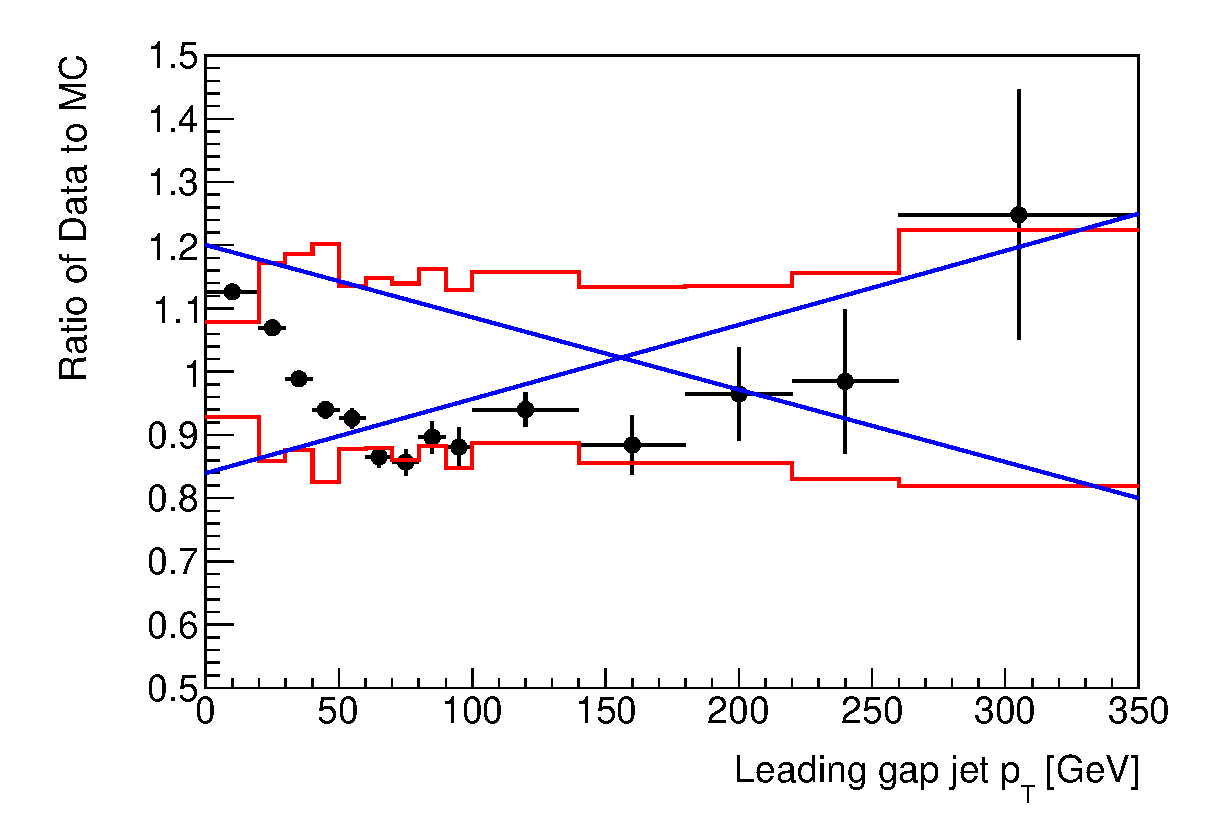
\includegraphics[width=0.8\textwidth]{figures/GBJ2/ControlPlots/Ratio___pt3.eps}
}
\caption[]{
Ratio of the \pt{} of the leading gap jet from 2010 uncorrected data to that of the reconstructed PYTHIA sample.
The red lines show the JES uncertainty bands.
\label{GBJ2:Uncorr:pt3}}
\end{figure}


\subsection{Combined Systematics}
\label{sec:GBJ2:SysComb}

The systematics studied above were combined  with a systematic from the unfolding process, which incorporates a MC statistics uncertainty and a model uncertainty, to produce the overall systematic uncertainty, some of which are shown in Figures \ref{GBJ2:SysComb:GapNjet} -- \ref{GBJ2:SysComb:cos2}.

Figure \ref{GBJ2:SysComb:GapNjet} shows the systematic uncertainty on (a) the gap fraction and (b) the average number of jets as a function of \dy{}
The dominant systematic is due to the JES uncertainty, while the unfolding also makes a significant contribution. 
The effect from JER is small, and the effect due to $\phi$ resolution is zero.


Figure \ref{GBJ2:SysComb:dphi23} shows the systematic uncertainty on the differential cross section for (a) inclusive events and (b) gap events.
The dominant systematics are again the JES uncertainty and the unfolding, while the effect from the $\phi$ resolution and the JER are small.

Figure \ref{GBJ2:SysComb:cos2} shows the systematic uncertainty on the average \costwodphi{} for (a) inclusive events and (b) gap events as a function of \dy{}.
For the inclusive distribution there is no overall dominant systematic, at low \dy{} $\phi$ resolution is large, with JES uncertainty, and unfolding also contributing.
While at large \dy{}, the uncertainty is dominated by the JES and unfolding.
For the gap distribution, again at low \dy{} the $\phi$ resolution is the dominant systematic and at larger \dy{} all the uncertainties have an effect. 

On the final plots, the combined systematic uncertainty is shown as a yellow band around the data point.


\begin{figure}
\centering
\mbox{
              \subfigure[]{\epsfig{figure=figures/GBJ2/FinalPlots/GapFraction_dyBins.systematics.eps,width=0.5\textwidth}}\quad
              \subfigure[]{\epsfig{figure=figures/GBJ2/FinalPlots/nGapJets_dyBins.systematics.eps,width=0.5\textwidth}}\quad
                              }
\caption[]{
The combined systematics on (a) the gap fraction and (b) the average number of jets in the dijet rapidity region as a function of \dy{}.
The combined systematics are from unfolding, JES uncertainty, JER and jet $\phi$ resolution.
\label{GBJ2:SysComb:GapNjet}}
\end{figure}
\begin{figure}
\centering
\mbox{
              \subfigure[]{\epsfig{figure=figures/GBJ2/FinalPlots/CrossSection.Inclusive.DPhiBins.2dY3.systematics.eps,width=0.5\textwidth}}\quad
              \subfigure[]{\epsfig{figure=figures/GBJ2/FinalPlots/CrossSection.Gap.DPhiBins.2dY3.systematics.eps,width=0.5\textwidth}}\quad
                              }
\caption[]{
The combined systematics on the differential cross section as a function of \dphi{}  for (a) inclusive events and (b) gap events for the \dy{} range 2--3.
The combined systematics are from unfolding, JES uncertainty, JER and jet $\phi$ resolution.
\label{GBJ2:SysComb:dphi23}}
\end{figure}


\begin{figure}
\centering
\mbox{
              \subfigure[]{\epsfig{figure=figures/GBJ2/FinalPlots/CosTwoDeltaPhiInclusive_dyBins.systematics.eps,width=0.5\textwidth}}\quad
              \subfigure[]{\epsfig{figure=figures/GBJ2/FinalPlots/CosTwoDeltaPhiGap_dyBins.systematics.eps,width=0.5\textwidth}}\quad
                              }
\caption[]{
The combined systematics on the average \costwodphi{} as a function of \dy{}  for (a) inclusive events and (b) gap events.
The combined systematics are from unfolding, JES uncertainty, JER and jet $\phi$ resolution.
\label{GBJ2:SysComb:cos2}}
\end{figure}


%\section{Assessment of Data vs MC Before Unfolding}
\label{sec:GBJ2:Uncorr}
This section presents the data compared to the reconstructed PYTHIA sample.
Figures \ref{GBJ2:Uncorr:Incl_Gap} -- \ref{GBJ2:Uncorr:Q0} show the uncorrected data compared to PYTHIA.
The PYTHIA error bands are the quadrature sum of the statistical error and the JES uncertainty bands. 

Figure \ref{GBJ2:Uncorr:Incl_Gap} shows (a) the gap fraction and (b) the mean number of jets in the region bounded by the dijet system, as a function of \dy{}.
The gap fraction measured from data falls as a function of \dy{}, up to $\dy{}>5.5$ where it starts to level off.
The PYTHIA gap fraction curve is consistently below the data up to a $\dy{}=6.5$.
PYTHIA then rises for the larges \dy{} bins, and has a higher gap fraction for $\dy{}>7$. 
The mean multiplicity of jets in the rapidity region increases as a function of \dy{}, to a peak of about $1.2$ at $\dy{}=7$, and then plateaus.
Both the flattening out of the gap fraction and the plateau in the mean number of jets could be due to PDF effects, such as those seen in the previous analysis for dijets with large \dy{} and \ptb{}.


Figures \ref{GBJ2:Uncorr:dphi23}, \ref{GBJ2:Uncorr:dphi45}, and \ref{GBJ2:Uncorr:dphi78} show \dphidyDist{} for $2<\dy{}<3$, $4<\dy{}<5$, and $7<\dy{}<8$,  respectively, for (a) inclusive events and (b) gap events.
PYTHIA does not describe the data particularly well, especially at high \dphi{} for  $2<\dy{}<3$ and $4<\dy{}<5$ slices where it is about $20\%$ below the data.
In the  $7<\dy{}<8$ slice, the PYTHIA results are still consistently below the data, but they agree within the JES uncertainty band.
The cross-section from PYTHIA does not agree with the measured cross-section, as there are large uncertainties in the leading order plus leading logarithm cross-section used by PYTHIA.

Figures \ref{GBJ2:Uncorr:cos} and \ref{GBJ2:Uncorr:cos2} show the \mean{\cosdphi{}} and \mean{\costwodphi{}} variables respectively, as a function of the dijet separation, \dy{}, for (a) inclusive and (b) gap events.
A \mean{\cosdphi{}} value of 1 corresponds to perfectly back-to-back jets in azimuth.
The \mean{\cosdphi{}} distribution for the inclusive events have a value of about $0.94$ for $\dy{}<2$.
As the $\dy{}$ increases, the jets become less back-to-back and the value of \mean{\cosdphi{}} falls and then levels off at a value of about $0.86$ for $\dy{}=6$.
As the $\dy{}$ increases, the available phase space to emit into is larger due to the jets being at very high energies.
For the gap events, the \mean{\cosdphi{}} at low \dy{} starts at a similar level to the inclusive events, but then slowly rises to a maximum of about $0.96$.
When the \dy{} is low, emissions can fall outside the rapidity region, but as the \dy{} increases this region becomes smaller, and the jet veto is stopping hard emission into the rapidity region, thus the dijets are more back-to-back.
The PYTHIA distribution show a slightly different shape from the data.
At both low and high \dy{}, the \mean{\cosdphi{}} for PYTHIA is higher than the data for both gap and inclusive events. 
In the range $2<\dy{}<5.5$, PYTHIA describes the data well.
The shape of the \mean{\costwodphi{}} distribution has a similar explanation to the \mean{\cosdphi{}} distribution, and shows similar features.
For both inclusive and gap events, PYTHIA's description of \mean{\costwodphi{}} is too low at low \dy{} and too high at high \dy{}.

Figure \ref{GBJ2:Uncorr:Q0} shows the gap fraction as a function of the jet veto scale, \qz{}, for the \dy{} ranges $2<\dy{}<3$, $4<\dy{}<5$, and $7<\dy{}<8$.
As \qz{} is increased, fewer events are defined as gap events, until at high \qz{} the gap fraction is at $1.0$.
In the range $2<\dy{}<3$, the PYTHIA gap fraction is lower than the data for $\qz{}<50$ GeV, though it is within the JES uncertainty.
In the range $4<\dy{}<5$, the PYTHIA gap fraction describes the data well for the full \qz{} range.
For dijets within the range $7<\dy{}<8$, the PYTHIA gap fraction is higher than the data until both gap fractions plateau at $1.0$.

\begin{figure}
\centering
        \begin{subfigure}[b]{0.5\textwidth}
                \centering
                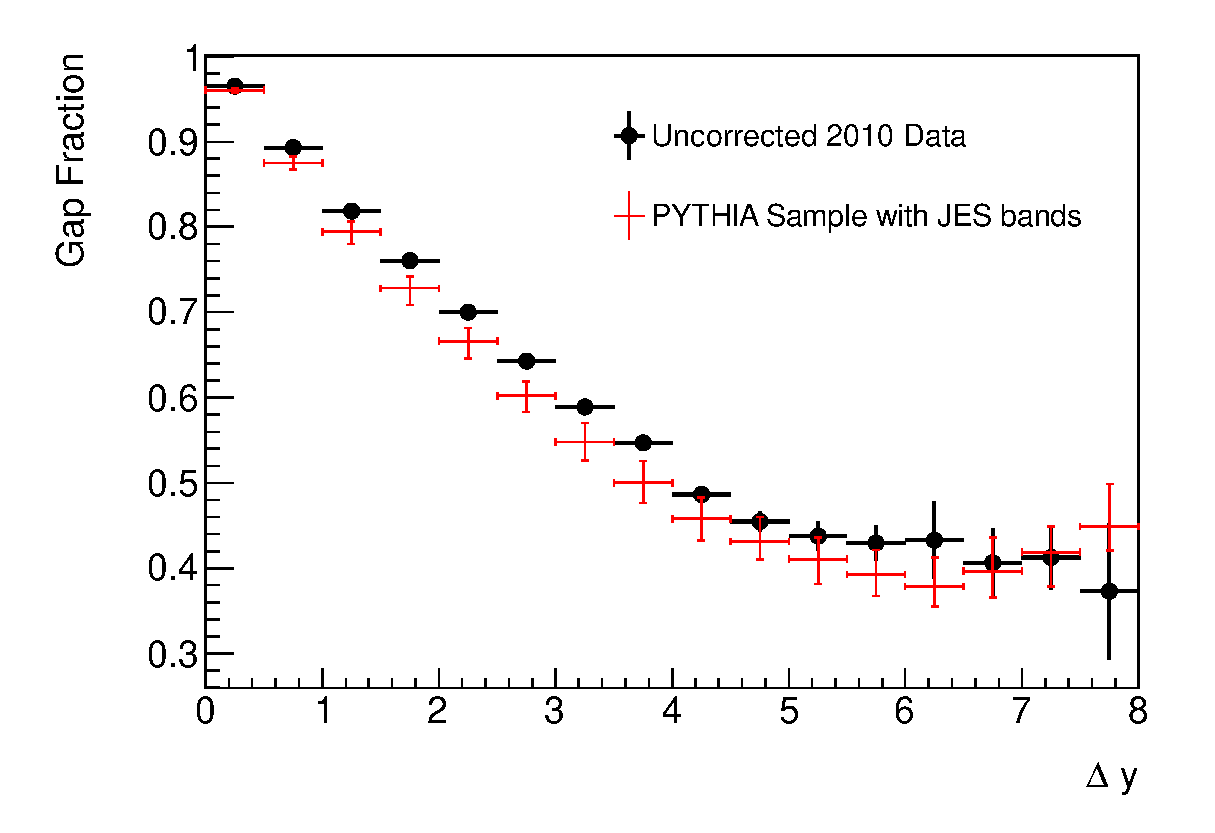
\includegraphics[width=\textwidth]{figures/GBJ2/ControlPlots/Smeared__GapFraction_deltaY.eps}
        \end{subfigure}%
        \begin{subfigure}[b]{0.5\textwidth}
                \centering
                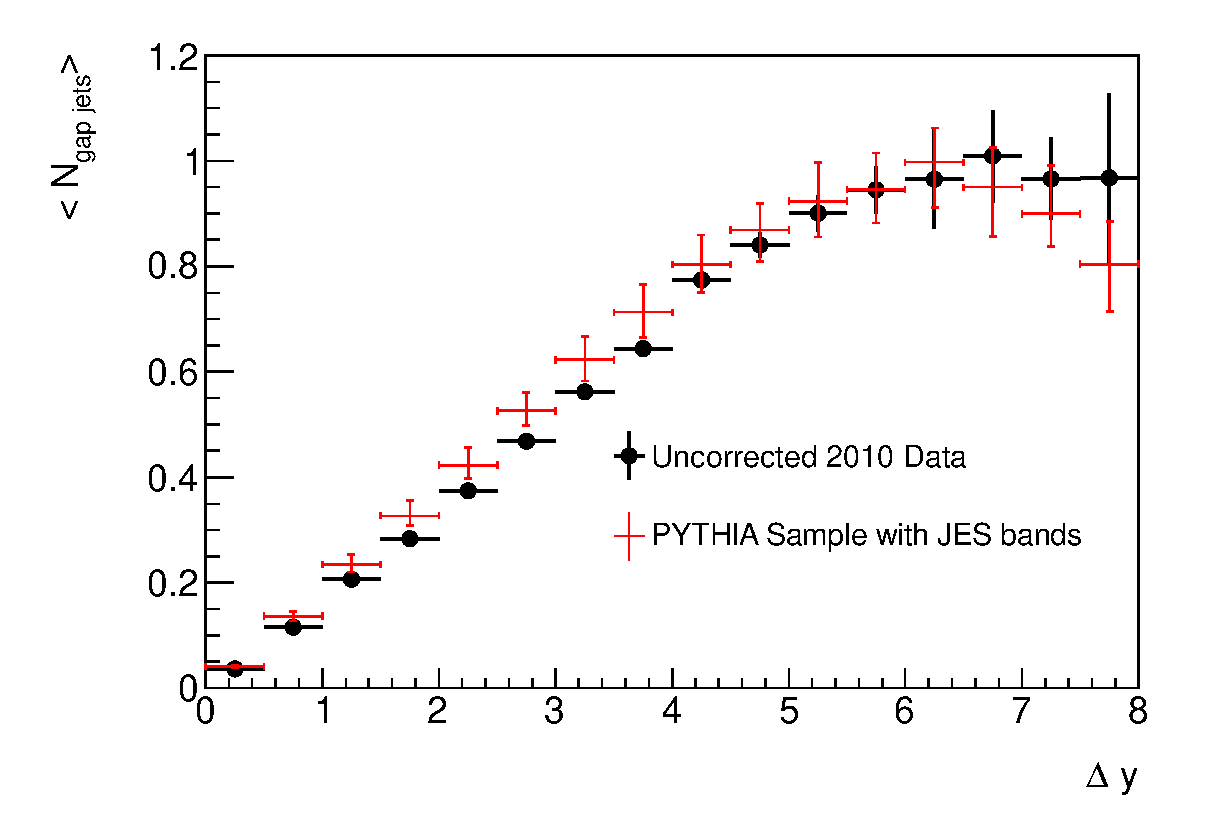
\includegraphics[width=\textwidth]{figures/GBJ2/ControlPlots/Smeared__prof_deltaY_njets.eps}
        \end{subfigure}%
\caption[Comparison of the data and PYTHIA for the gap fraction and mean number of jets]{
(a) The gap fraction  and (b) the mean number of jets in the rapidity region bounded by the dijet system as a function of \dy{} for 2010 uncorrected data (black points) and reconstructed PYTHIA sample (red points).
\label{GBJ2:Uncorr:Incl_Gap}}
\end{figure}



\begin{figure}
\centering
        \begin{subfigure}[b]{0.5\textwidth}
                \centering
                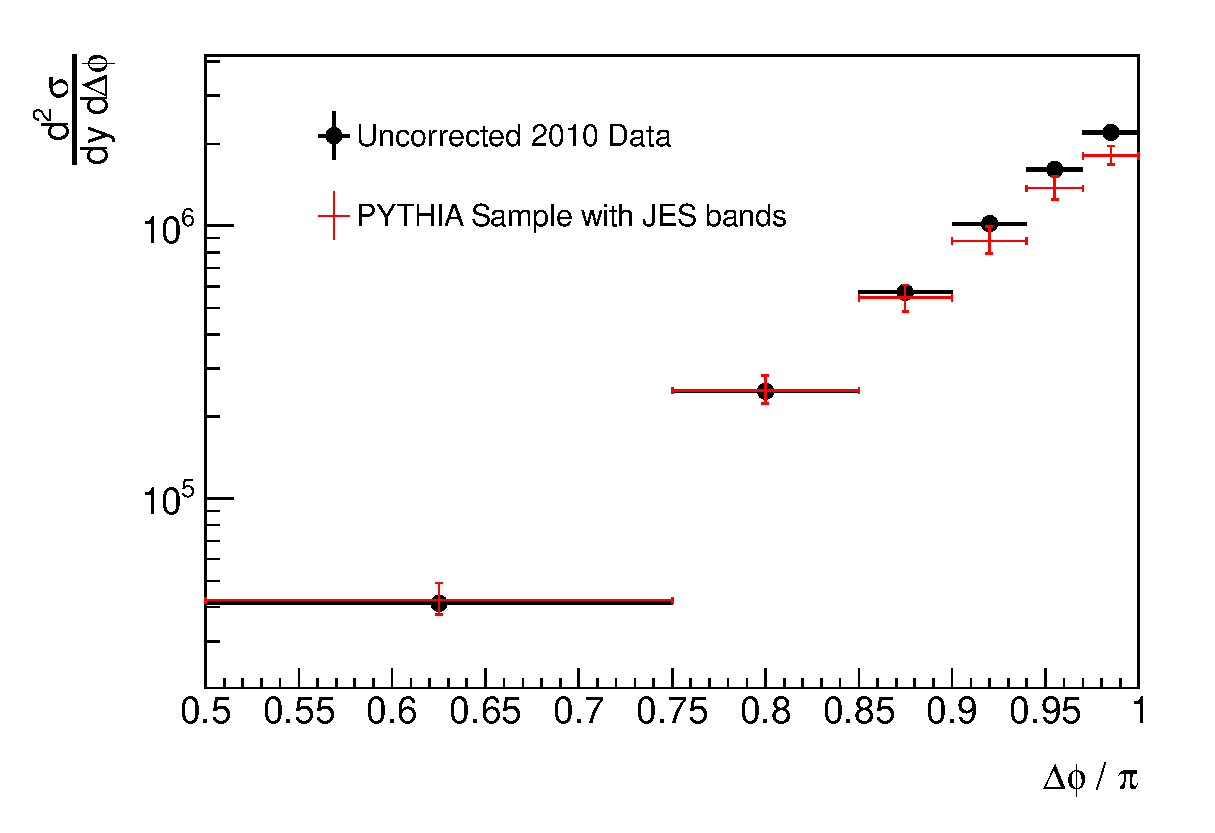
\includegraphics[width=\textwidth]{figures/GBJ2/ControlPlots/Smeared__dPhi__2_3.eps}
        \end{subfigure}%
        \begin{subfigure}[b]{0.5\textwidth}
                \centering
                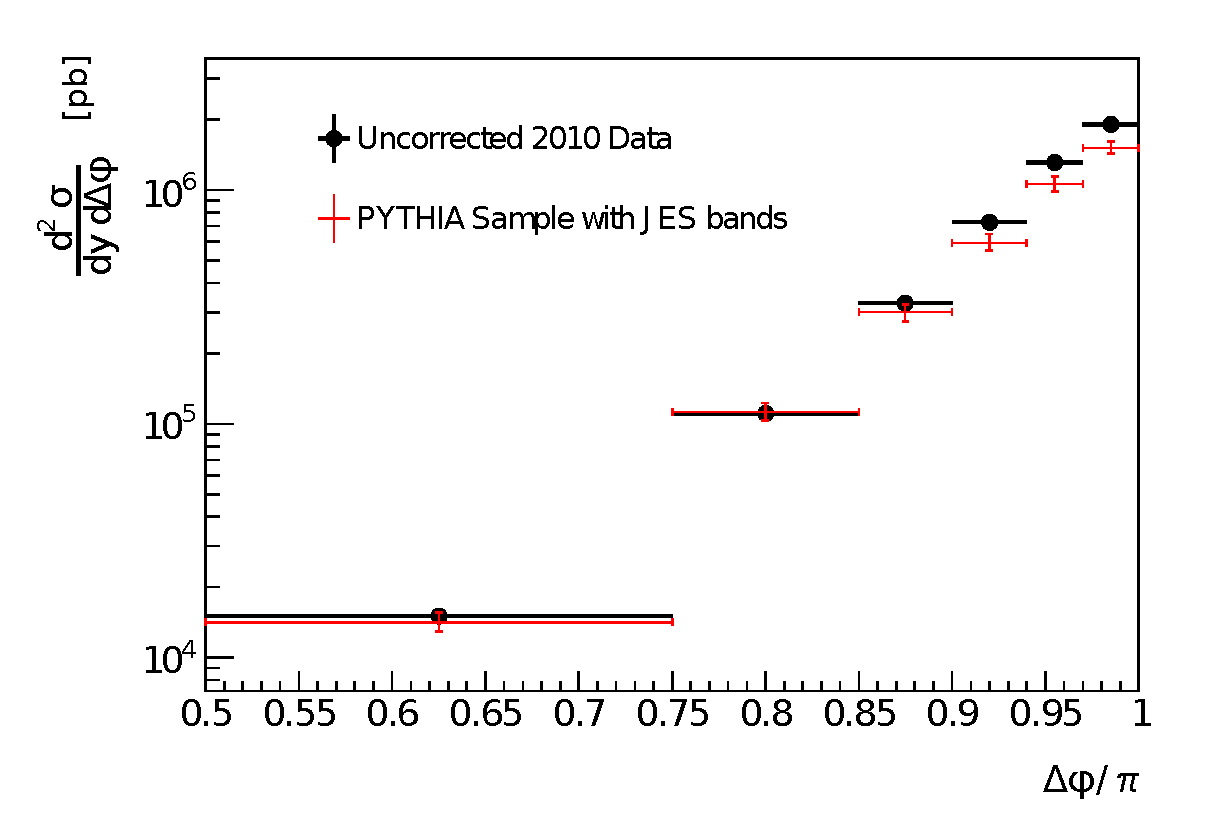
\includegraphics[width=\textwidth]{figures/GBJ2/ControlPlots/Smeared__dPhi_gap__2_3.eps}
        \end{subfigure}%
\caption[Comparison of the data and PYTHIA for \dphidyDist{} with $2<\dy{}<3$]{
\dphidyDist{} for (a) inclusive events and (b) gap events for a dijet separation, \dy{} of 2-3 for 2010 uncorrected data (black points) and reconstructed PYTHIA sample (red points).
\label{GBJ2:Uncorr:dphi23}}
\end{figure}


\begin{figure}
\centering
        \begin{subfigure}[b]{0.5\textwidth}
                \centering
                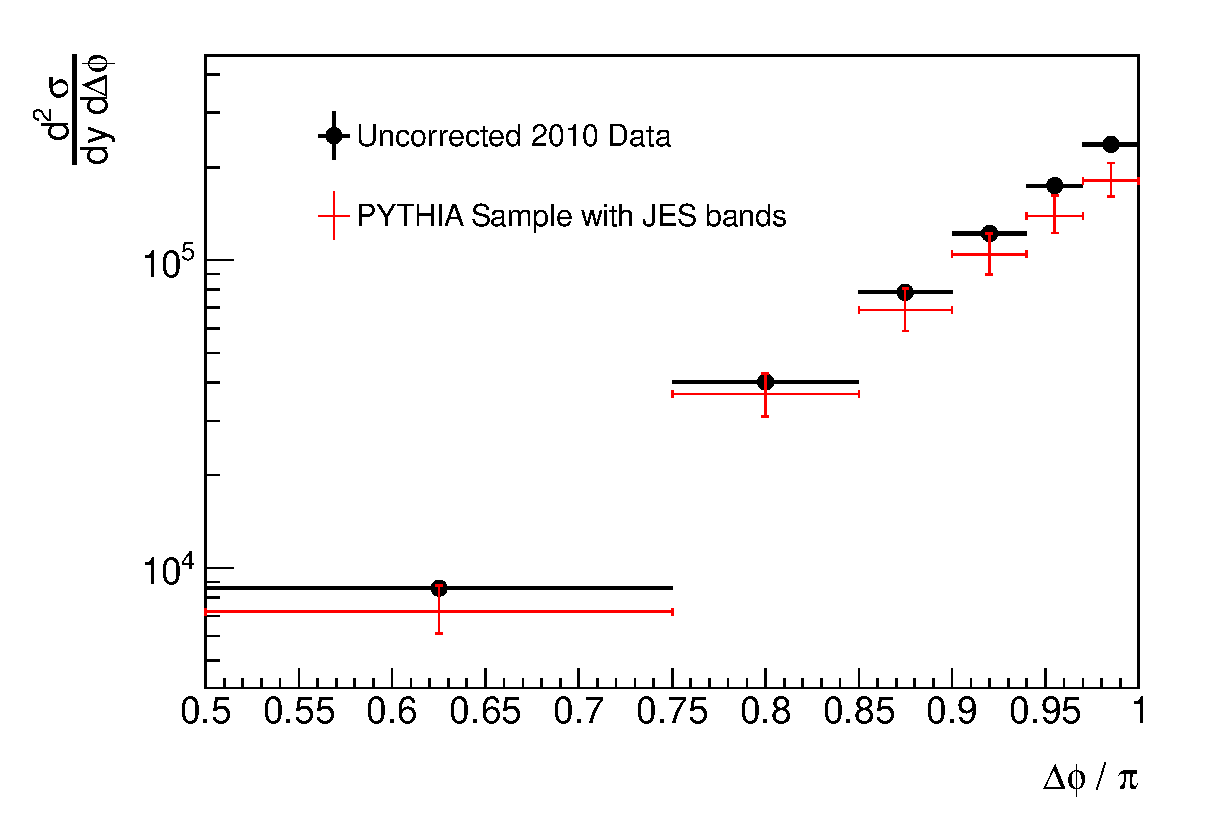
\includegraphics[width=\textwidth]{figures/GBJ2/ControlPlots/Smeared__dPhi__4_5.eps}
        \end{subfigure}%
        \begin{subfigure}[b]{0.5\textwidth}
                \centering
                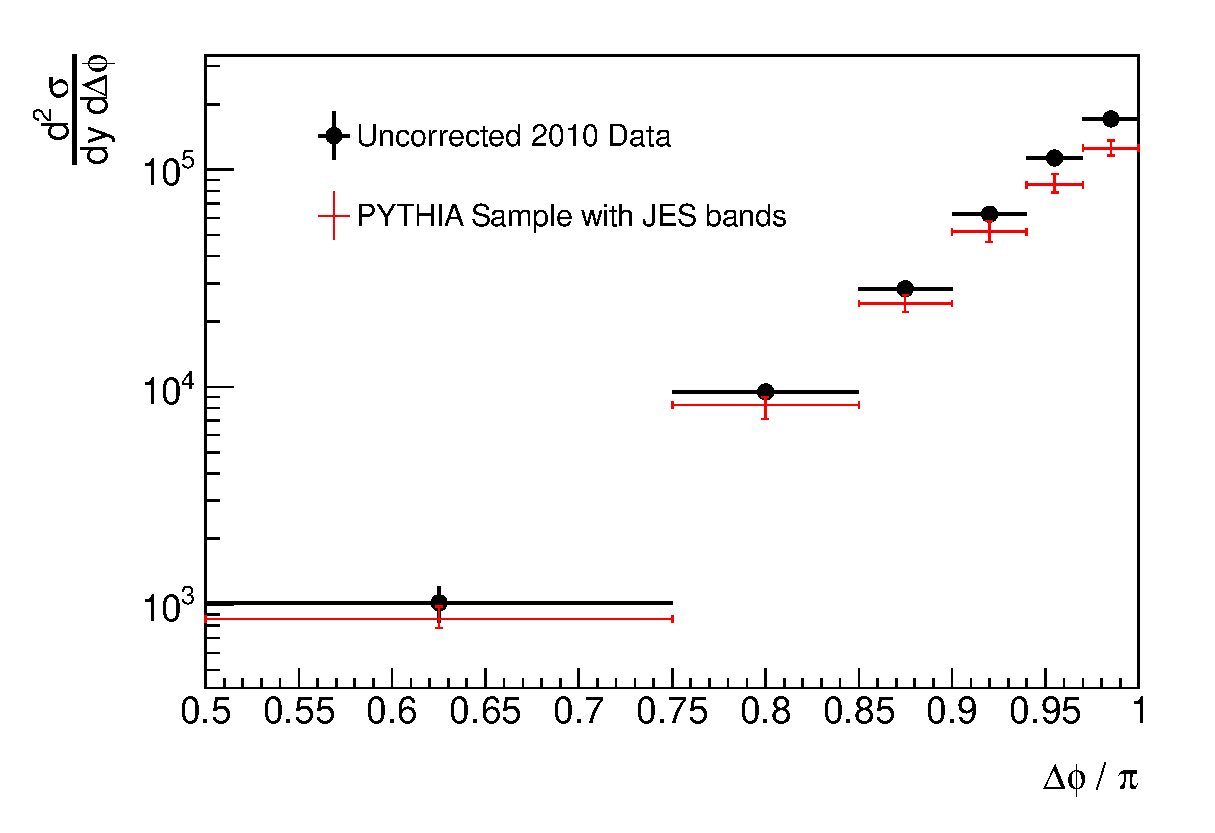
\includegraphics[width=\textwidth]{figures/GBJ2/ControlPlots/Smeared__dPhi_gap__4_5.eps}
        \end{subfigure}%
\caption[Comparison of the data and PYTHIA for \dphidyDist{} with $4<\dy{}<5$]{
\dphidyDist{} for (a) inclusive events and (b) gap events for a dijet separation, \dy{} of 4-5 for 2010 uncorrected data (black points) and reconstructed PYTHIA sample (red points).
\label{GBJ2:Uncorr:dphi45}}
\end{figure}



\begin{figure}
\centering
        \begin{subfigure}[b]{0.5\textwidth}
                \centering
                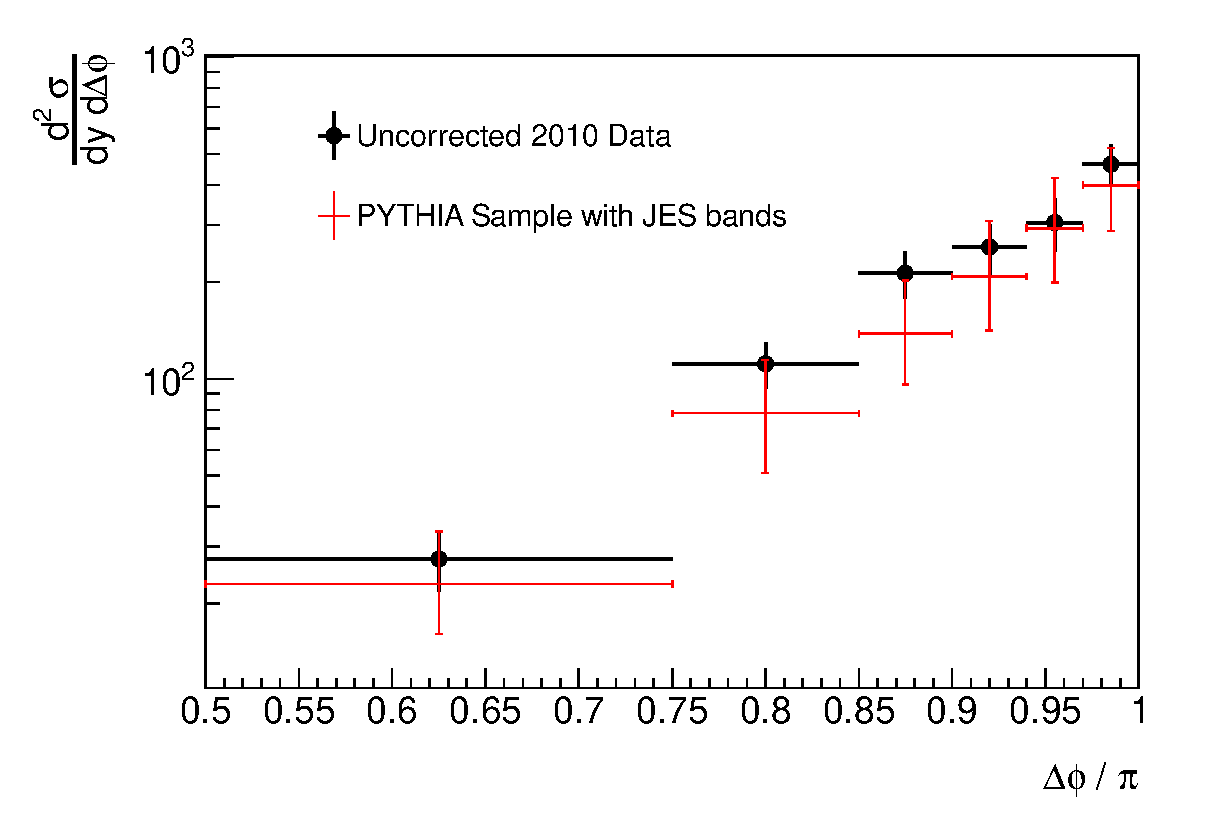
\includegraphics[width=\textwidth]{figures/GBJ2/ControlPlots/Smeared__dPhi__7_8.eps}
        \end{subfigure}%
        \begin{subfigure}[b]{0.5\textwidth}
                \centering
                \includegraphics[width=\textwidth]{figures/GBJ2/ControlPlots/Smeared__dPhi_gap__7_8.eps}
        \end{subfigure}%
\caption[Comparison of the data and PYTHIA for \dphidyDist{} with $7<\dy{}<8$]{
\dphidyDist{} for (a) inclusive events and (b) gap events for a dijet separation, \dy{} of 7-8 for 2010 uncorrected data (black points) and reconstructed PYTHIA sample (red points).
\label{GBJ2:Uncorr:dphi78}}
\end{figure}



\begin{figure}
\centering
        \begin{subfigure}[b]{0.5\textwidth}
                \centering
                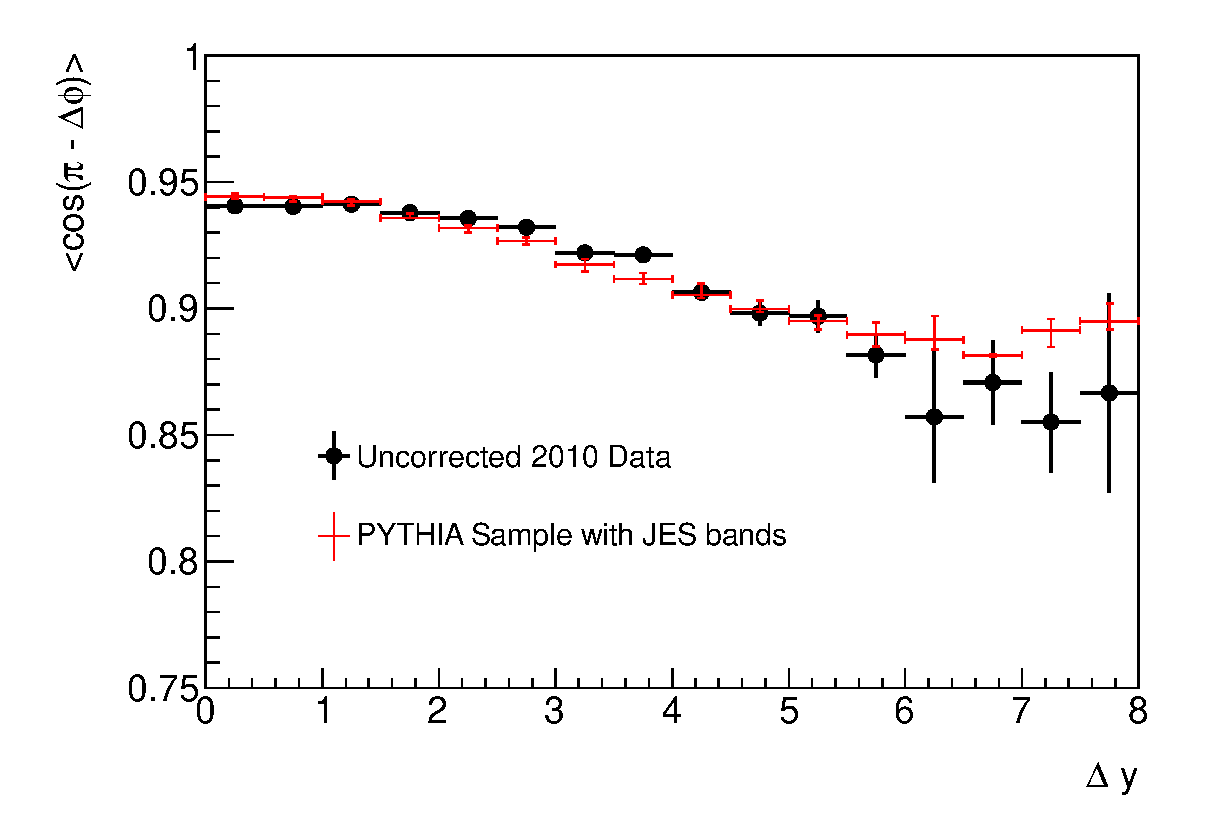
\includegraphics[width=\textwidth]{figures/GBJ2/ControlPlots/Smeared__cosdPhi_deltaY.eps}
        \end{subfigure}%
        \begin{subfigure}[b]{0.5\textwidth}
                \centering
                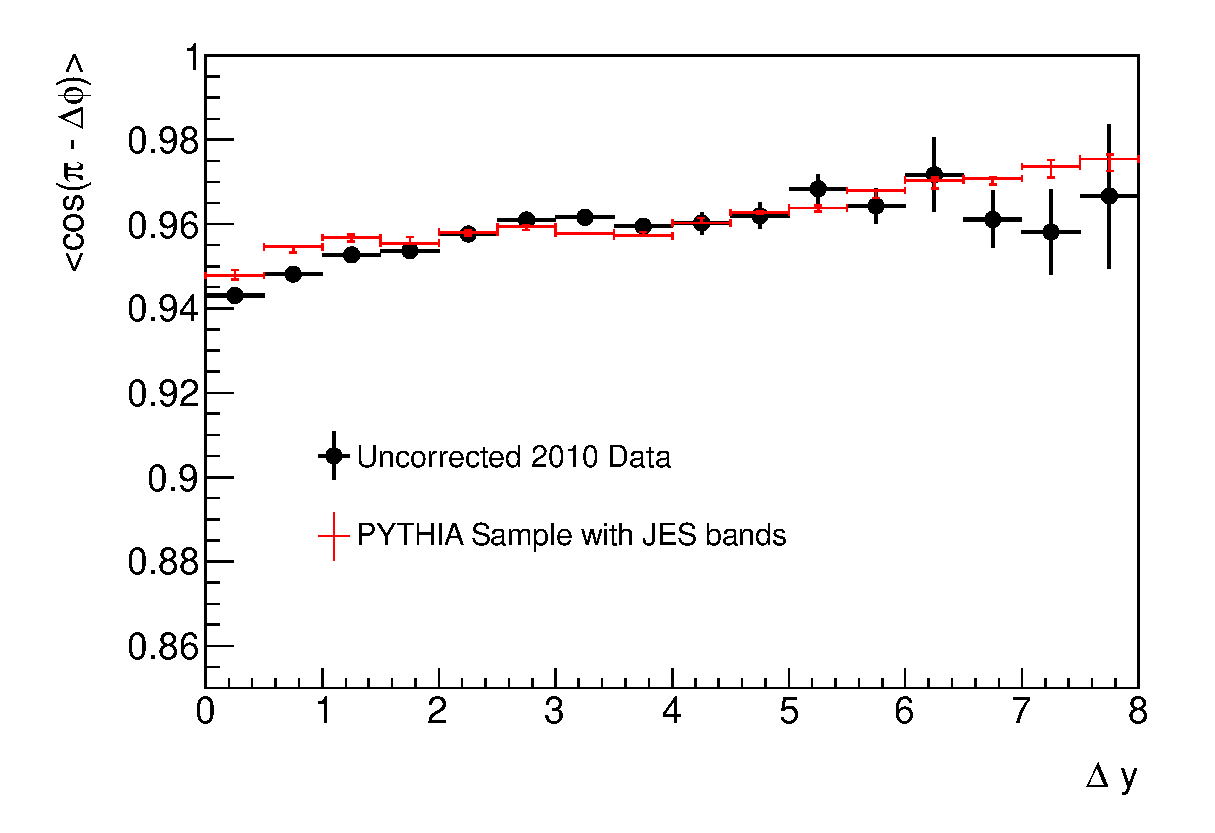
\includegraphics[width=\textwidth]{figures/GBJ2/ControlPlots/Smeared__cosdPhi_deltaY_gap.eps}
        \end{subfigure}%
\caption[Comparison of the data and PYTHIA for \cosdphi{}]{
\mean{\cosdphi{}} as a function of \dy{} for (a) inclusive and (b) gap events for 2010 uncorrected data (black points) and reconstructed PYTHIA sample (red points).
\label{GBJ2:Uncorr:cos}}
\end{figure}


\begin{figure}
\centering
        \begin{subfigure}[b]{0.5\textwidth}
                \centering
                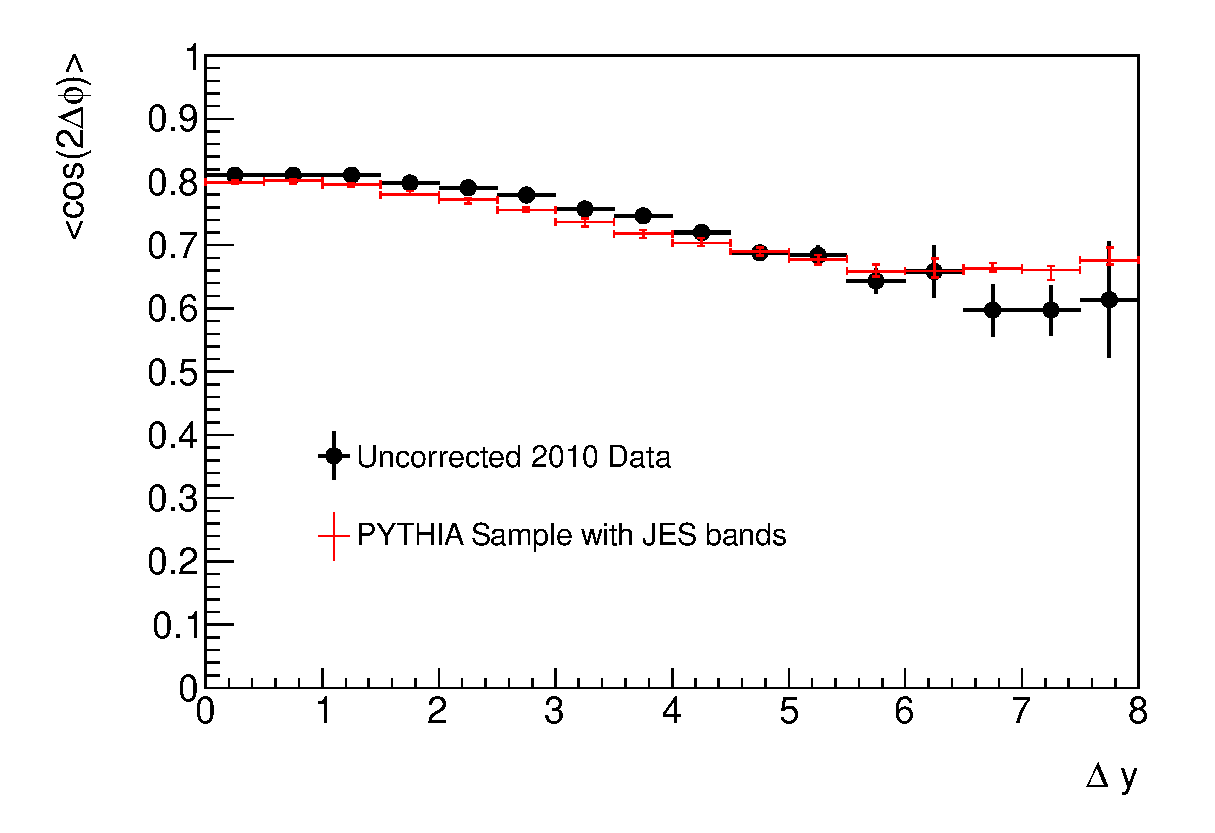
\includegraphics[width=\textwidth]{figures/GBJ2/ControlPlots/Smeared__cos2dPhi_deltaY.eps}
        \end{subfigure}%
        \begin{subfigure}[b]{0.5\textwidth}
                \centering
                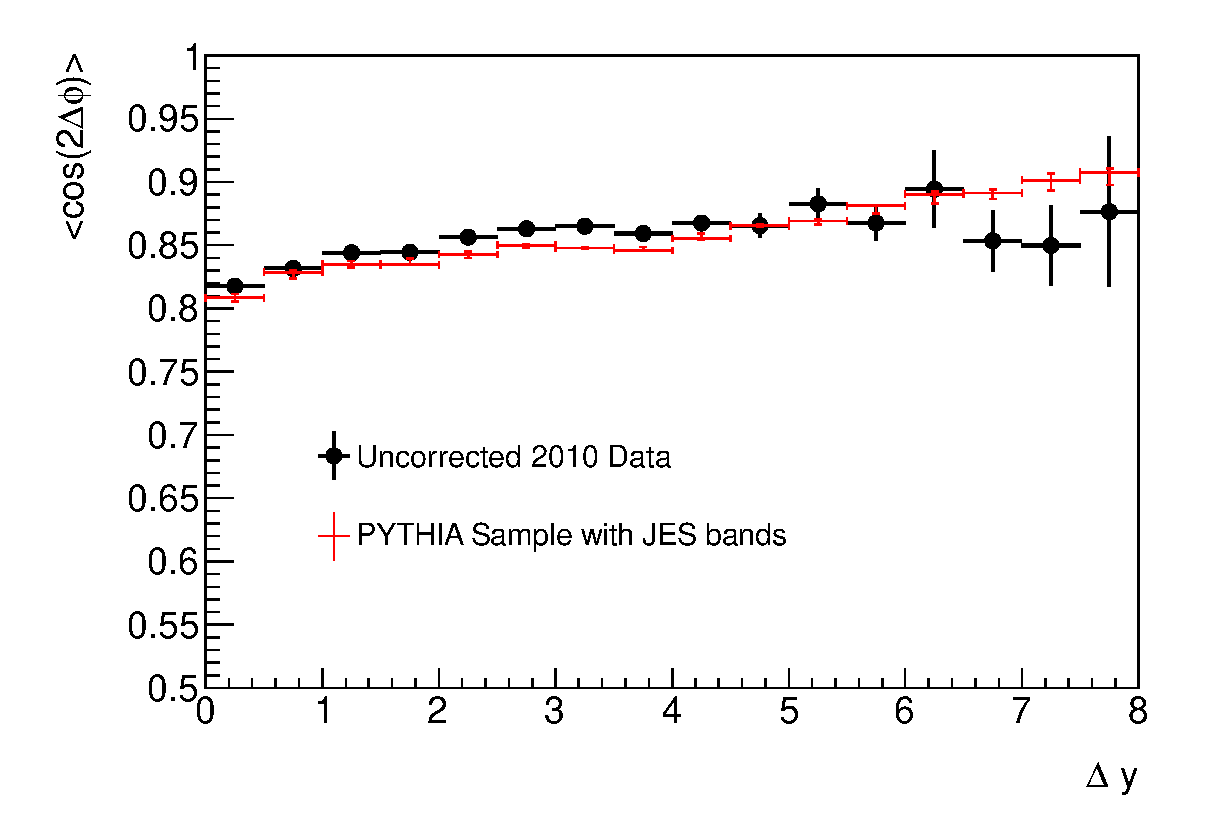
\includegraphics[width=\textwidth]{figures/GBJ2/ControlPlots/Smeared__cos2dPhi_deltaY_gap.eps}
        \end{subfigure}%
\caption[Comparison of the data and PYTHIA for \costwodphi{}]{
\mean{\costwodphi{}} as a function of \dy{} for (a) inclusive and (b) gap events for 2010 uncorrected data (black points) and reconstructed PYTHIA sample (red points).
\label{GBJ2:Uncorr:cos2}}
\end{figure}

\begin{figure}
\centering
        \begin{subfigure}[b]{0.5\textwidth}
                \centering
                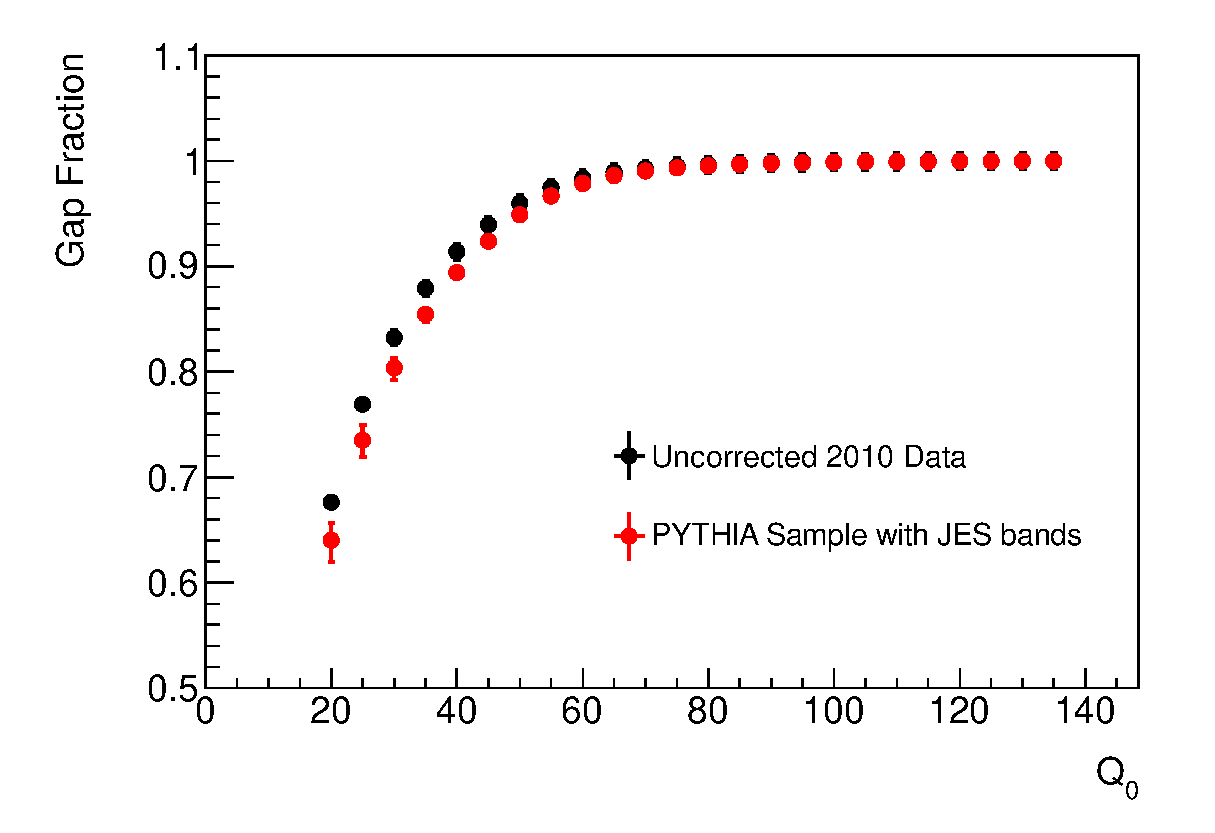
\includegraphics[width=\textwidth]{figures/GBJ2/ControlPlots/Smeared2_3__Q0.eps}
        \end{subfigure}%
        \begin{subfigure}[b]{0.5\textwidth}
                \centering
                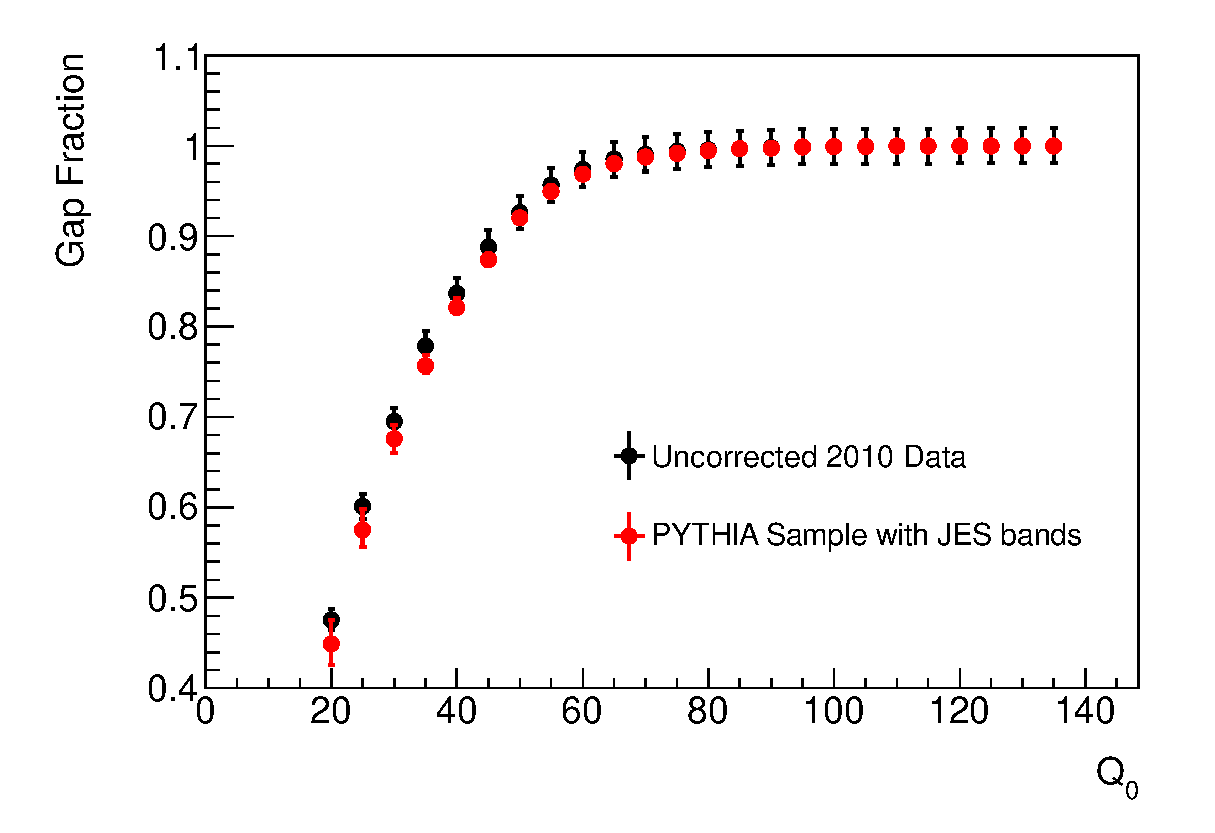
\includegraphics[width=\textwidth]{figures/GBJ2/ControlPlots/Smeared4_5__Q0.eps}
        \end{subfigure}%


        \begin{subfigure}[b]{0.5\textwidth}
                \centering
                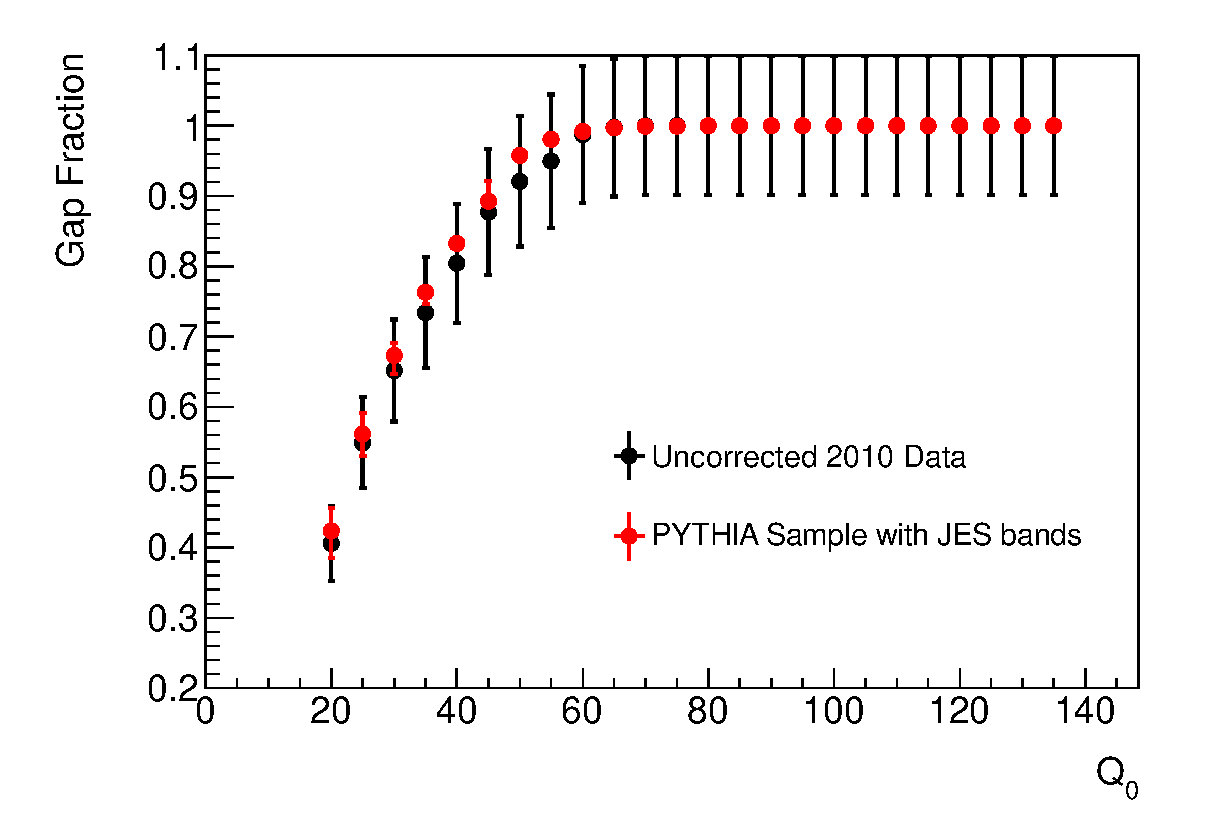
\includegraphics[width=\textwidth]{figures/GBJ2/ControlPlots/Smeared7_8__Q0.eps}
        \end{subfigure}%
\caption[Comparison of the data and PYTHIA for the gap fraction as a function of \qz{}]{
The gap fraction against \qz{} for (a) $2<\dy{}<3$, (b) $4<\dy{}<5$ and (c) $7<\dy{}<8$ for 2010 uncorrected data (black points) and reconstructed PYTHIA sample (red points).
\label{GBJ2:Uncorr:Q0}}
\end{figure}


%This analysis is currently in internal review within ATLAS and being combined with other associated analyses.


\chapter{Summary and Conclusions}
\label{chp:Conc}
\input{Conclusion/conclusions.tex}

\bibliographystyle{mnras}
%\bibliographystyle{atlasnote}
\bibliography{references}
\end{document}
